\documentclass[a4paper,oneside,12pt]{book}

\newcommand{\thesistitle}{Predicting the features of Steam reviews and determining representative users with BERT}
\newcommand{\degree}{Master in Computer Science}
\newcommand{\typeofthesis}{dissertation}
\newcommand{\authorname}{Conor McCauley}
\newcommand{\keywords}{example}
\newcommand{\school}{\href{http://www.scss.tcd.ie}{School of Computer Science and Statistics}}

\AtBeginDocument{
    \hypersetup{pdftitle=\thesistitle}
    \hypersetup{pdfauthor=\authorname}
    \hypersetup{pdfkeywords=\keywords}
    \hypersetup{pdfsubject=\degree}
}

\usepackage[hyphens]{url}
\usepackage[T1]{fontenc} 
\usepackage[utf8]{inputenc}
\usepackage[english]{babel}
\usepackage[round,sort,comma,numbers]{natbib}
\usepackage[a4paper,top=2.54cm,bottom=2.54cm,left=2.54cm,right=2.54cm,headheight=16pt]{geometry}
\setlength{\marginparwidth}{2cm}
\usepackage{amsmath}
\usepackage[autostyle=true]{csquotes}
\usepackage[pdftex]{graphicx}
\usepackage[colorinlistoftodos]{todonotes}
\usepackage[colorlinks=true, allcolors=black]{hyperref}
\usepackage{caption}
\usepackage{subcaption}
\usepackage[parfill]{parskip}
\usepackage{setspace}
\usepackage{enumerate}
\usepackage{booktabs}
\usepackage{fancyhdr}
\usepackage{listings}
\usepackage{xcolor}
\usepackage{multirow}
\usepackage[symbol]{footmisc}
\usepackage[section]{placeins}
\pagestyle{plain}

\renewcommand{\familydefault}{\sfdefault}
%\usepackage{mathpazo}

\renewcommand{\theequation}{\arabic{equation}}
\renewcommand{\lstlistlistingname}{List of \lstlistingname s}

\usepackage{titlesec}
\titleformat{\chapter}[hang] 
{\normalfont\huge\bfseries}{\thechapter}{1cm}{} 
\setcounter{secnumdepth}{4}
\titleformat{\paragraph}{\normalfont\normalsize\bfseries}{\theparagraph}{1em}{}
\titlespacing*{\paragraph}{0pt}{3.25ex plus 1ex minus .2ex}{1.5ex plus .2ex}

\title{\thesistitle}
\author{\authorname}

\frontmatter
\begin{document}
\begin{titlepage}

\center

\includegraphics{title/logo_col.png}\\[1cm] 
\Large \school\\[1.5cm]
\ifdefined\department
\large \department\\[1.5cm]
\fi

\makeatletter
{ \huge \bfseries \thesistitle}\\[1.5cm]
    
\ifdefined\authorid
\authorname\\
\authorid\\[2cm]
\else
\authorname\\[2cm]
\fi

{\large \today}\\[2cm]
    
\vfill
    A \typeofthesis\ submitted in partial fulfilment\\of the requirements for the degree of\\
\degree

\vfill

\end{titlepage}

\pagenumbering{roman}
\section*{\Huge{Declaration}}
\vspace{1cm}
I hereby declare that this \typeofthesis\ is entirely my own work and that it has not been submitted as an exercise for a degree at this or any other university.

\vspace{1cm}
I have read and I understand the plagiarism provisions in the General Regulations of the University Calendar for the current year, found at \url{http://www.tcd.ie/calendar}.
\vspace{1cm}

I have also completed the Online Tutorial on avoiding plagiarism `Ready Steady Write', located at \url{http://tcd-ie.libguides.com/plagiarism/ready-steady-write}.
\vspace{3cm}

Signed:~\rule{5cm}{0.3pt}\hfill Date:~\rule{5cm}{0.3pt}

\chapter*{Abstract}

The video game industry is hugely popular and rapidly growing, generating over 179 billion US dollars in global revenue in 2020, an increase of 20\% over the previous year. The Steam platform, a video game distribution service that is the largest of its kind, is used by over 120 million users every month and provides a selection of over 60 thousand games.

This dissertation used a dataset of over 10 million video game reviews, taken from Steam, to investigate the degree to which the text of a review can be used by machine learning models, such as BERT, to predict other features of the review. The particular review features that were investigated were the review polarity, the community-determined helpfulness of the review and the amount of time the reviewer spent playing the game before reviewing it.

This investigation was also expanded upon and used to develop a method to determine which reviewers are most representative of the overall population using a somewhat novel approach. The methodology underpinning this new approach, the assumptions made when implementing it and the drawbacks that it presented were discussed. Potential improvements and refinements, alongside potential commercial applications, were also suggested.

The results of the review feature prediction were mixed. The polarity of reviews was able to be accurately predicted, with accuracies reaching as high as 85.9\% for balanced data samples and 91.3\% for imbalanced samples. The models developed to predict review helpfulness did not prove successful, while the models developed to predict reviewer playtimes produced uncertain results. The models developed to determine representative users performed sufficiently better than baseline models, indicating that the approach, even in its simplest form, bears potential for further investigation. The model was then used to successfully identify users that it considered to be representative.

\newpage
\onehalfspacing\raggedright

\section*{\Huge{Acknowledgements}}

I would like to express my gratitude towards Professor Douglas Leith for originally formulating the topic of this dissertation and for continually providing me with valuable advice and suggestions over the past few months.

I would also like to thank my parents for all of the help and support they've given me throughout my studies.

\tableofcontents
\listoffigures
\listoftables
\lstlistoflistings
\newpage

\section*{\Huge{Nomenclature}}
\begin{tabular}{lp{9cm}l}
AUC&Area Under the Curve\\
BERT&Bidirectional Encoder Representations from Transformers\\
CNB&Complement Naive Bayes\\
CNN&Convolutional Neural Network\\
FPR&False Positive Rate\\
LSVC&Linear Support Vector Classifier\\
LSVR&Linear Support Vector Regressor\\
MNB&Multinomial Naive Bayes\\
MSE&Mean Squared Error\\
NB&Naive Bayes\\
NLP&Natural Language Processing\\
NMSE&Negative Mean Squared Error\\
RNN&Recurrent Neural Network\\
ROC&Receiver Operating Characteristic\\
SD&Standard Deviation\\
SGD&Stochastic Gradient Descent\\
SVM&Support Vector Machine\\
TF-IDF&Term Frequency-Inverse Document Frequency\\
TPR&True Positive Rate\\
\end{tabular}
\vspace{2cm}

\mainmatter

\chapter{Introduction} \label{sec:Intro}

\section{Overview and Motivation} \label{sec:Intro_Overview}

The video game industry is hugely popular and rapidly growing. In 2020, the industry generated over 179 billion US dollars in global revenue, an increase of 20\% over the previous year \cite{GamingIndustrySize}. The Steam platform, a video game distribution service, is the largest of its kind for PC users \cite{SteamLargestDistributor} with over 120 million active monthly users \cite{SteamMonthlyUsers} and a selection of over 60 thousand games \cite{SteamGameCount}.

This dissertation will make use of a large collection of data taken from the Steam platform via its public API. This dataset primarily consists of extensive information regarding the game reviews that users have written; however, it also contains social information about the reviewers, such as who they are friends with and the gaming communities that they are involved in.

The primary motivations behind this project are twofold. The first involves determining whether the written text of Steam reviews can be used by machine learning models to predict other features of the review, and, if so, to what extent are these predictions accurate or reliable. The review features being predicted might include the review's polarity/sentiment; its helpfulness, as determined by other users; or the amount of time the reviewer had spent playing the game prior to writing their review. The second motivation involves the development of a method to identify particularly representative users among the entire population using only the written text of the reviews. A representative user is considered to be someone whose ratings or opinions of games tend to align with the population as a whole, thus acting as a reliable and valuable source of information as to how a new game, or any product, for that matter, might be received by other users.

The dataset will be comprehensively examined prior to designing and implementing the above approaches. This examination will make use of plots and visualisations in order to provide a deeper understanding of the nature of the reviews, the users and the Steam platform itself. Some of the dataset characteristics that will be examined are the number of reviews that users write, the languages in which reviews are written, the lengths of the reviews, the proportion of reviews that are positive or negative, the number of reviews that are considered helpful by other users, and the lengths of time that reviewers spend playing the games they review. This examination will provide crucial insight into the underlying structure of both Steam and the dataset which will help inform and guide the design and implementation of the aforementioned approaches.

The first research motivation will utilise state-of-the-art language representation techniques, such as BERT, to investigate the predictive validity of models trained using only the review text. Detailed analysis will be performed to determine the effect that specific text features have on the models' results. These text features might include the word count, the language the review was written in or how balanced the distribution of the output feature being predicted is. The results of the experiments, both positive and negative, will be discussed and a number of potential improvements will be suggested.

The second research motivation will involve building upon the results of the first, ie whether or not the review text is informative and can be used to make reliable predictions about other features. The employed approach will involve the development of a machine learning classifier that will use review texts to predict the overall rating of the game being reviewed. The resulting model, assuming it is found to be sufficiently accurate, will be evaluated for each individual reviewer in order to determine those users whose combinations of review text and game ratings the model is most capable of predicting accurately. Different methods of selecting the most representative users will be examined and compared. The methodology behind this approach, which seems to be somewhat novel, will be explained and justified; the assumptions made during its design, as well as the numerous drawbacks that it presents, will also be discussed. A myriad of potential ways to improve upon or refine the approach will be suggested. Finally, a selection of real world, commercial applications of this research, mainly related to recommender systems, will be proposed.

This research appears to be well suited to platforms such as Steam due to the gaming industry's rapid increase in popularity and tremendous economic value. As a result of the abundance of new games being released, a method of quickly and reliably determining whether or not a new game is worth recommending to users would be of considerable value to platforms like Steam as a means of increasing total sales as well as user retention and satisfaction. This determination could be done using methods based on those that will be outlined in this report.

\section{Dissertation Structure} \label{sec:Intro_Structure}

This dissertation will consist of eight chapters, including this one. In chapter \ref{sec:LR}, an overview of the existing literature will be provided. In chapter \ref{sec:BG}, the structure and functionality of both the Steam platform and the dataset will be described in greater detail. Chapter \ref{sec:Dataset} will consist of an in depth examination of the dataset, accompanied by numerous visualisations. In chapter \ref{sec:TBG}, technical descriptions and explanations will be provided for each of the machine learning methods, techniques and evaluation metrics utilised throughout the dissertation. Chapter \ref{sec:DI} will provide a thorough description of the approaches used to achieve the research objectives, while chapter \ref{sec:Res} will present and discuss the results of these approaches. In chapter \ref{sec:Conc}, the dissertation will be concluded, with the overall results of the research being summarised and assessed.

\chapter{Literature Review}  \label{sec:LR}

\section{Natural Language Processing} \label{sec:LR_NLP}

In computer science and, in particular, artificial intelligence, the field of natural language processing (NLP) concerns the representation, analysis and utilisation of human language, in both written and spoken form, by computers. NLP traces its origins to the 1950s when an IBM computer was used to translate a number of Russian sentences into English at Georgetown University \cite{Hutchins2004_MT}.

Modern applications of NLP are ubiquitous, ranging from spam detection \cite{Jindal2007_Spam} to chatbots \cite{Adamopoulou2020_Chatbot}. Specific examples of its use include machine translation tools, such as Google Translate \cite{GoogleTranslate}, that can translate text from one language to another; speech recognition software, such as Microsoft's Cortana \cite{MicrosoftSpeechRecognition}, which can recognise spoken words from audio of human speech; sentiment analysis techniques to determine the sentiment or the emotions conveyed through text which have been used to determine public opinion on topics such as political preferences \cite{Ceron2014_Sentiment}; and question answering systems, such as IBM's Watson, that can respond to questions asked by humans and have been used to make decisions regarding the treatment of cancer patients \cite{AOCNP2015_Watson}.

The state-of-the-art in human language encoding and representation involves the use of transformers, a type of neural network developed by Google \cite{Vaswani2017_Transformers}, which differ from recurrent neural networks (RNN), the prior state-of-the-art, in that they attempt to simulate the process of attention in humans by increasing the weight of certain segments of input data and decreasing the weight of others \cite{Bahdanau2014_Attention}.

Bidirectional Encoder Representations from Transformers (BERT) is an NLP model developed by Google which, when published in 2018, achieved state-of-the-art results in numerous popular NLP tasks such as GLUE and SQuAD v1.1 and v2.0 \cite{Devlin2018_BERT}. BERT, unlike some other language representation models, such as word2vec \cite{Mikolov2013_W2V}, considers the context of each token in any given text data, ie the tokens that come before and after it. An advantage of BERT is, according to \cite{Devlin2018_BERT}, that it ``can be fine-tuned with just one additional output layer \ldots without substantial task-specific architecture modifications''. BERT is used to process almost all English-language Google Search queries \cite{GoogleSearchBERT}.

\subsection{Product Review Sentiment} \label{sec:LR_NLP_Sent}

Substantial research has been done in the field of NLP with regards to text classification and, in particular, sentiment analysis \cite{mironczuk2018recent}. Much of this research has concerned the classification of user sentiment in product reviews.

Support vector machine (SVM) and naive Bayes (NB) classifiers were use to predict the polarities of Amazon book reviews, represented using the term frequency-inverse document frequency (TF-IDF) model, in \cite{dey2020comparative}. The SVM classifier, which had an accuracy score of 84\%, slightly outperformed the NB classifier, which had an accuracy score of 82.8\%. In \cite{aljuhani2019comparison}, the polarities of a balanced set of Amazon phone reviews were predicted using, among others, NB, stochastic gradient descent (SGD) and convolutional neural network (CNN) classifiers. TF-IDF and neural network techniques, such as word2vec, were used to represent the review text. The combination of the CNN classifier and word2vec produced the most accurate results, 79.6\%, while the combination of the NB classifier and TF-IDF had an accuracy of 74.9\%. The SGD classifier performed slightly better than the NB classifier. In \cite{tripathy2016classification}, the polarities of IMDb movie reviews were predicted using NB, SGD and SVM classifiers combined with TF-IDF. The SVM, NB and SGD classifiers had accuracy scores of 88.9\%, 86.2\% and 85.1\%, respectively.

BERT has also been used to predict the polarities of product reviews. In \cite{geetha2021improving}, the polarities of Amazon reviews were predicted using a fine-tuned BERT classifier. For comparison, combinations of NB and SVM classifiers and TF-IDF were also used to make predictions. The BERT classifier, with an accuracy of 88.4\%, outperformed the NB and SVM classifier which had accuracies of 80.1\% and 81.3\%, respectively. An RNN classifier was also used for comparison and produced an accuracy of 83.9\%. A selection of BERT classifiers were used to predict the polarities of a sample of movie reviews from the Czech-Slovak movie database in \cite{lehevcka2020bert}. NB and SVM classifiers, combined with TF-IDF, were again used as a comparison. The BERT classifiers resulted in an average accuracy of 92.7\% while the NB and SVM classifiers resulted in accuracies of 90.6\% and 90.5\%, respectively. Finally, in \cite{gonzalez2020comparing}, the performance of BERT in the prediction of movie review polarities was compared to SVM, NB and ridge classifiers. The BERT classifier had an accuracy of 93.8\% while the SVM, NB and ridge classifiers had accuracies of 89.9\%, 87.7\% and 89.9\%, respectively.

Concerning the Steam platform in particular, it does not appear that any academic research has been done on using BERT to predict the polarity of game reviews. However, other classifiers, such as NB and SVM classifiers, have been trained to make such predictions. A dataset containing over 7 million Steam reviews, of which 83\% were positive, was gathered in \cite{zuo2018sentiment} and a balanced sample of those reviews were used to train NB and decision tree classifiers. The decision tree classifier, which outperformed the NB classifier, had an accuracy of 74.9\%. In \cite{sobkowicz2016steam}, a dataset containing over 3 million reviews, of which 81\% were positive, was gathered and used to train NB and maximum entropy classifiers. The NB classifier produced an f1-score of 0.75 while the maximum entropy classifier produced an f1-score of 0.9. A dataset consisting of over 400 thousand reviews, of which 70\% were positive, was used in \cite{miao2021compare} to train NB, SVM and random forest classifiers which produced f1-scores of 0.88, 0.87 and 0.89, respectively.

\subsection{Product Review Helpfulness} \label{sec:LR_NLP_Help}

Much of the research concerning the prediction of the `helpfulness' of product reviews involves the training of machine learning models using semantic features of the review text, such as its readability or its word count; the history and behaviour of the reviewer; or the pricing and popularity of the product itself \cite{yang2015semantic} \cite{lee2014predicting} \cite{zhang2018predicting}.

In \cite{xu2020bert}, BERT was used to predict the helpfulness of 10 thousand Amazon reviews using, among other input features, the review text. A review's helpfulness was determined by the number of `helpful' votes it had received. The model was evaluated using the mean average error metric and the results were described by the authors as being ``reliable in predicting the helpfulness scores of customer reviews''. BERT was also used in \cite{alsmadi2020predicting} to predict the helpfulness of Amazon reviews in a dataset containing over 83 million reviews. A review was labelled as helpful or unhelpful based on the number of `helpful' votes it received relative to other reviews of the product in question. For comparison, an SVM classifier was also trained. The SVM classifier had an accuracy of 75.9\% while the BERT classifier had an accuracy of 86.1\%. In \cite{wang2020study}, BERT was used to predict the helpfulness of a sample of Amazon reviews containing an equal number of helpful and unhelpful reviews. A review was labelled as helpful or unhelpful based on the ratio of `helpful' votes to total votes that it received. The BERT classifier had an accuracy of 78.3\% while an RNN classifier, used as a comparison, had an accuracy of 73.9\%.

Research has been done into the prediction of the helpfulness of reviews on Steam; however, it does not seem that BERT has been used for this task. In \cite{eberhard2018investigating}, the helpfulness of a set of 130 thousand Steam reviews was predicted. The classifiers input features consisted of, among many other things, the time the reviewer spent playing the game, the reading level of the review text and the frequency with which swear words were used. The complete review text was not considered as an input feature itself. The number of `helpful' votes a review received determined its classification label: the bottom 80\% of reviews were labelled `unhelpful', the top 5\% of reviews were labelled `top' and the remaining 15\% of reviews were labelled `helpful'. A random forest classifier was used to classify the reviews with the resulting f1-scores, which ranged between 0.58 and 0.64, indicating mixed results.

In \cite{baowaly2019predicting}, a dataset consisting of over 2.6 million Steam reviews was used to train a gradient boosting machine model to predict the reviews' helpfulness. As in \cite{eberhard2018investigating}, many input features were considered, including the time the reviewer spent playing the game, the polarity of the review, certain manually extracted text features and, notably, the TF-IDF representation of the review text. A review's helpfulness was determined by the ratio of `helpful' votes to total votes that it received. The trained model was used as both a classifier and a regressor with multiple helpfulness ratio thresholds being considered when making predictions. As a classifier, the model produced f1-scores that ranged between 0.74 and 0.94 depending on the chosen threshold. As a regressor, the model had a root mean square error of 0.17.

\section{Representative Users} \label{sec:LR_Rep}

The study, identification and prediction of influential or representative users in social networks often focuses on the social graph of users as the primary, or only, source of information \cite{trusov2010determining} \cite{ghosh2010predicting}.

In \cite{choi2013representative}, individual product reviewers who accurately represent the opinions or ratings of many users are compared to influential users that can be found in social networks. An algorithmic method to identify representative users was developed and applied to two datasets consisting of music and movie reviews, respectively. This algorithm produced positive results when applied to the datasets in question with the authors concluding that the results indicated that ``well-representative users can be identified among raters in internet social media''. Influential product reviews have also been studied for the purpose of viral marketing research, such as in \cite{li2009discovering}, where product reviews from Epinions.com were used to train a neural network to predict a reviewer's product marketing influence based on the number of `ratings' their reviews received. The relationship between the helpfulness of reviews, discussed in section \ref{sec:LR_NLP_Help}, and the purchasing behaviour of customers was investigated in \cite{malik2020exploring}, as were the features of a reviewer that led to them being considered helpful.

In \cite{kamath2016understanding}, the ratings of restaurants on Yelp were predicted, using an SVM regressor, by extracting the topics mentioned in users' reviews of those restaurants, determining their overall sentiment towards those topics across all of their reviews and evaluating a matrix of all of the resulting topic sentiments of each user who had reviewed a given restaurant. This approach, while utilising the review text to extract topics, did not use the raw text of the reviews as input features themselves, nor did it attempt to determine which reviewers were particularly representative of the overall population.

\section{Steam} \label{sec:LR_Steam}

As discussed in section \ref{sec:LR_NLP}, a substantial amount of research has been done into the classification and prediction of both the polarity and helpfulness of reviews on Steam; however, models such as BERT have not yet been applied to such tasks. Multiple collections of Steam data have also been published openly and used for research such as the one in \cite{zuo2018sentiment}, which has already been discussed, and another gathered in \cite{o2016condensing}. Most of the remaining research into Steam involving the aforementioned datasets appears to concern the development of game recommendation systems for users of the platform such as in \cite{saaidin2020recommender}, \cite{wang2020using} and \cite{linsteam}. There does not appear to be any existing research into the identification or prediction of particularly influential or representative reviewers on Steam, in particular.

\chapter{Steam and the Dataset} \label{sec:BG}

\section{The Steam Platform} \label{sec:BG_Steam}

Steam is a digital distribution platform for video games run by Valve Corporation an American video game publisher. It is the largest of its kind on the PC platform \cite{SteamLargestDistributor} with most of its popular competitors also being run by large video game publishers: Origin by EA and the Epic Games Store by Epic \cite{SteamCompetitors}.

As of January 2022, there are over 60 thousand video games available in the Steam store \cite{SteamGameCount} while the platform boasts over 120 million monthly active users \cite{SteamMonthlyUsers} and over 20 million concurrent users on average \cite{SteamConcurrentUsers}. The service is primarily used as a desktop application which is available on Windows, Mac and Linux although most of the service's functionality can also be found on its website. Games can be purchased, installed and launched all from within the desktop application. Steam also provides publishers with a means to pre-release unfinished games to users as a form of alpha or beta testing. These games are referred to as `Early Access' releases.

The desktop application can be split into four broad categories: the store, the community section, a user's library and a user's profile/management area.

\subsection{Store} \label{sec:BG_Steam_Store}

Games on Steam vary wildly in price with more expensive games being published by triple-A studios and cheaper games being published by smaller, independent developers \cite{SteamGamePricing}. There are over seven thousand free-to-play games available in the store \cite{SteamFreeGameCount}. Users can browse and search for games in the Steam store. Numerous search features are provided to the user including the ability to filter games by their price, their release date, their genres/tags (action, casual, indie, etc) and other characteristics or features of games such as whether or not they support gaming controllers, online multiplayer and so on.

A game's store page contains a large amount of information about itself including both brief and detailed descriptions as well as in-game screenshots and videos. The store page also provides an in-depth list of the aforementioned genres/tags, characteristics and features of the game. An example of the initial section of a game's store page is given in Figure \ref{fig:SteamStore_ApexLegends}.

\begin{figure}[ht]
    \centering
    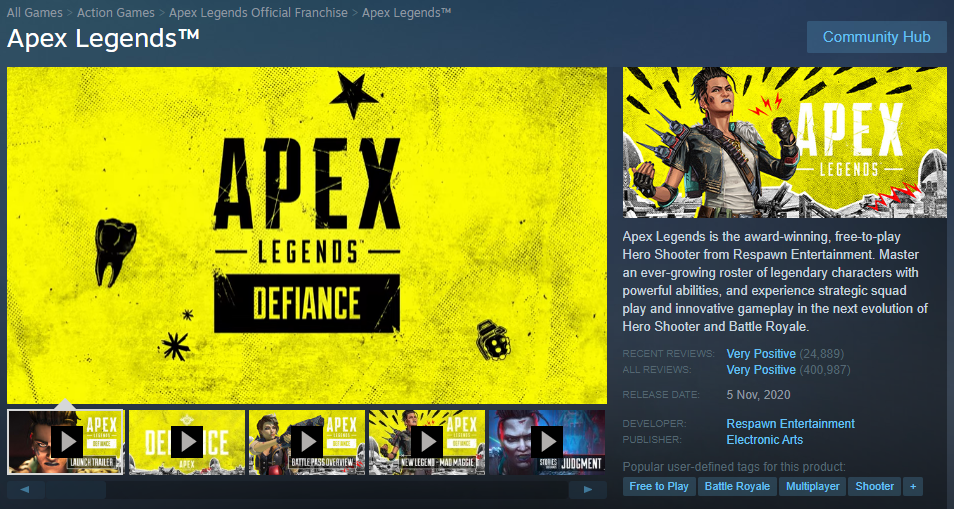
\includegraphics[scale=0.6]{figures/02_background/01_SteamStore_ApexLegends.png}
    \caption{A screenshot of the first section of the Steam store page for the game \textit{Apex Legends}\texttrademark~ \cite{SteamApexLegends}.}
    \label{fig:SteamStore_ApexLegends}
\end{figure}

\subsubsection{Reviews}

Users on Steam can provide reviews for games that they've purchased and played. A game review consists of a simple `thumbs up' or `thumbs down' rating, indicating that the user would or would not recommend the game to other users, as well as some written text. This review system differs from many other platforms which use numerical ratings, eg `out of ten' or `out of five'.

A game's store page will indicate a game's popularity using the percentage of user reviews that were positive (`thumbs up') both in total and over the last 30 days. These percentages are also attached to descriptions such as `Mixed' for a game with, for example, 50\% positive reviews and `Mostly Positive' for a game with 75\% positive reviews. There are also additional popularity descriptors for games with more than a certain number of total reviews. For example, a game with 96\% positive reviews but only 25 reviews in total would be described as `Positive' but a game with the same positive review percentage with 500 total reviews would be described as `Overwhelmingly Positive' \cite{SteamRatingsArticle}. A chart outlining this labelling system, seemingly based on \cite{SteamRatingsArticle}, is given in Figure \ref{fig:SteamStore_Ratings}.

\begin{figure}[ht]
    \centering
    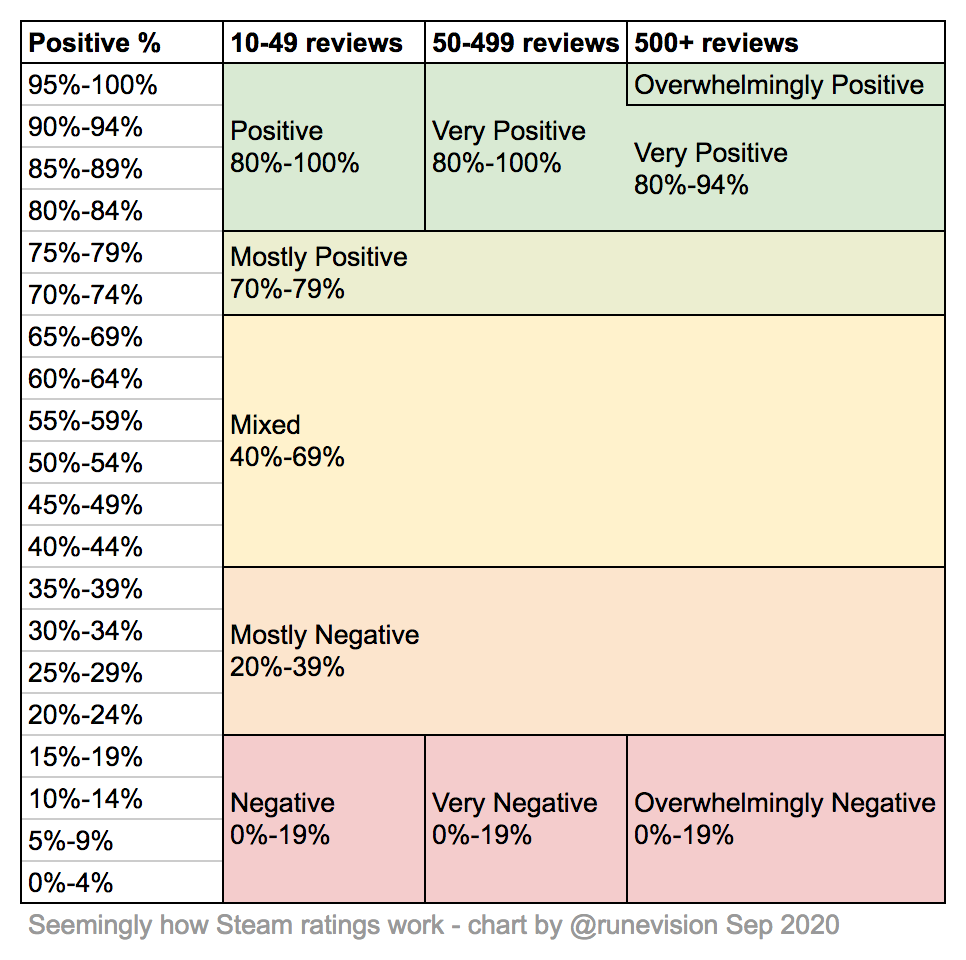
\includegraphics[scale=0.3]{figures/02_background/02_SteamStore_Ratings.png}
    \caption{Steam rating labels by positive review percentage and number of reviews \cite{SteamRatingsChart}.}
    \label{fig:SteamStore_Ratings}
\end{figure}

A certain number of selected reviews and recent reviews are included on a game's store page with an option provided for a user to browse all of that game's reviews on a separate page. Users can give other reviews a `thumbs up' if they found it helpful or a `thumbs down' if they did not, they can also mark a review as `funny' if they found it humorous. The selected reviews that appear on a game's store page are those reviews that received the most `helpful' ratings in the past 30 days.

\begin{figure}[ht]
    \centering
    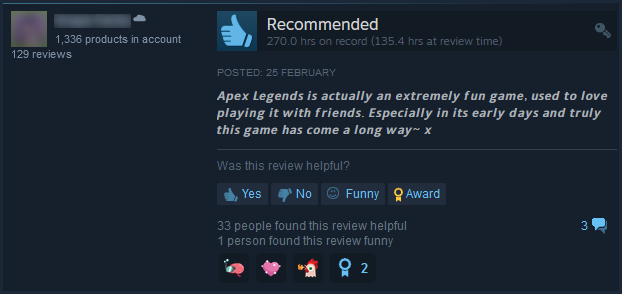
\includegraphics[scale=2.4]{figures/02_background/03_SteamStore_Review.png}
    \caption{A screenshot of a positive review for the game \textit{Apex Legends}\texttrademark~ \cite{SteamApexLegends}.}
    \label{fig:SteamStore_Review}
\end{figure}

As previously mentioned, a review consists of  a `thumbs up' or `thumbs down' rating as well as some written text. However, a review will also list the date that it was written, the amount of time that the user has played the game in total and at the time the review was written. The number of `helpful' and `funny' ratings the review received are also listed. Users can, at a later date, edit both the rating and text of their reviews and information about these edits, if any occurred, is also displayed. When writing a review a user can specify the language the review has been written in although it is not clear if this feature is always used. Finally, a review will also contain a link to the Steam profile of the reviewer as well as information about the number of games that the user owns and the number of reviews they've written. Other users can leave comments on reviews leading to nested discussion threads within the review system.

\subsection{Community} \label{sec:BG_Steam_Comm}

\subsubsection{Community Hubs}

Games on Steam also have what are referred to as `community hubs'. Within these hubs, users can create and participate in discussions on a forum and interact with other users in a chat room. They can also post and share artwork, screenshots and videos related to the game and publish in-game guides and tutorials. The developers of the game can also announce news and updates for their game within this hub. Certain games also support the sharing of game modifications, in-game items and other user-created content within the `Workshop' section of the hub.

\subsubsection{Groups}

Users can also create and join groups on Steam. These groups can be associated with a single game, numerous related games or no game at all. Groups can be discovered in a game's community hub or by using Steam's `find a group' search feature. Group administrators can control the privacy of their group by making them public, private or invite-only. Groups, like community hubs, have discussion forums and chat rooms and group administrators can schedule and host community events.

\subsection{Library} \label{sec:BG_Steam_Lib}

Once a user purchases a game it is added to their library. Users can organise, update or uninstall their games from inside of their library. A game's library page differs from its storefront page. From this page users can view which of their friends are currently playing or have played the game, browse a feed of news, patches and updates related to the game and see a list of in-game achievements and trading cards that they've unlocked. They can also write, edit and view their review of the game. The game's library page also provides direct access to sections of its community hub and there is a search feature present for finding groups related to the game.

\subsubsection{Achievements}

Achievements are rewards specified by a game's developers that are unlocked on Steam (outside of the game itself) usually upon completing particularly difficult sections of or tasking within a game.

\subsubsection{Trading Cards}

Trading cards are virtual items awarded to users in a somewhat random fashion as they play and progress through a particular game. Each game has a certain number of trading cards that users can collect and certain rewards are given to users upon collecting a game's full `set' of trading cards. By design, an individual user will not be able to collect every card on their own and will have to trade or purchase cards from other players of the game on a trading-specific market and forum. The rewards given to users upon completing a set of trading cards will be discussed in the sections that follow.

\subsection{User Profile} \label{sec:BG_Steam_Profile}

Each user has access to their own customisable Steam profile. Depending on the user in question's privacy settings, this profile can be viewed by any other user, their friends or nobody at all. Users can customise many aspects of their profile including their username, profile picture, location and a short description of themselves. A profile can be used to showcase, among other things, which games the user has played or what in-game achievements they have earned. Other users can also leave comments on a user's profile page.

Users can earn `experience points' on Steam in order to increase their profile's `level'. This level is displayed on the user's profile and, as a user increases in level, they get access to additional ways to customise their profile. Experience points are gained by completing sets of trading cards, as discussed in the previous section, by purchasing and playing additional games and by simply maintaining their Steam account for long periods of time.

\subsubsection{Friends}

Users can add other users as friends on Steam. Unlike other social networks such as Twitter, a Steam friendship is bidirectional and a friend request must be accepted by the other party before users are considered friends. The number of friends a user can have is initially limited to 250 but this cap is increased by five each time the user gains another level on Steam.

If two users are friends they can send direct messages to each other, invite each other to games that support multiplayer and view each other's in-game activity.

\section{The Dataset} \label{sec:BG_Dataset}

The dataset used in this project was gathered by Professor Douglas Leith at Trinity College Dublin using a custom-built web scraper written in Python that uses the Scrapy library. The dataset contains comprehensive review, friendship and group membership data for a large number of Steam users. Data is stored using the JSON Lines format where each line or entry in a data file contains a single record, eg a single user's friend data, stored in the form of a JSON object. In its raw form, the dataset contains almost 23 GB of data.

The dataset is split into four parts: reviews, review texts, friends and groups. The review data contains information about all of the reviews left by a particular user excluding the actual text of the review. The review text data contains the corresponding text data for all of the aforementioned users and reviews. The friend data contains a list of all of the friends a particular user has while the group data contains a list of all of the groups the user is a member of.

In total, the dataset contains full review, friendship and group membership data for 4,000,033 individual users. All users in the dataset without at least one review and one friend are excluded in the aforementioned count and in all later work.

\subsection{Steam User IDs} \label{sec:BG_Dataset_UIDs}

Every user on Steam is given a unique user ID in the form of a 17 digit number. The URL that leads to a user's profile relies on this user ID as opposed to, for example, their username. In the case of our dataset, and potentially across Steam as a whole, only the final nine digits of a user's ID appear to vary from user to user while the first eight digits remain constant. These URLs are formatted like so:  \texttt{https://steamcommunity.com/profiles/76561198XXXXXXXXX}. Throughout the dataset, users are identified by the \texttt{profiles/76561198XXXXXXXXX} section of their profile URL.

\subsection{Reviews} \label{sec:BG_Dataset_Revs}

Each entry in this section of the dataset contains an indicator that the entry concerns review data, the Steam user ID for the user in question as well as an array containing data for each of the reviews they've left. Each of the entries in the review array contains the following information:

\begin{itemize}
    \item the unique ID of the game being reviewed;
    \item the polarity of the review (`thumbs up' or `thumbs down');
    \item whether or not the review was for an early access game;
    \item the number of hours the user has played the game in total;
    \item the number of hours the user had played the game when the review was written;
    \item the date (as a string) that the review was written as well as the corresponding Unix timestamp;
    \item if the review was later edited by the user: the date and timestamp that the editing occurred;
    \item the number of `helpful' votes the review received;
    \item the number of `funny' votes the review received; and
    \item the user-specified language that the review was written in.
\end{itemize}

An example entry can be seen in Listing \ref{lst:ExampleData_Review}.

\lstinputlisting[caption={An example of review data for a user with a single written review.},captionpos=b,label={lst:ExampleData_Review}]{listings/02_background/ExampleData_Review.json}

\subsection{Review Texts} \label{sec:BG_Dataset_Texts}

As was the case with the reviews data, each entry in this section contains an indicator that the entry concerns review text data, the Steam user ID of the user in question and an array containing data for each of the user's reviews. Each entry in this array contains the unique ID of the game being reviewed and the review's text content. An example entry can be seen in Listing \ref{lst:ExampleData_ReviewText}.

\lstinputlisting[caption={An example of review text data for a user with a single written review.},captionpos=b,label={lst:ExampleData_ReviewText}]{listings/02_background/ExampleData_ReviewText.json}

\subsection{Friends} \label{sec:BG_Dataset_Friends}

Each entry in this section contains an indicator that the entry concerns friend data, the Steam user ID of the user in question and an array consisting of the user IDs of all of their friends. An example entry can be seen in Listing \ref{lst:ExampleData_Friend}.

\lstinputlisting[caption={An example of friend data for a user with two friends.},captionpos=b,label={lst:ExampleData_Friend}]{listings/02_background/ExampleData_Friend.json}

\subsection{Groups} \label{sec:BG_Dataset_Groups}

Each entry in this section contains an indicator that the entry concerns group data, the Steam user ID of the user in question and an array consisting of the Steam community URLs for each of the groups the user is a member of. An example entry can be seen in Listing \ref{lst:ExampleData_Group}.

\lstinputlisting[caption={An example of group data for a user who is a member of two groups.},captionpos=b,label={lst:ExampleData_Group}]{listings/02_background/ExampleData_Group.json}

\subsection{Conversion to CSV} \label{sec:BG_Dataset_CSV}

To make the data easier to work with in Python they were converted from the JSON Lines format into the CSV format.

\subsubsection{Reviews and Texts}

Steam user IDs were mapped to unique integers counting up from zero and these new IDs were applied to both the friend and group data, too. The review texts and other features were combined into a single row. A sample row of the converted review data is given in Table \ref{tab:ExampleData_Review} while the meanings of the column names are given in Table \ref{tab:ExampleData_Review_Abrv}.

\begin{table}[ht]
    \centering
    \begin{tabular}{l l}
        \toprule
        \textbf{Acronym} & \textbf{Meaning} \\\midrule
        UID & User ID\\
        GID & Game ID\\
        P & Polarity (voted up)\\
        EA & Early access\\
        PT & Playtime in total\\
        PR & Playtime at review\\
        TC & Timestamp at creation\\
        TU & Timestamp at update\\
        VU & Votes up\\
        VF & Votes funny\\
        \bottomrule\\
    \end{tabular}
    \caption{Acronyms for converted review column names.}
    \label{tab:ExampleData_Review_Abrv}
\end{table}

\begin{table}[ht]
    \centering
    \begin{tabular}{l l l l l l l l l l l}
        \toprule
        \textbf{UID} & \textbf{GID} & \textbf{P} & \textbf{EA} & \textbf{PT} & \textbf{PR} & \textbf{TC} & \textbf{TU} & \textbf{VU} & \textbf{VF} & \textbf{Text} \\\midrule
        1 & 12 & 1 & 0 & 3.4 & 2.2 & 1649089205 & 1649089205 & 3 & 0 & "Good game"\\
        \bottomrule\\
    \end{tabular}
    \caption{An example of converted review data.}
    \label{tab:ExampleData_Review}
\end{table}

\subsubsection{Friends}

A sample row from the converted friend data is given in Table \ref{tab:ExampleData_Friend}.

\begin{table}[ht]
    \centering
    \begin{tabular}{l l}
        \toprule
        \textbf{User ID} & \textbf{Friend IDs} \\\midrule
        1 & $2,3,4,5$\\
        \bottomrule\\
    \end{tabular}
    \caption{An example of converted friend data.}
    \label{tab:ExampleData_Friend}
\end{table}

\subsubsection{Groups}

Group names were mapped to unique integers counting up from zero. A sample row of the converted group data is given in Table \ref{tab:ExampleData_Group}.

\begin{table}[ht]
    \centering
    \begin{tabular}{l l}
        \toprule
        \textbf{User ID} & \textbf{Group IDs} \\\midrule
        1 & $2,3,4,5$\\
        \bottomrule\\
    \end{tabular}
    \caption{An example of converted group data.}
    \label{tab:ExampleData_Group}
\end{table}

\chapter{Dataset Examination} \label{sec:Dataset}

\section{Friends} \label{sec:Dataset_Friends}

The number of friends users in the dataset have can be seen in Figure \ref{fig:Dataset_HistFriends}. Outliers\footnote[2]{Values outside of the interquartile range multiplied by some scaling value were considered to be outliers \cite{Seo2006_Outliers}. The scaling value was chosen so as to balance visual and statistical clarity.} have been excluded from the aforementioned histogram for the sake of visual clarity and, as such, users with more than 119 friends, 2\% of all users, are not shown. The mean number of friends users have is 28.7 (\textit{SD} = 46.9) and the median is 16. As mentioned in section \ref{sec:BG_Dataset}, users without any friends have been excluded.

Users in the dataset tend to have a modest number of friends with 75\% of users having 7 or more friends, although users with a single friend are the most common occurrence.

\begin{figure}[ht]
    \centering
    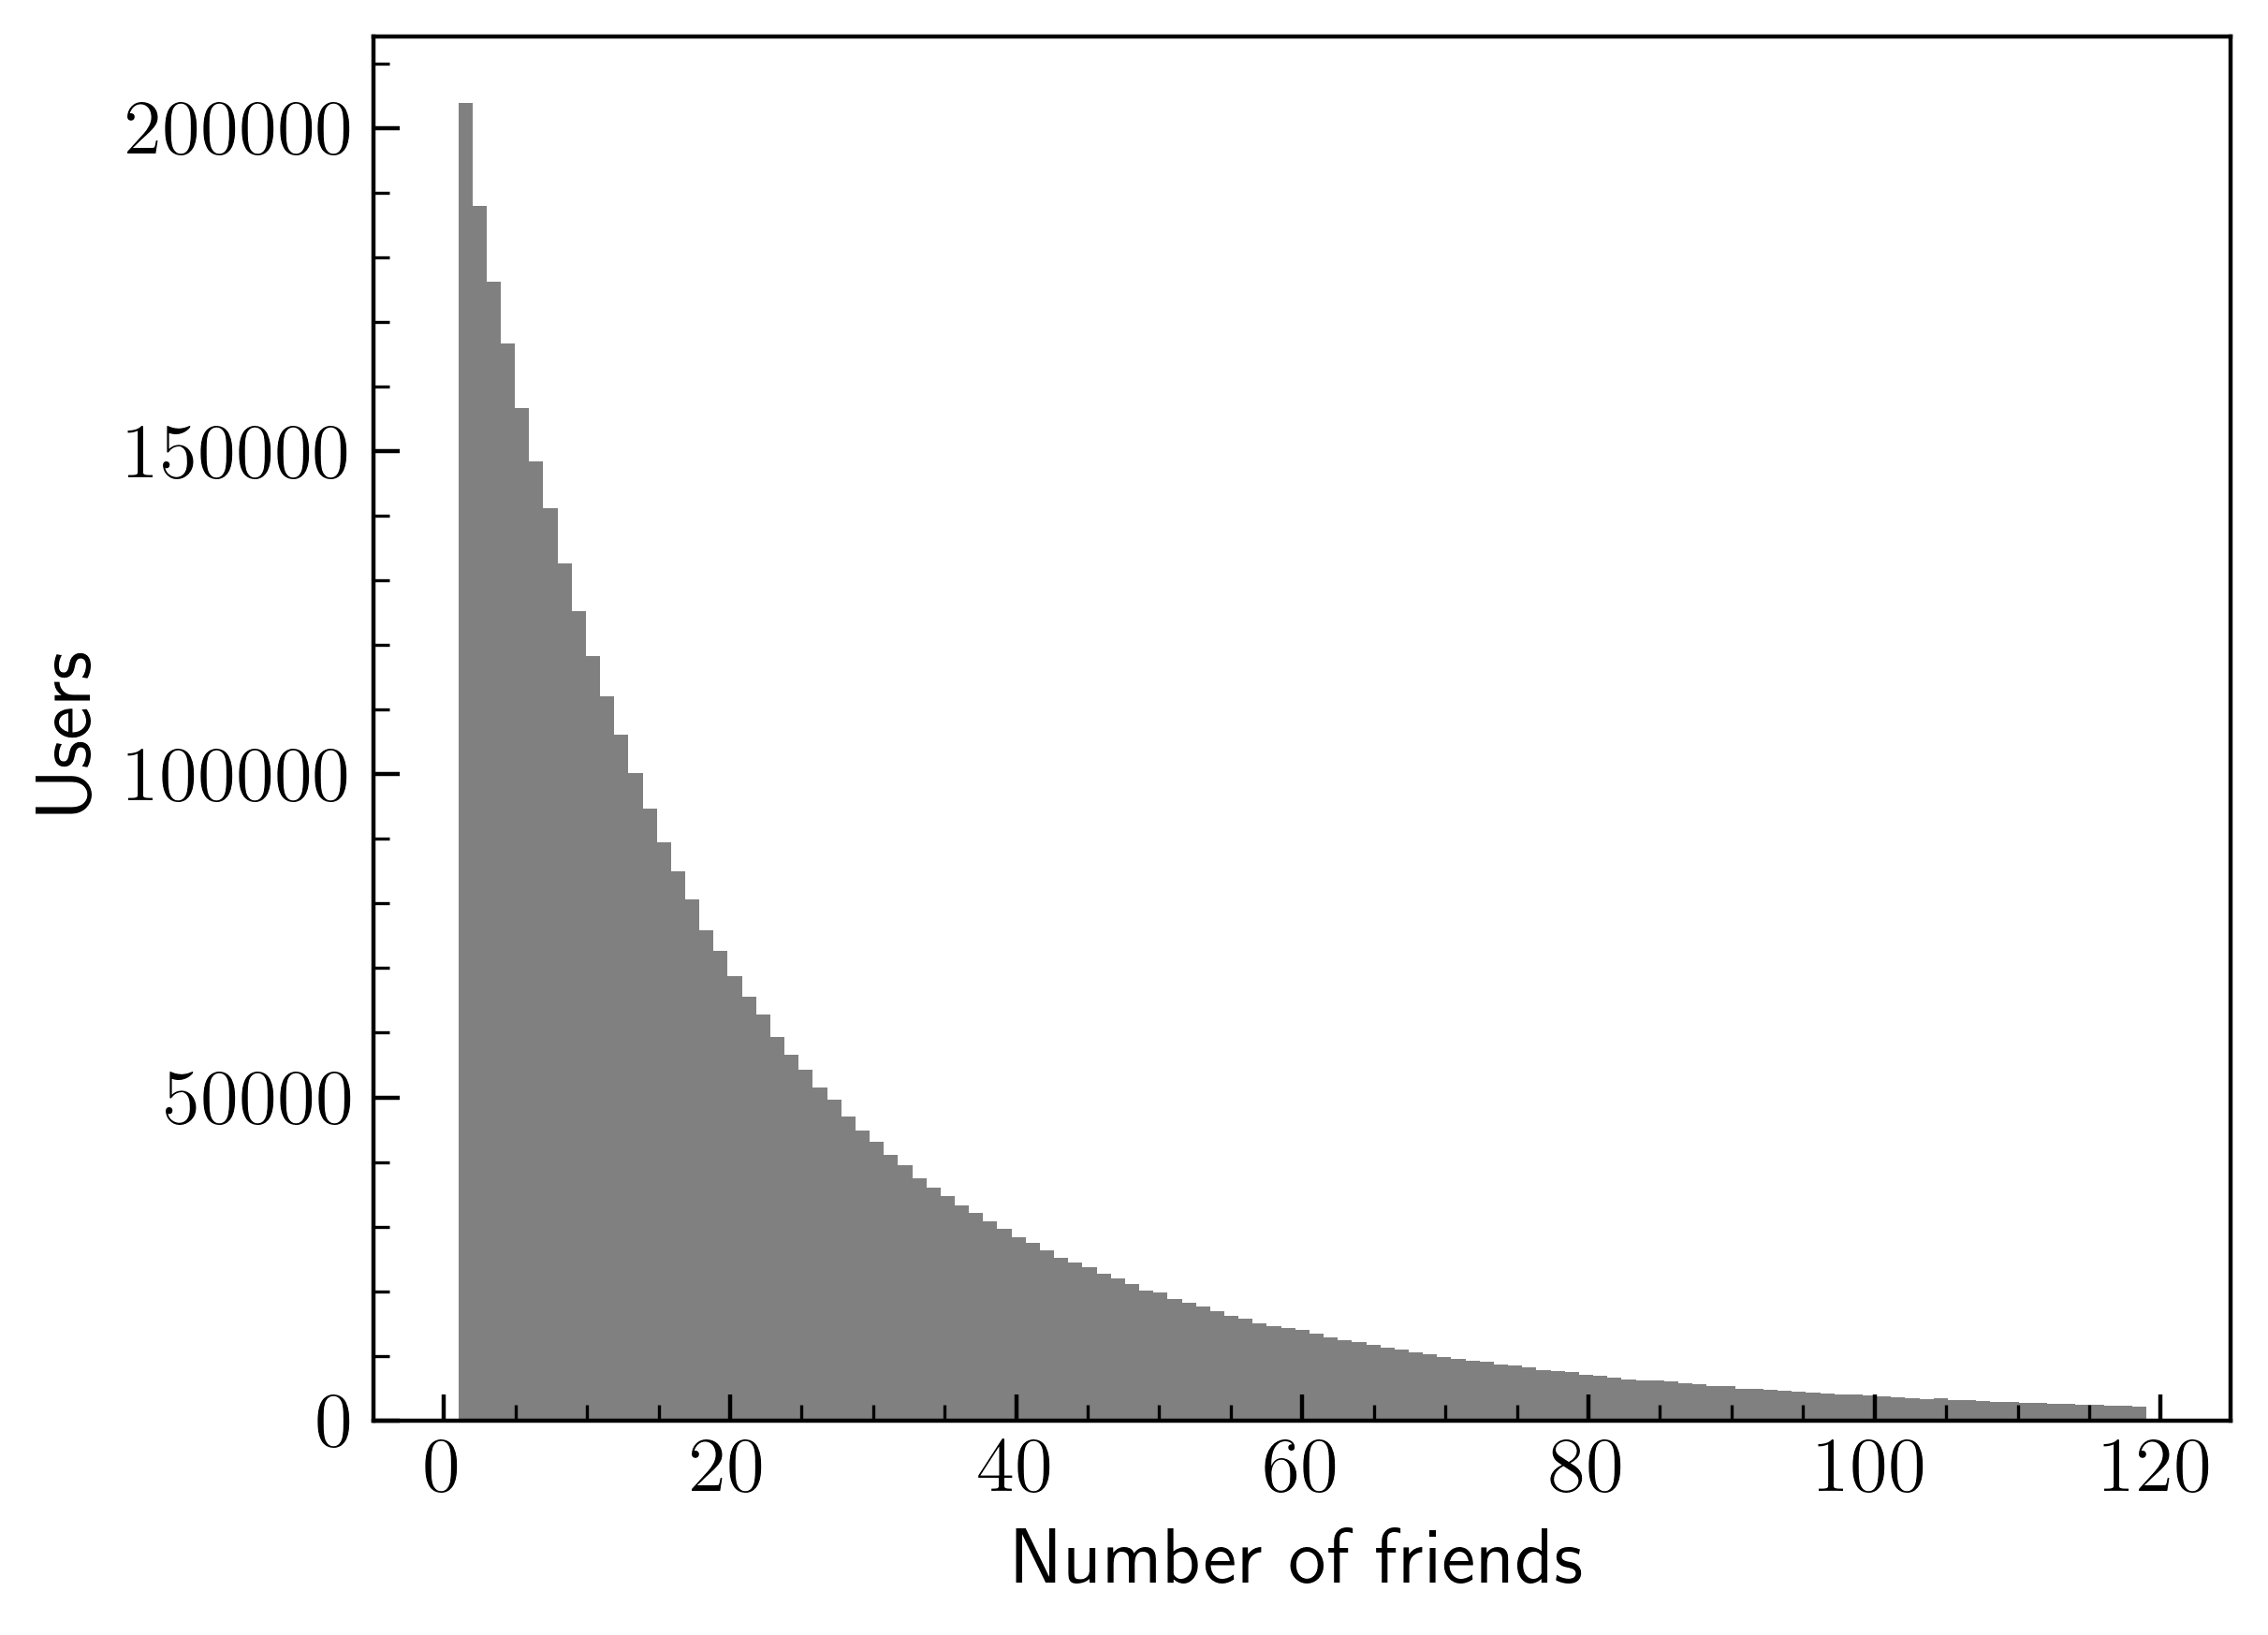
\includegraphics[scale=0.55]{figures/03_dataset/01_hist_friends.png}
    \caption{Number of friends that users have.}
    \label{fig:Dataset_HistFriends}
\end{figure}

\section{Groups} \label{sec:Dataset_Groups}

The number of members groups in the dataset have as well as the number of groups users are members of can be seen in Figure \ref{fig:Dataset_HistsGroups}. Groups with more than 12 members, 5\% of all groups, and users who are members of more than 45 groups, 5\% of all users, have been excluded from their respective histograms. The mean number of members groups have is 8.9 (\textit{SD} = 339.2) and the median is 1. The mean number of groups users are members of is 12.8 (\textit{SD} = 37.2) and the median is 4. Due to the nature in which the data was gathered, the values given for the number of members that groups have is limited to those users included in the dataset as opposed to all users on Steam.

The majority of groups in the dataset only contain a single member and most users tend not to be members of many, if any, groups.

\begin{figure}[ht]
    \centering
    \begin{subfigure}[ht]{0.49\textwidth}
        \centering
        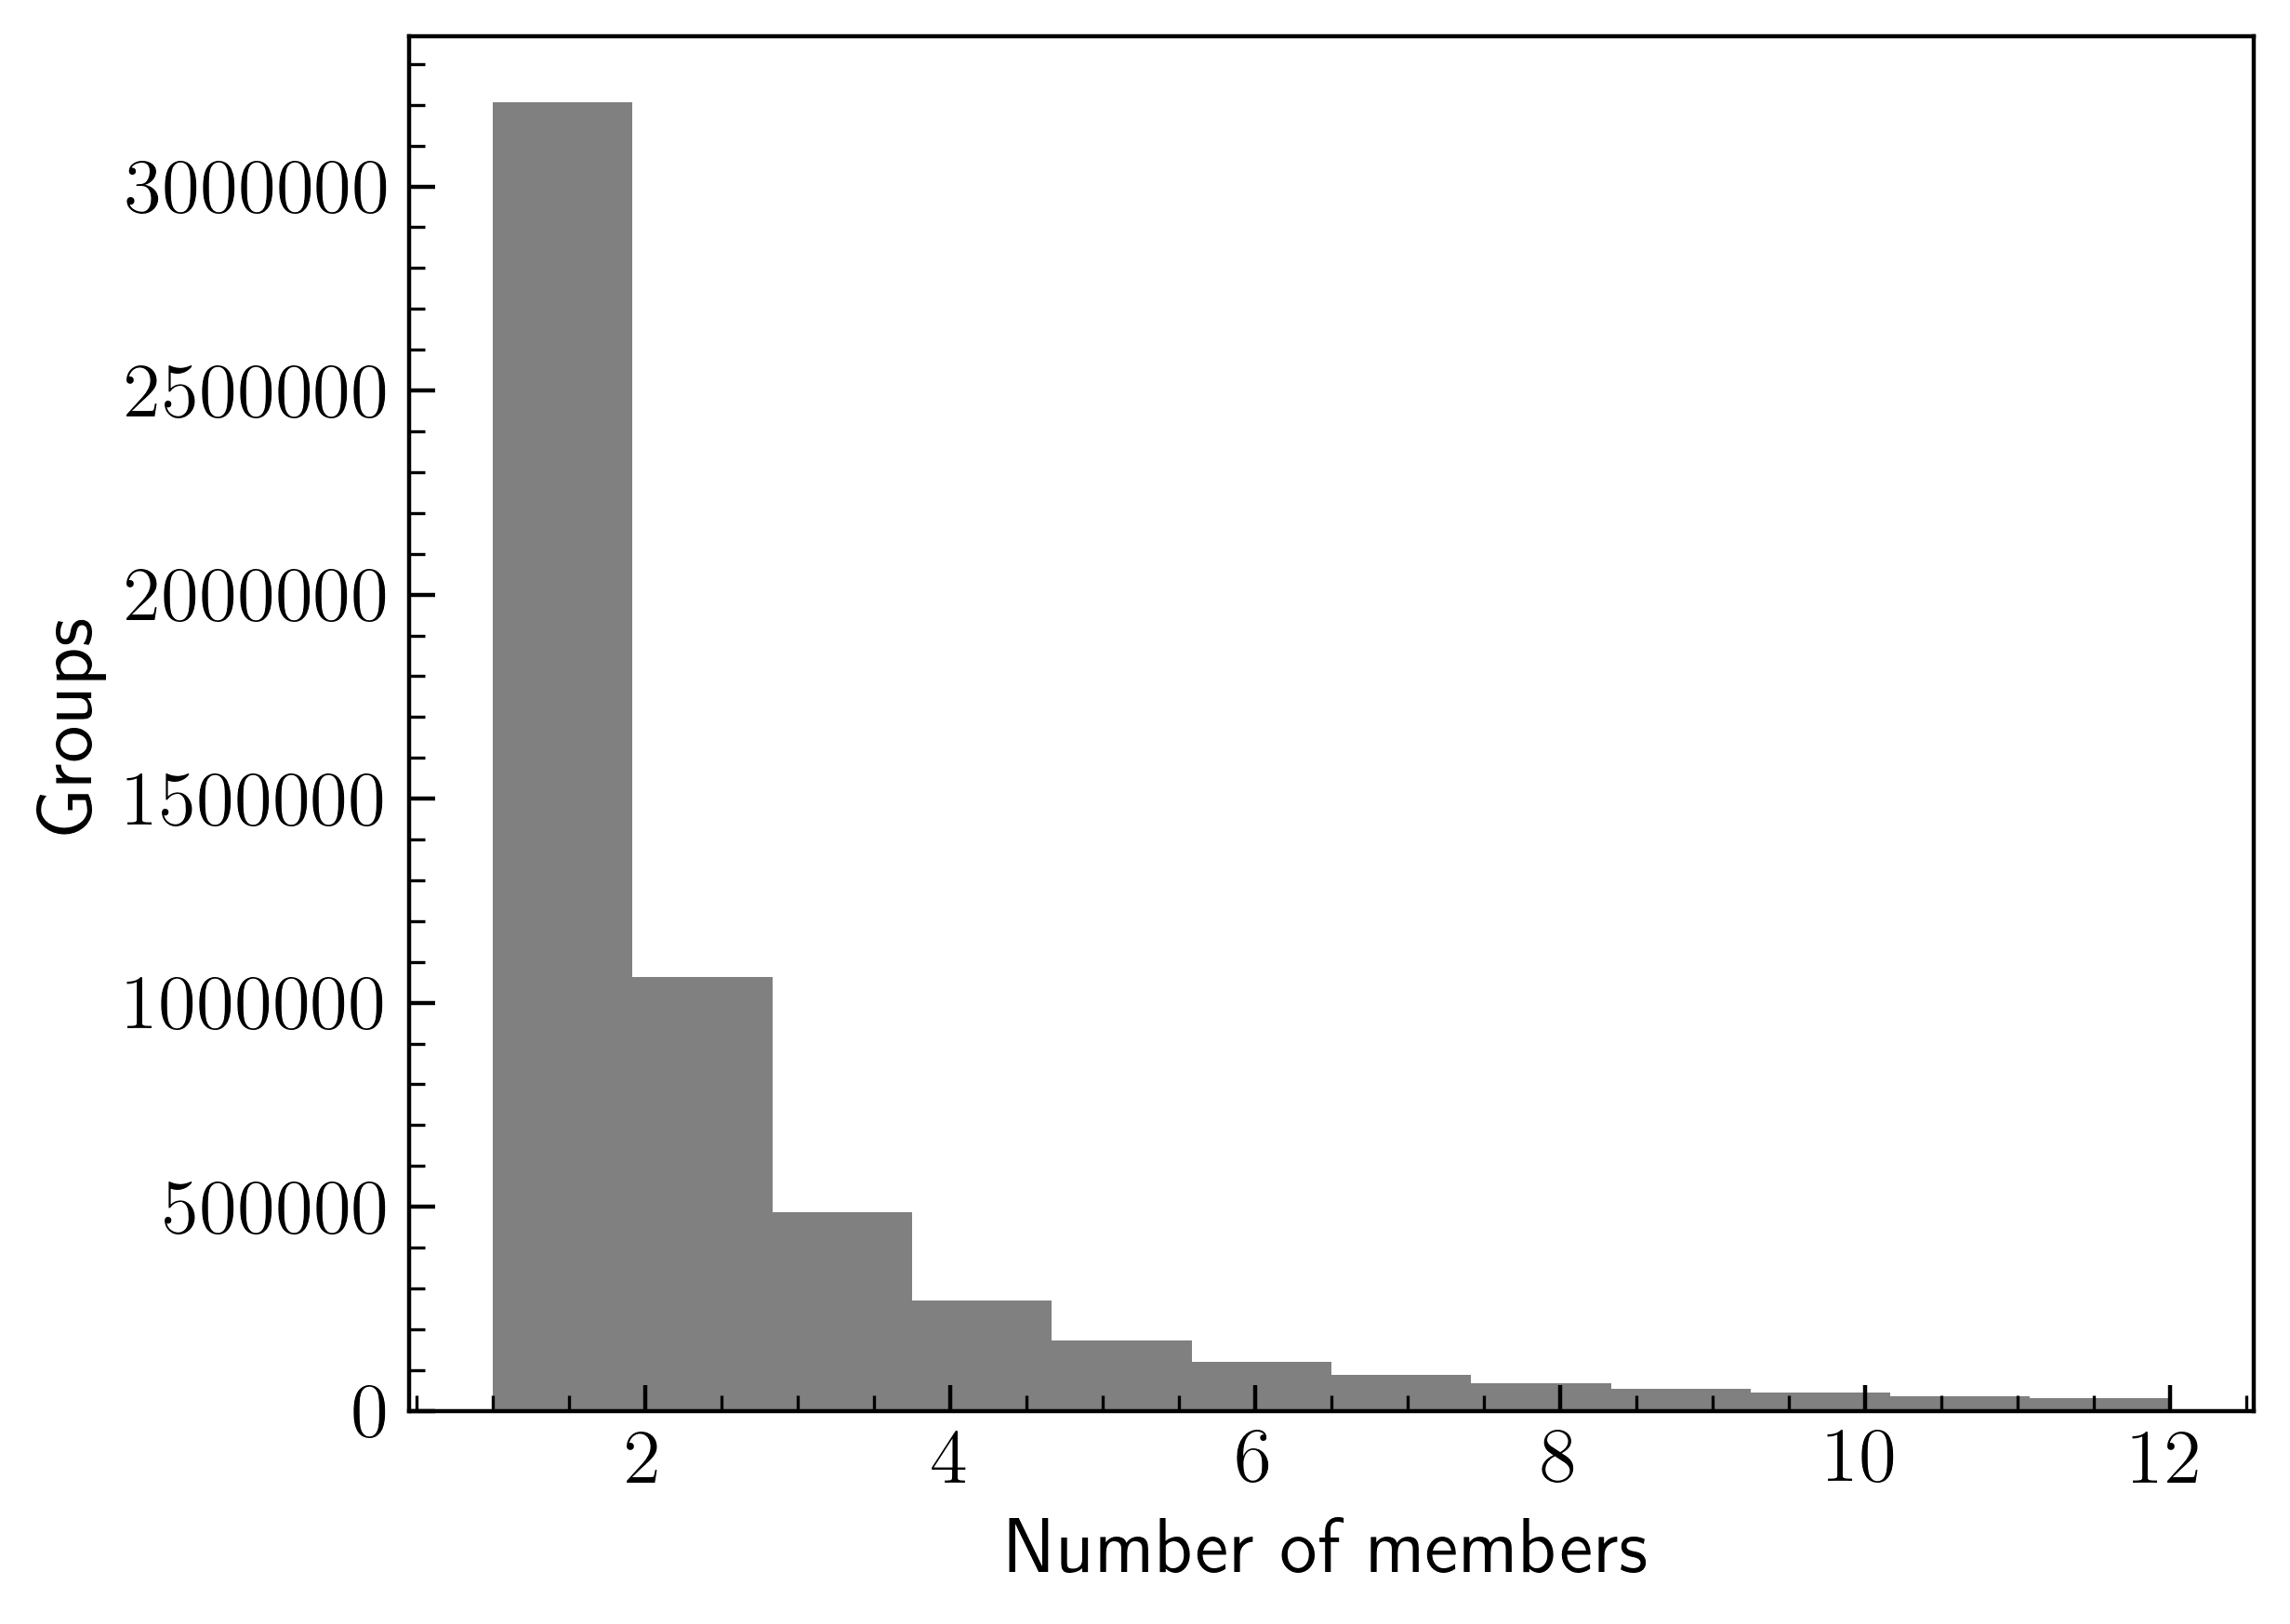
\includegraphics[width=\textwidth]{figures/03_dataset/02_hist_group_users.png}
        \caption{Number of members that groups have.}
        \label{fig:Dataset_HistGroupUsers}
    \end{subfigure}
    \hfill
    \begin{subfigure}[ht]{0.49\textwidth}
        \centering
        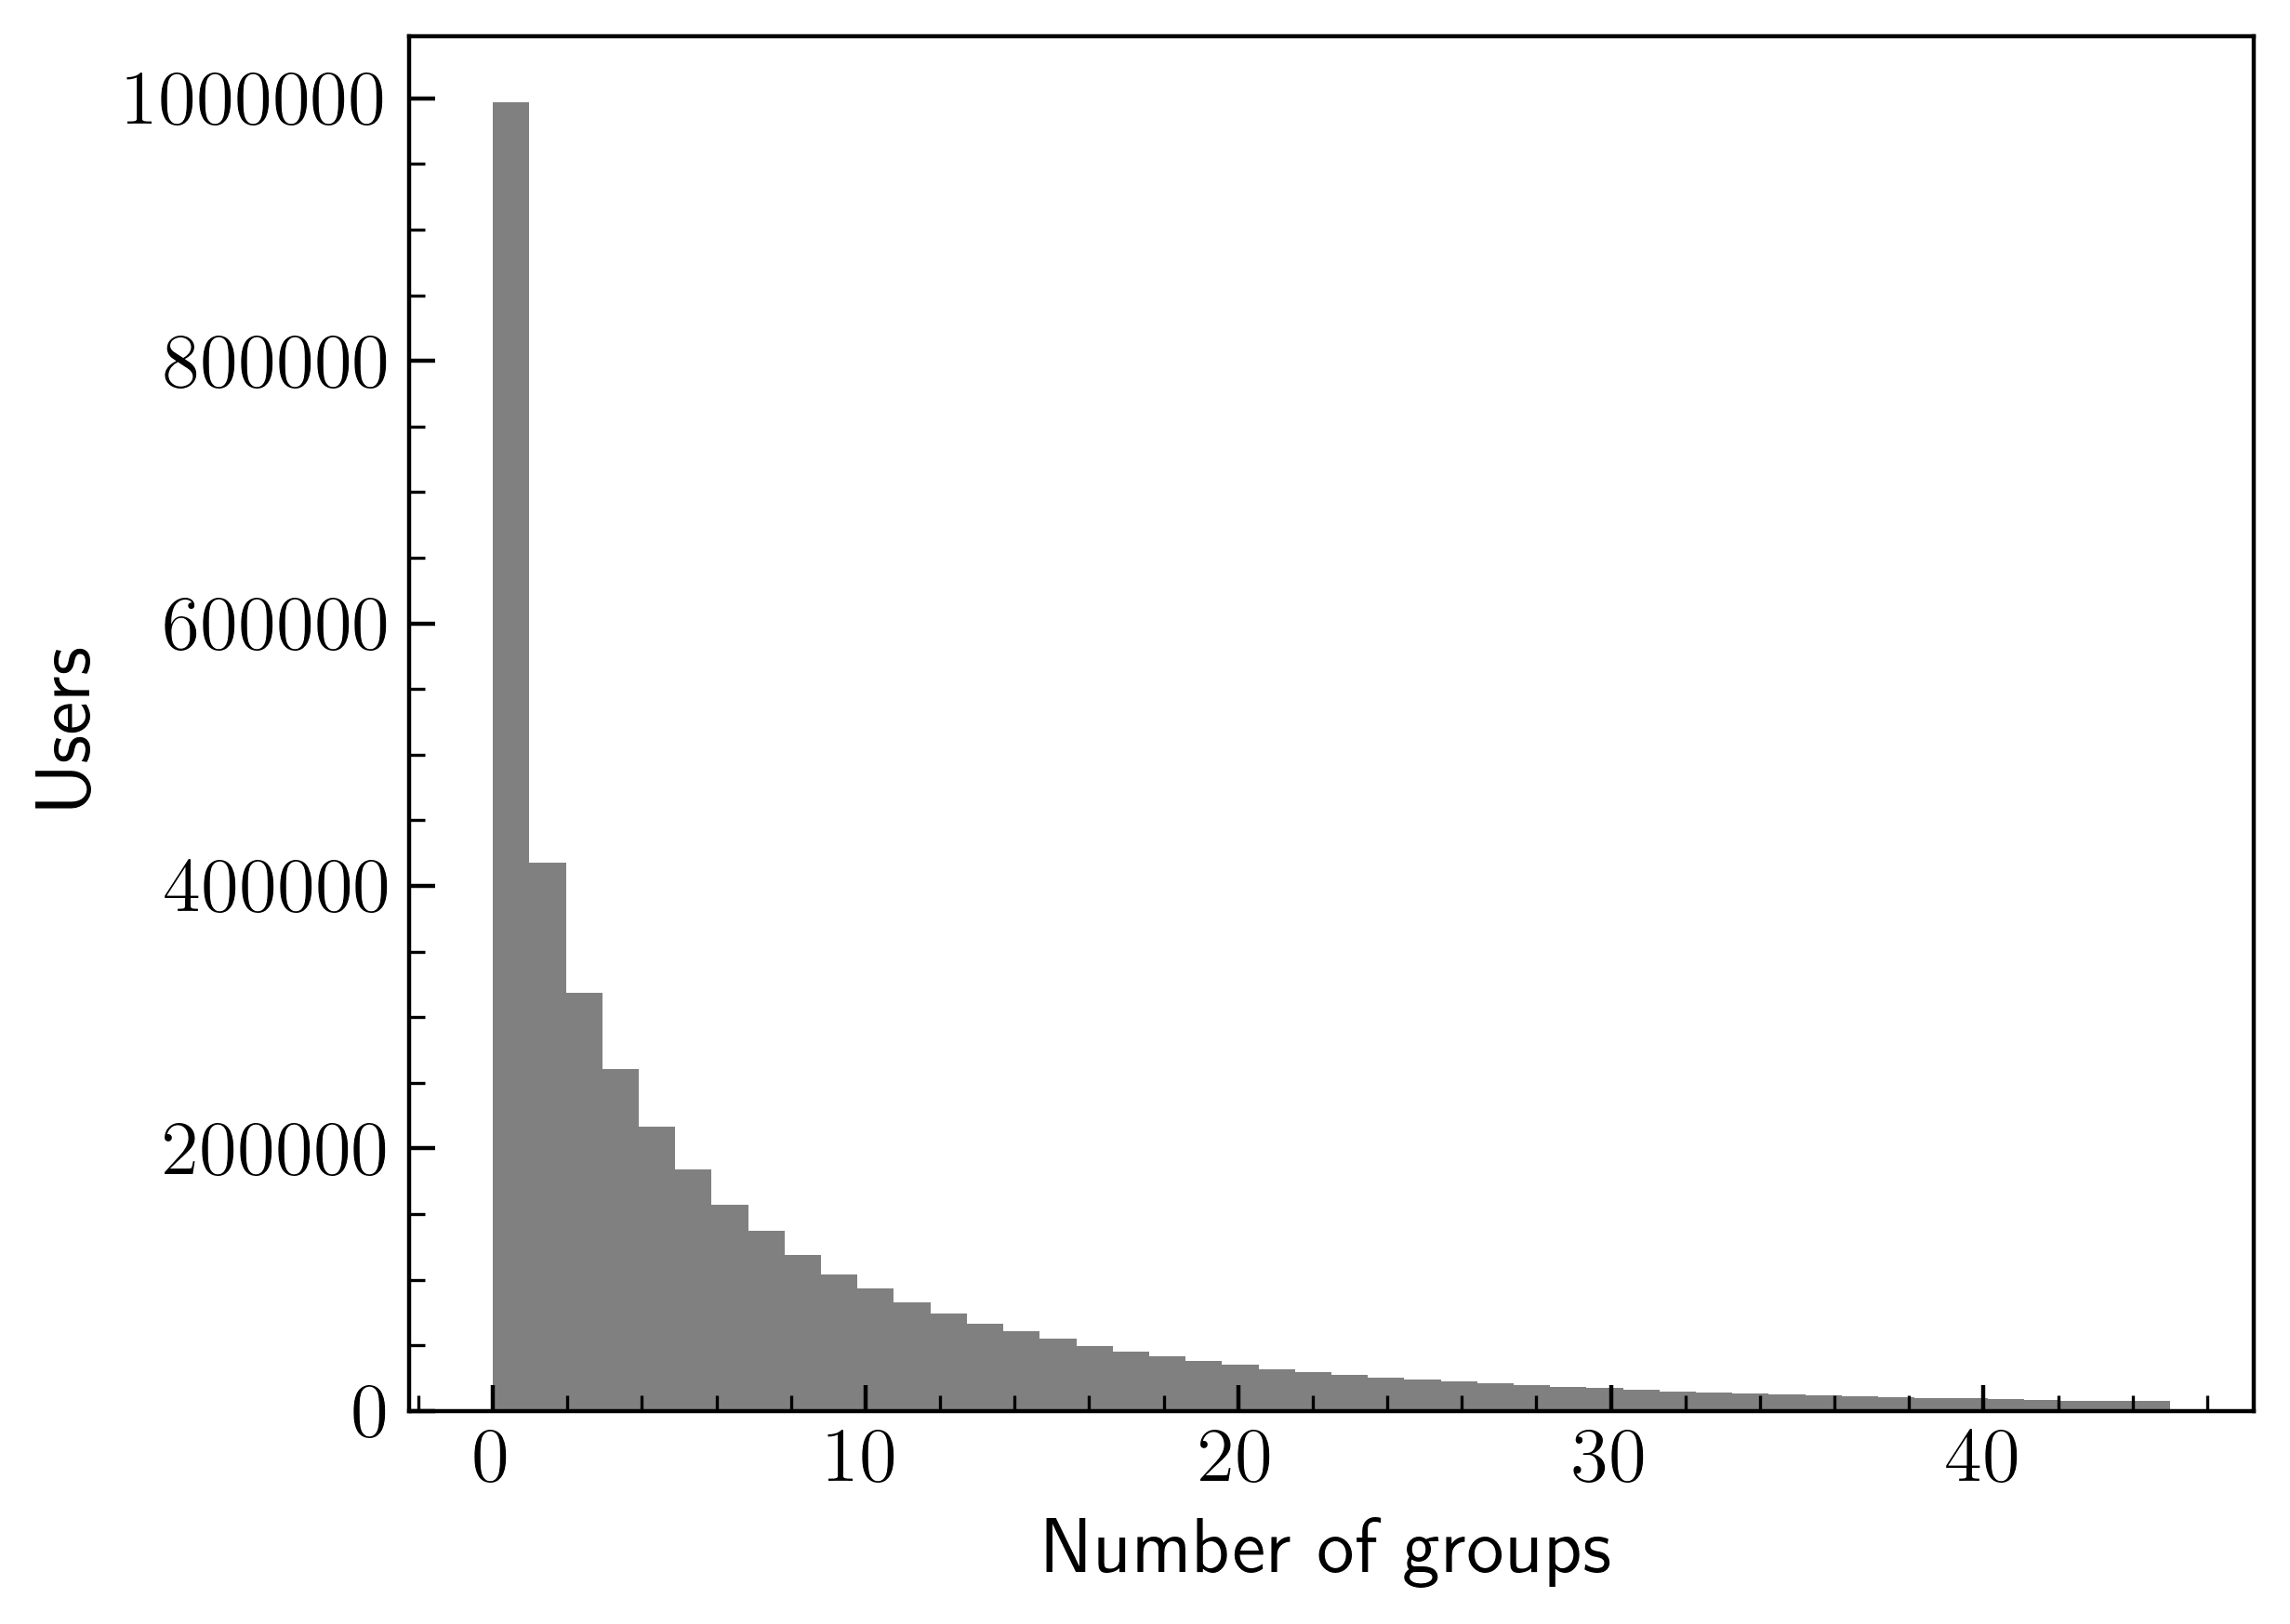
\includegraphics[width=\textwidth]{figures/03_dataset/03_hist_user_groups.png}
        \caption{Number of groups that users are members of.}
        \label{fig:Dataset_HistUserGroups}
    \end{subfigure}
    \caption{Group membership distributions.}
    \label{fig:Dataset_HistsGroups}
\end{figure}

\section{Reviews} \label{sec:Dataset_Reviews}

\subsection{Number of Reviews}

The number of reviews users have written as well as the number of reviews that games have can be seen in Figure \ref{fig:Dataset_HistsReviews}. Users who have written more than 22 reviews, 3\% of all users, and games with more than 161 reviews, 8\% of all games, have been excluded from their respective histograms. The mean number of reviews users have written is 4.6 (\textit{SD} = 16.8) and the median is 2. The mean number of reviews games have is 165.5 (\textit{SD} = 3611.1) and the median is 7. As was the case with groups, the values given for the number of reviews that games have is limited to those reviews included in the dataset as opposed to all reviews on Steam.

Most users in the dataset have only written a single review and 75\% of users have written 4 reviews or fewer. Similarly, most games in the dataset have only had a single review written for them.

\begin{figure}[ht]
    \centering
    \begin{subfigure}[ht]{0.49\textwidth}
        \centering
        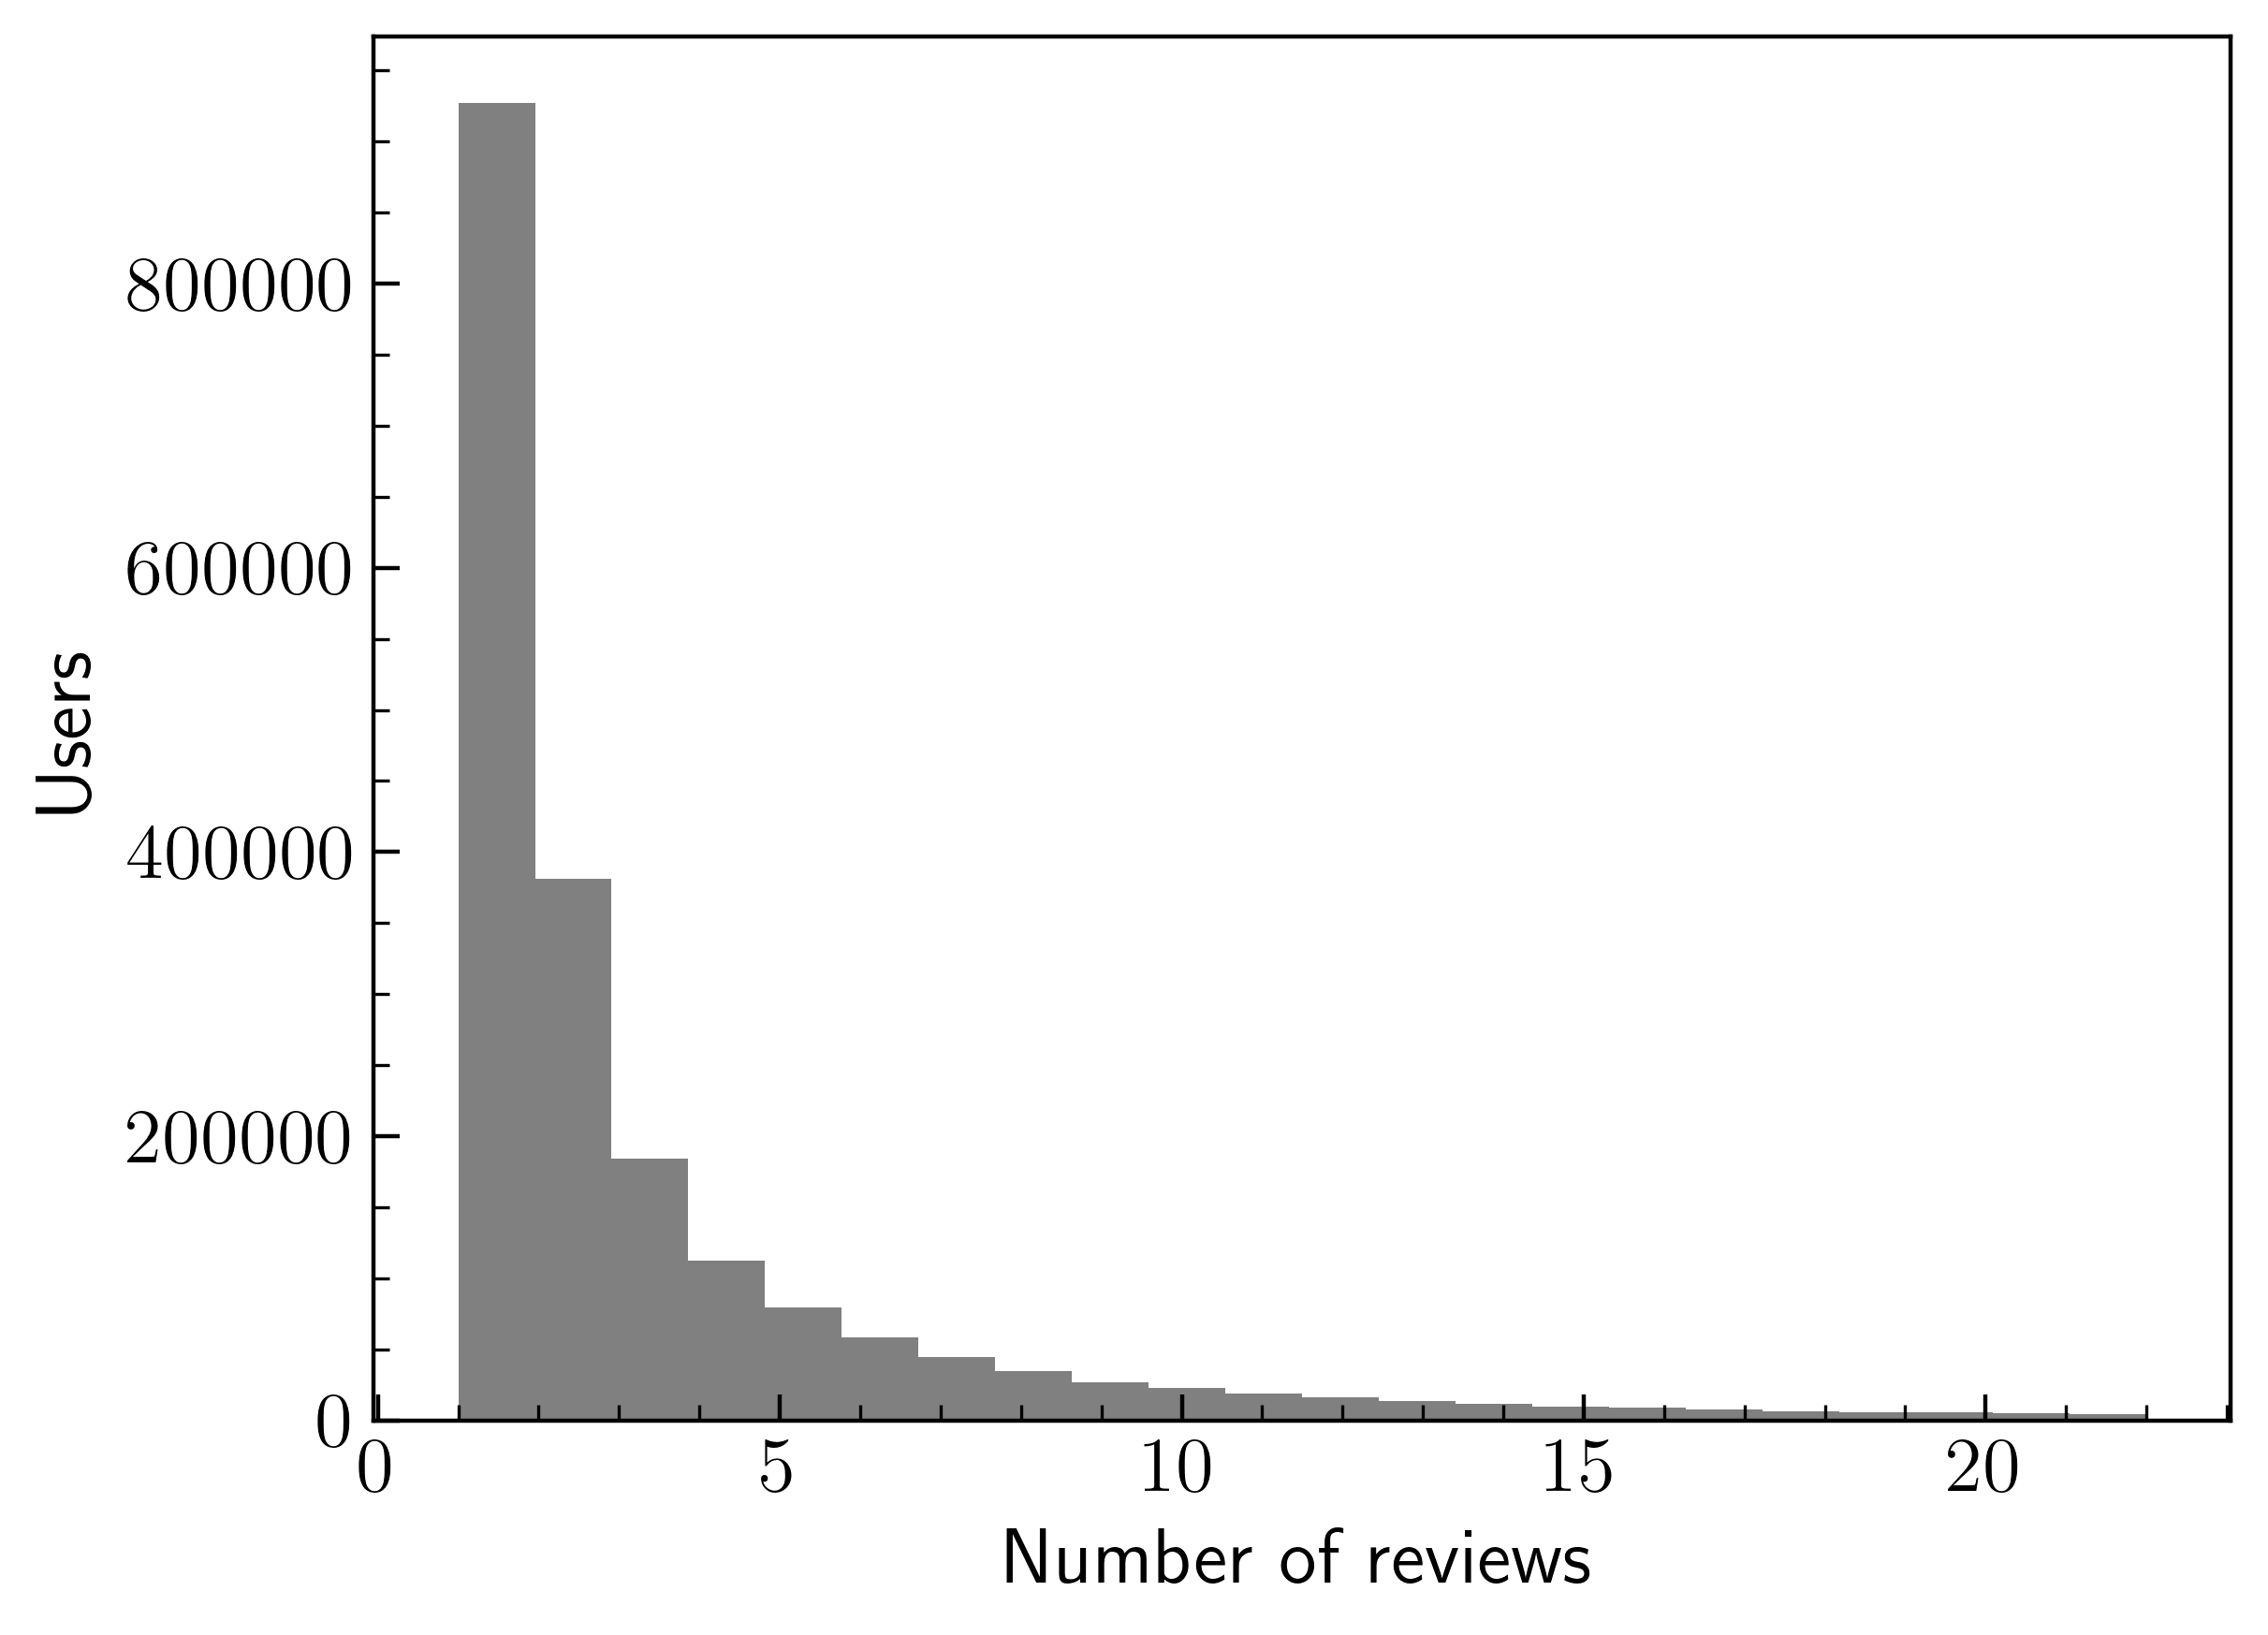
\includegraphics[width=\textwidth]{figures/03_dataset/04_hist_user_reviews.png}
        \caption{Number of reviews users wrote.}
        \label{fig:Dataset_HistUserReviews}
    \end{subfigure}
    \hfill
    \begin{subfigure}[ht]{0.49\textwidth}
        \centering
        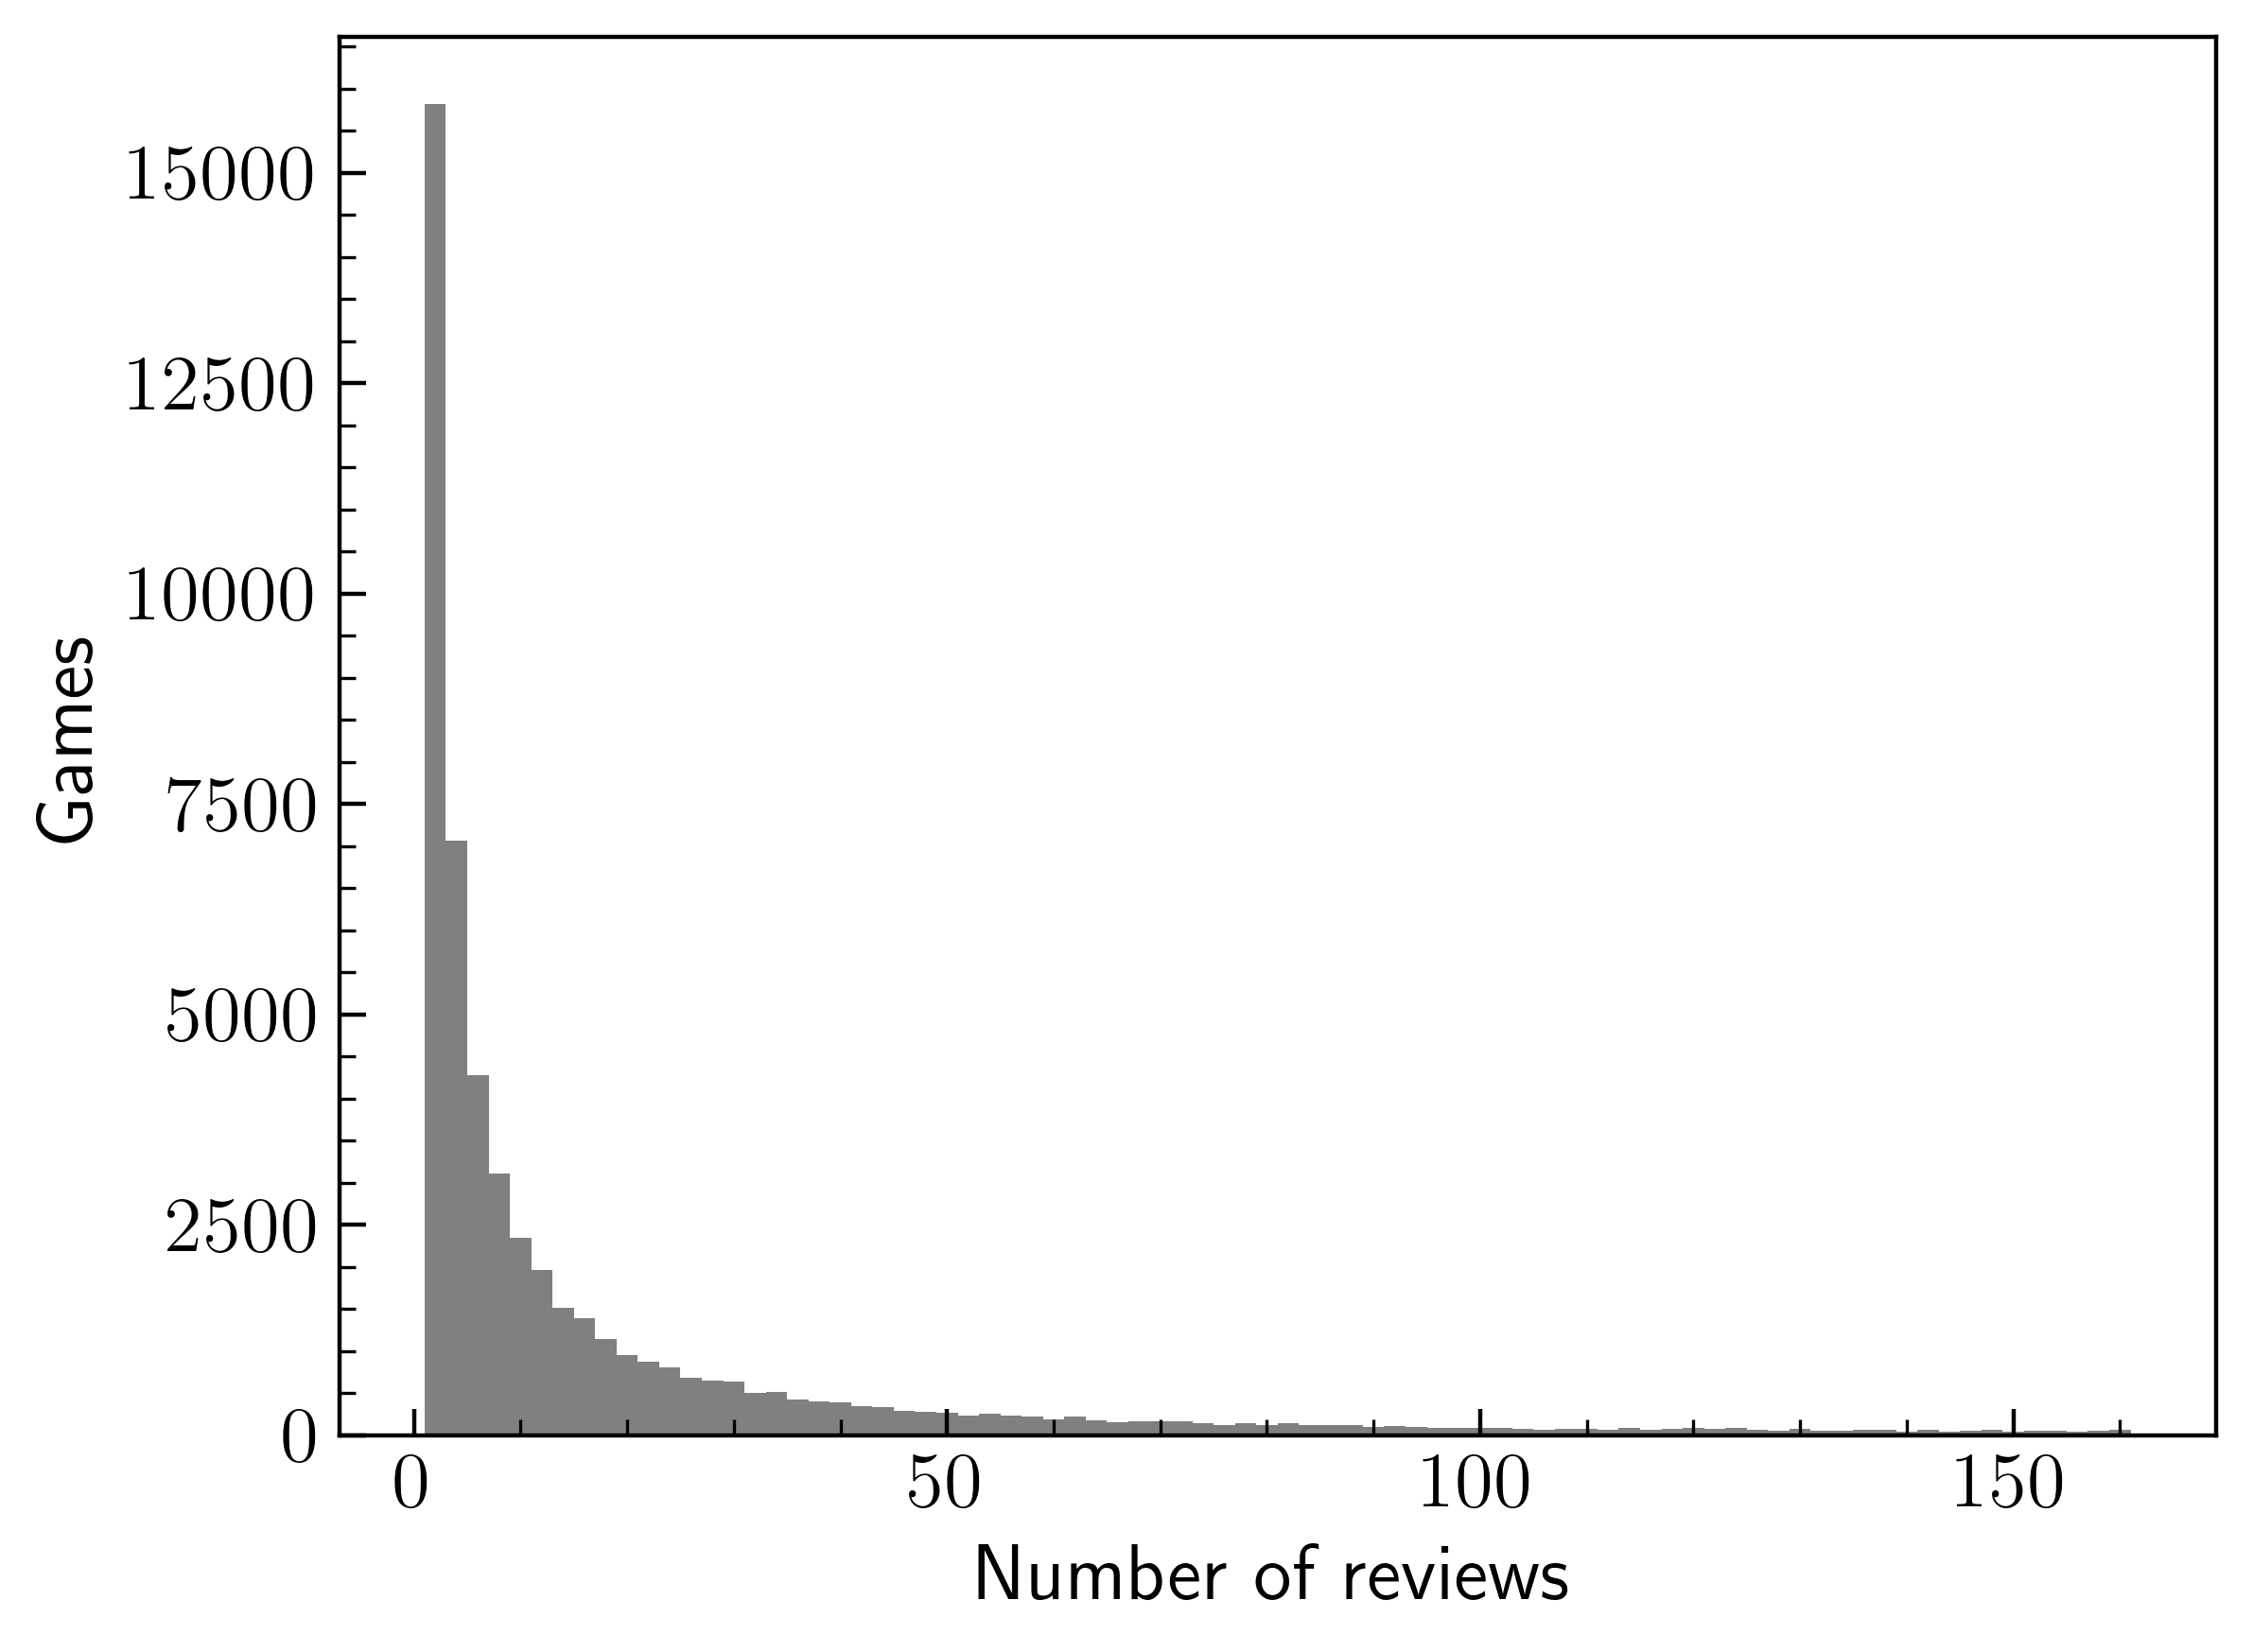
\includegraphics[width=\textwidth]{figures/03_dataset/05_hist_game_reviews.png}
        \caption{Number of reviews left for games.}
        \label{fig:Dataset_HistGameReviews}
    \end{subfigure}
    \caption{Review count distributions.}
    \label{fig:Dataset_HistsReviews}
\end{figure}

\subsection{Polarities}

The distribution of users based on the proportion of their reviews that are positive can be seen in Figure \ref{fig:Dataset_HistsPolarities}. When all users are considered, the mean positive proportion is 88.5\% (\textit{SD} = 25.2\%) and the median is 100\%. When only users who have written at least five reviews are considered, the mean positive proportion is 85.8\% (\textit{SD} = 16.5\%) and the median is 90\%.

When all users are considered the vast majority of users have a positive proportion of 100\%. The distribution becomes a little more balanced when only users with five or more reviews are considered although it still skews strongly to the right.

\begin{figure}[ht]
    \centering
    \begin{subfigure}[ht]{0.49\textwidth}
        \centering
        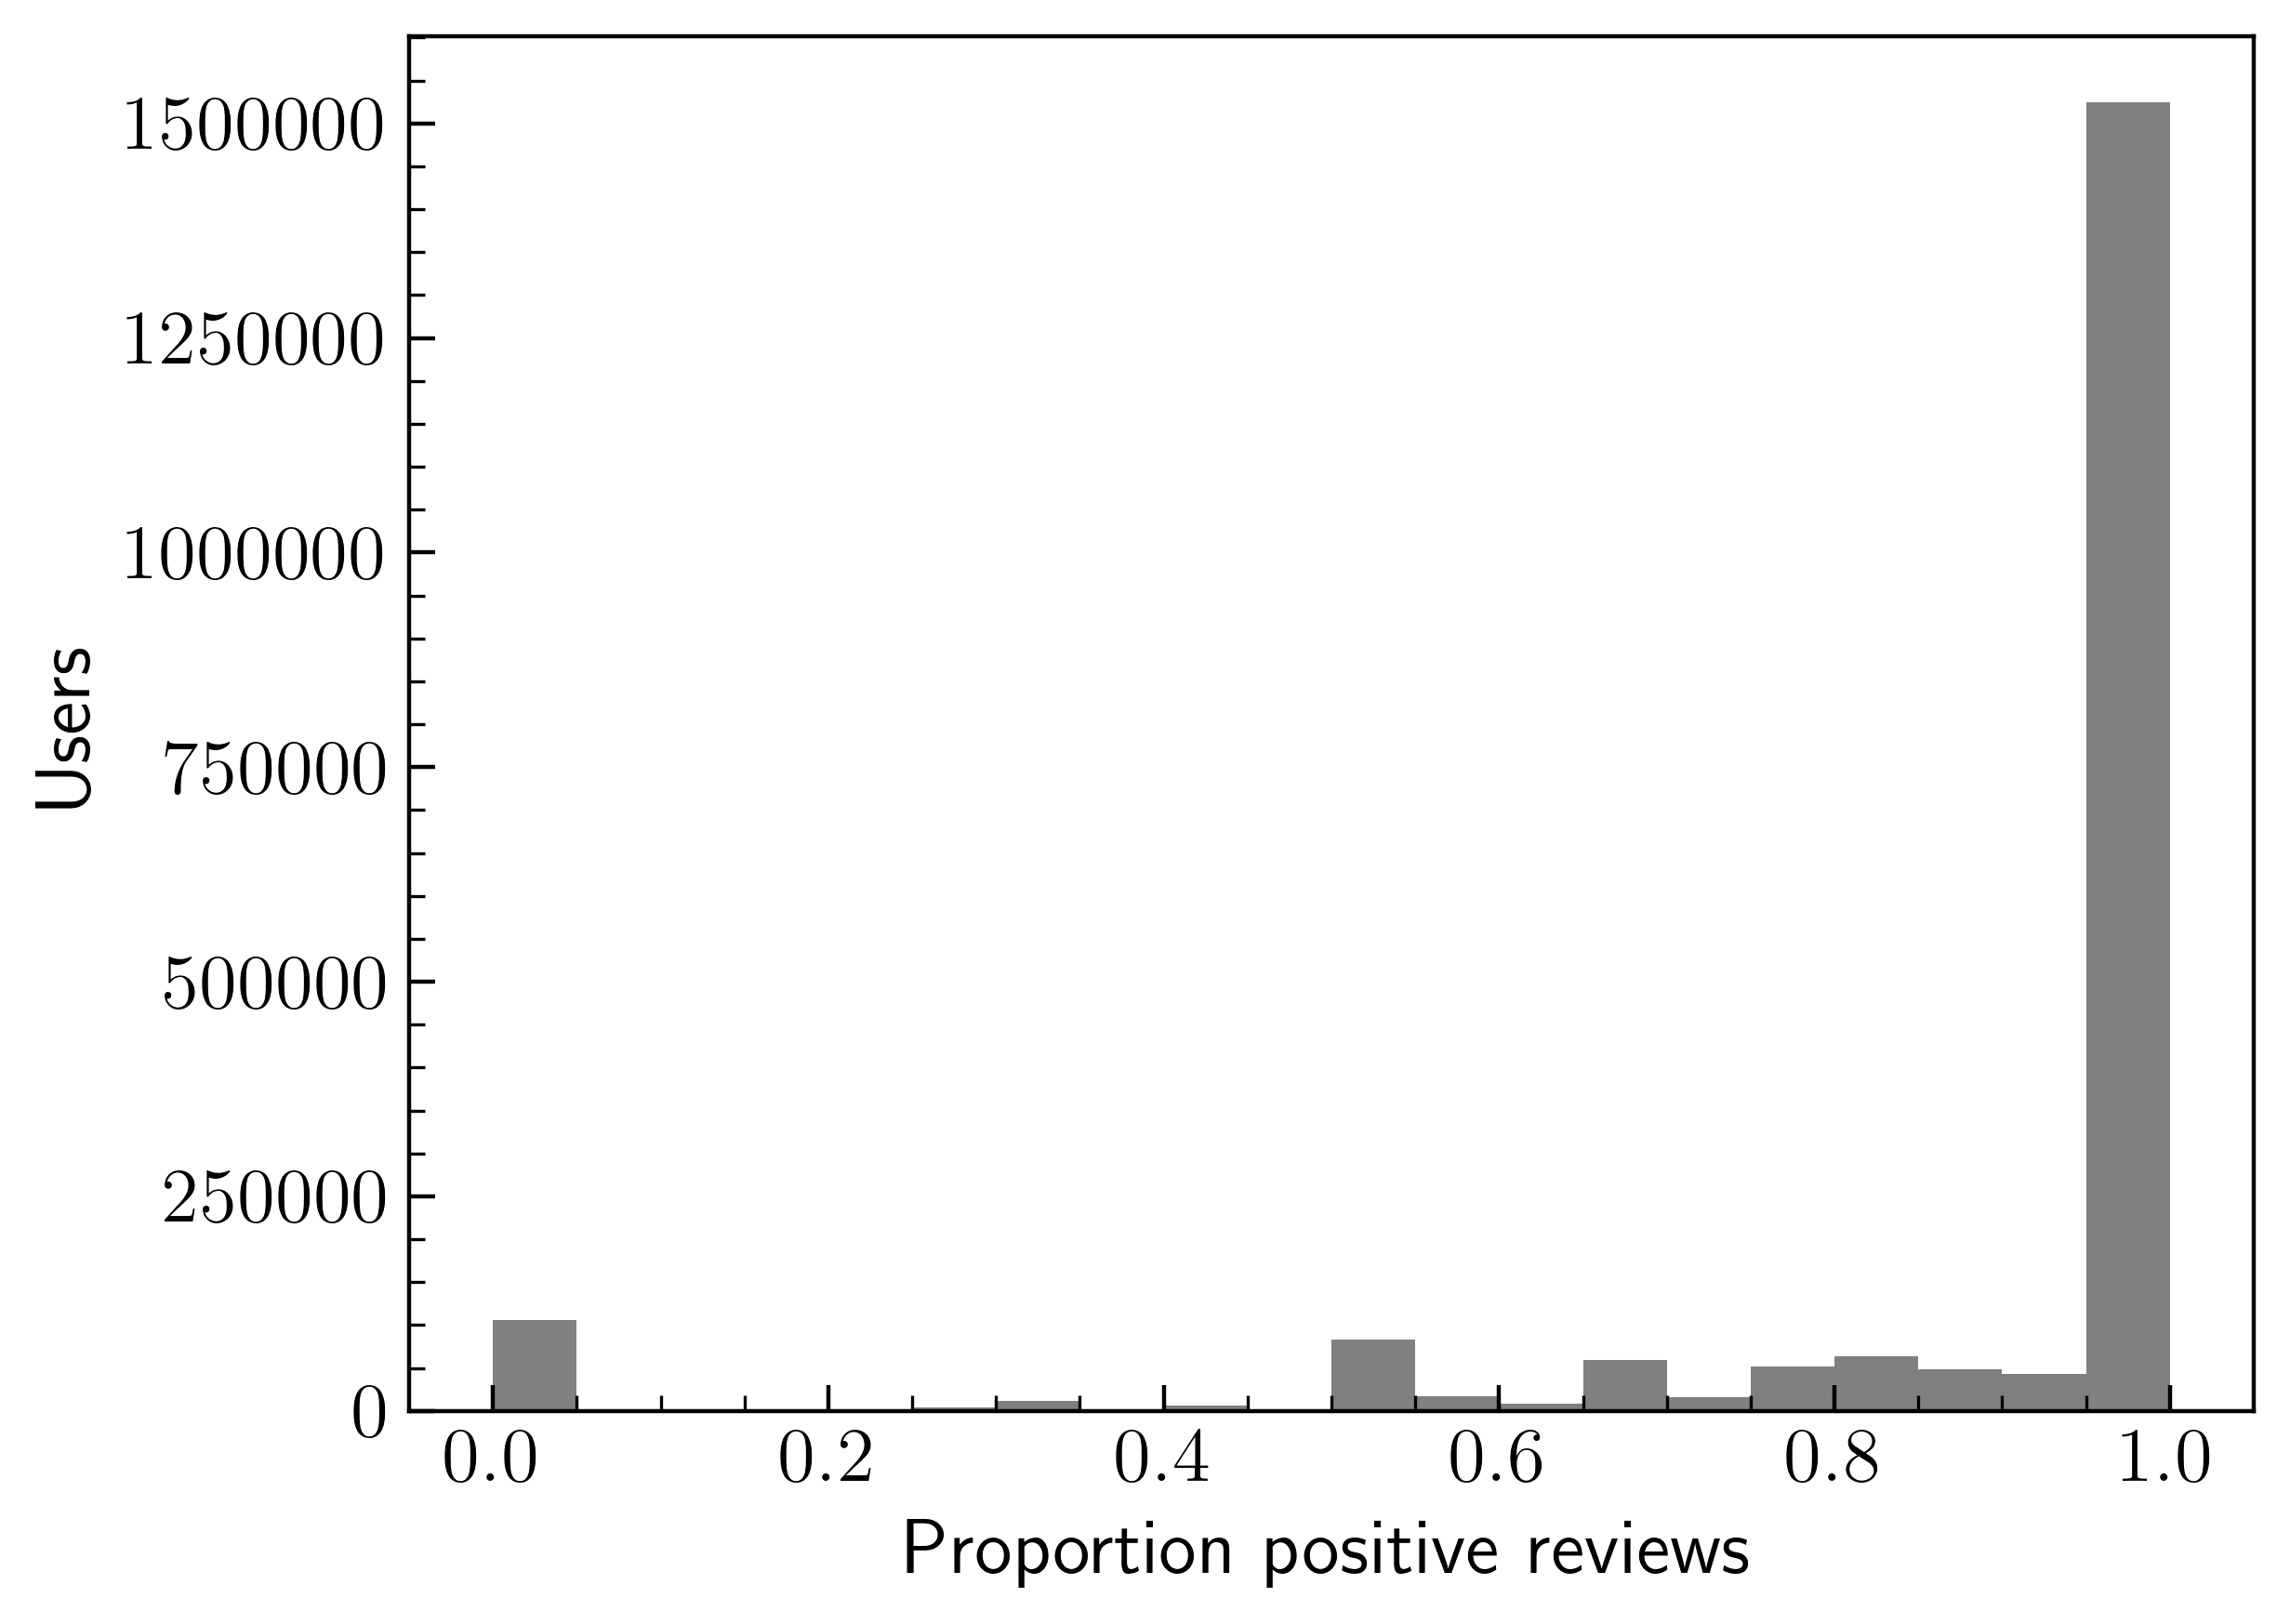
\includegraphics[width=\textwidth]{figures/03_dataset/06_hist_user_polarities_min1.png}
        \caption{All users.}
        \label{fig:Dataset_HistPolaritiesMin1}
    \end{subfigure}
    \hfill
    \begin{subfigure}[ht]{0.49\textwidth}
        \centering
        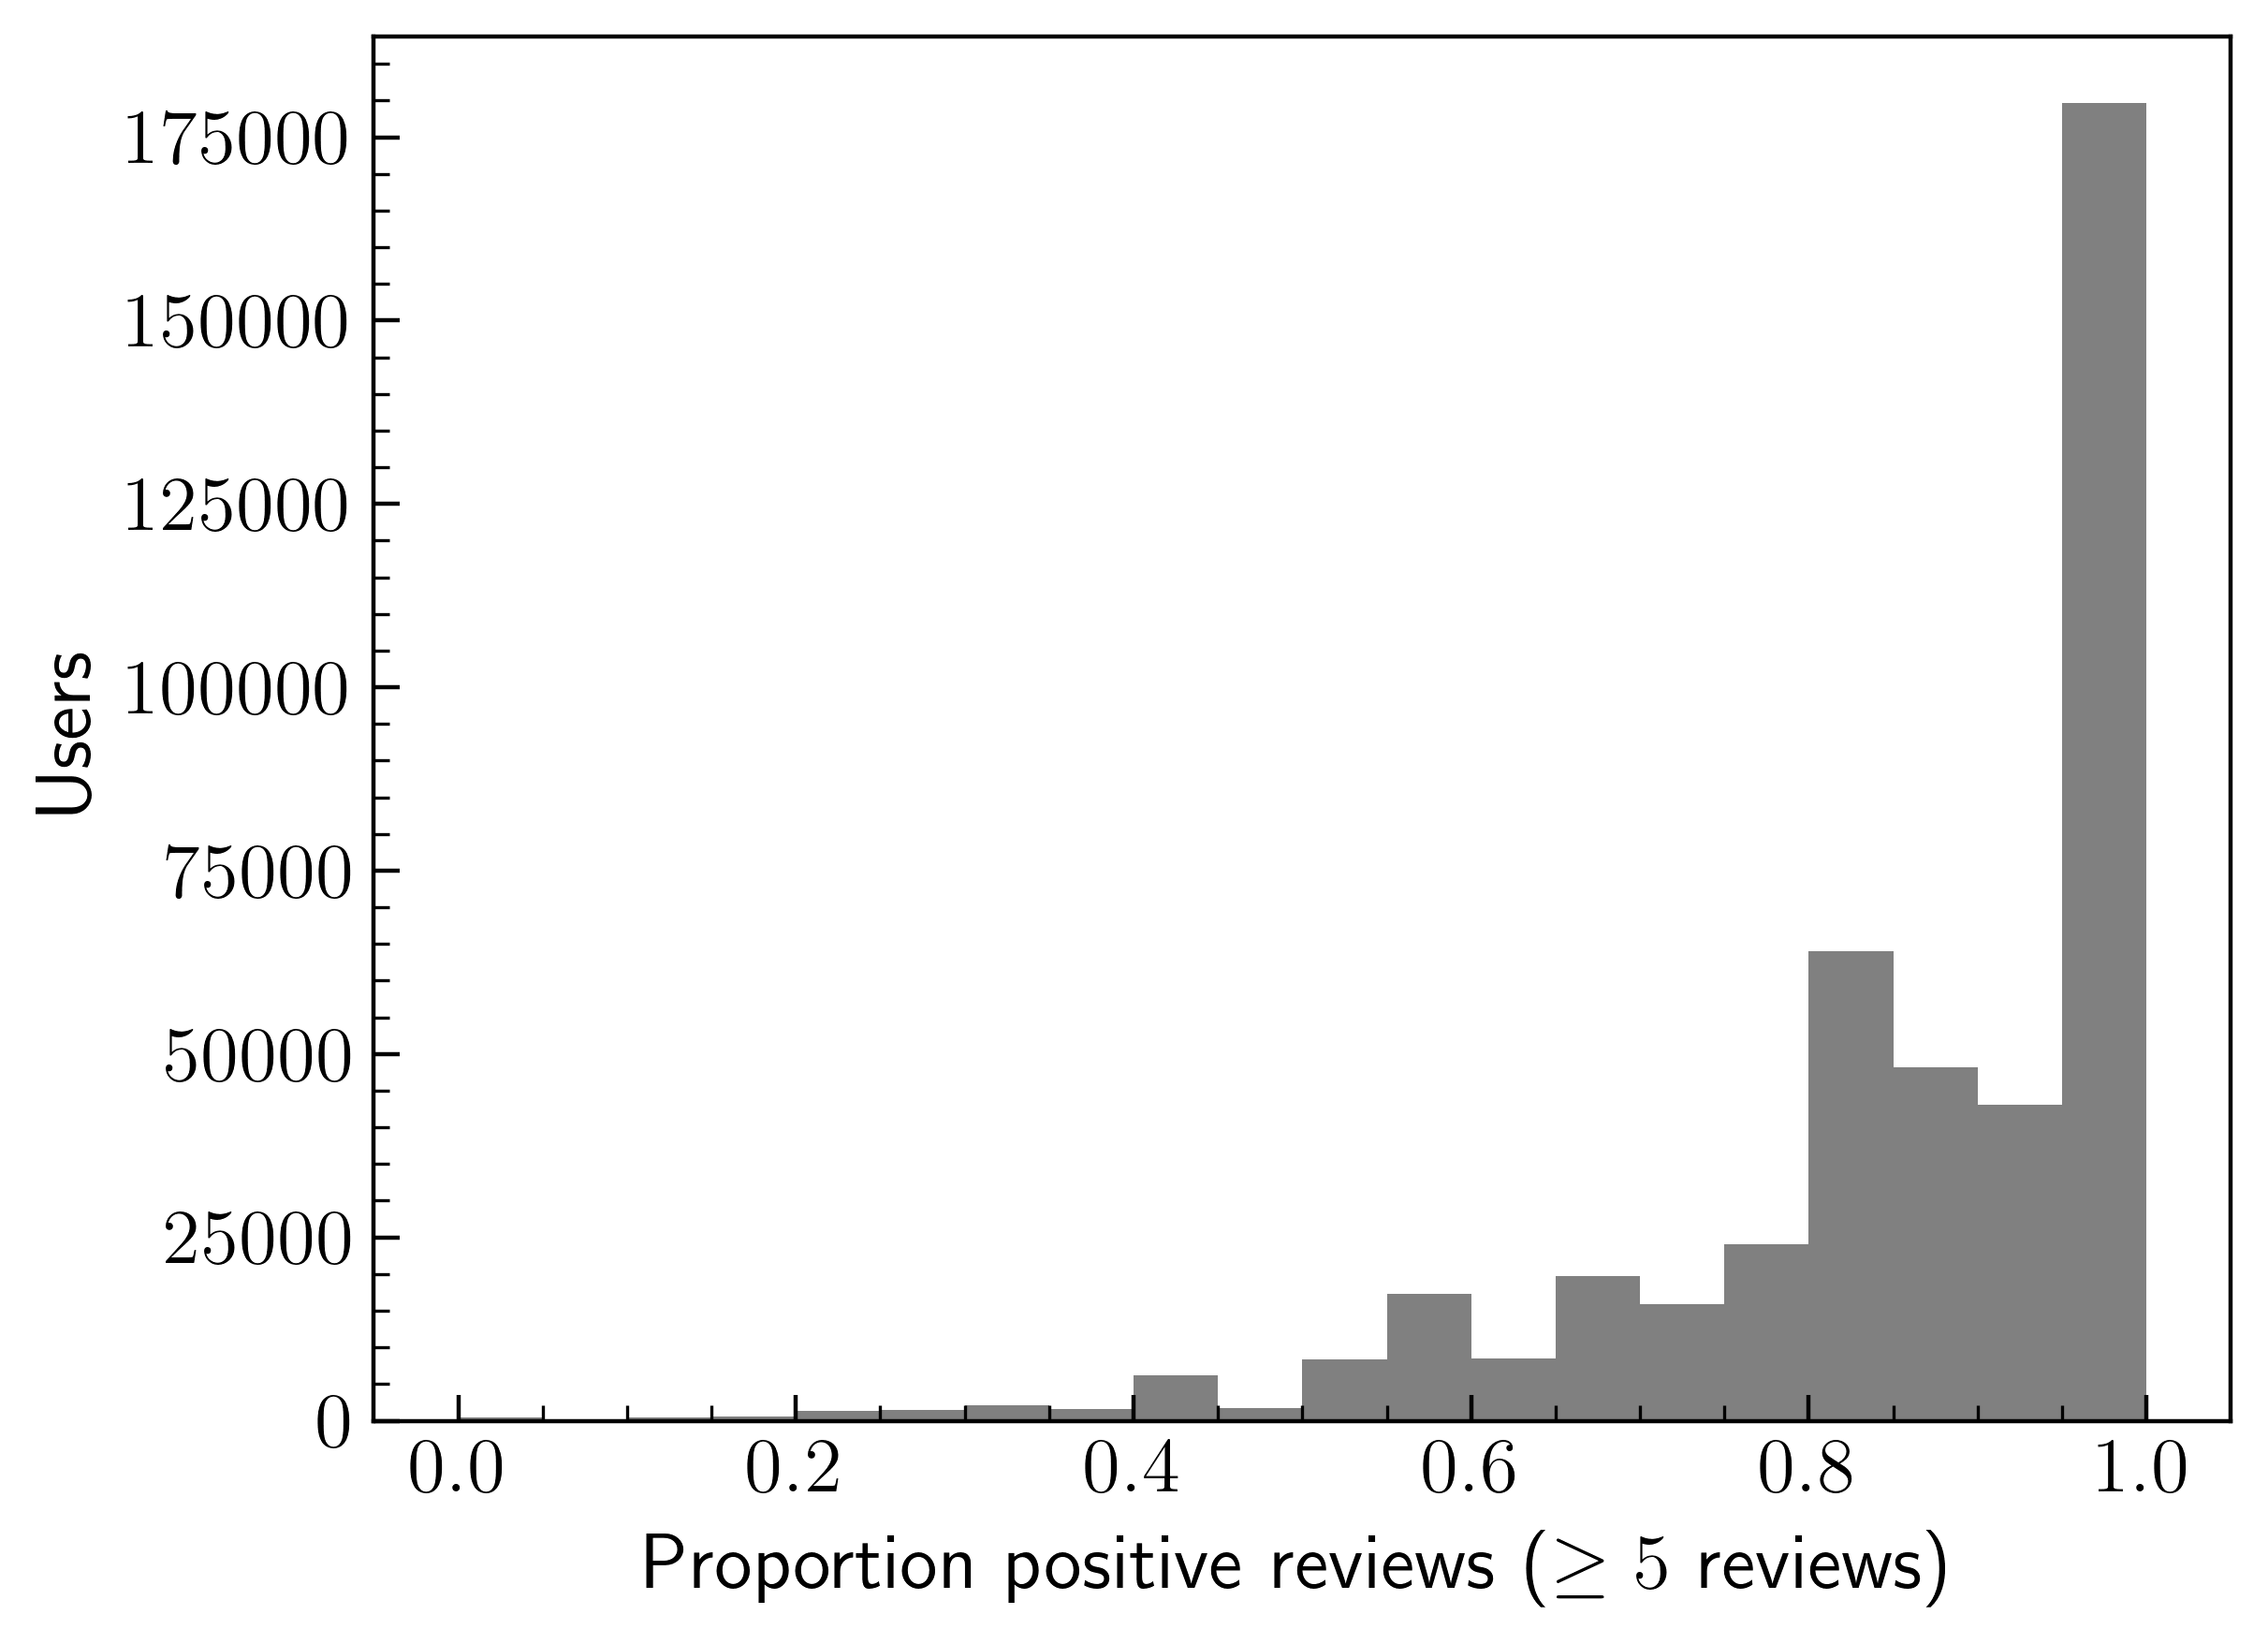
\includegraphics[width=\textwidth]{figures/03_dataset/07_hist_user_polarities_min5.png}
        \caption{Users with at least five reviews.}
        \label{fig:Dataset_HistPolaritiesMin5}
    \end{subfigure}
    \caption{Proportion of users' reviews that are positive.}
    \label{fig:Dataset_HistsPolarities}
\end{figure}

\subsection{Miscellaneous Features}

The distribution of some review features can be seen in Figure \ref{fig:Dataset_BarsCounts}. Across the dataset, 85\% of reviews are positive, 9.6\% are for an early access game and 14.4\% were updated by the author at some point.

\begin{figure}[ht]
    \centering
    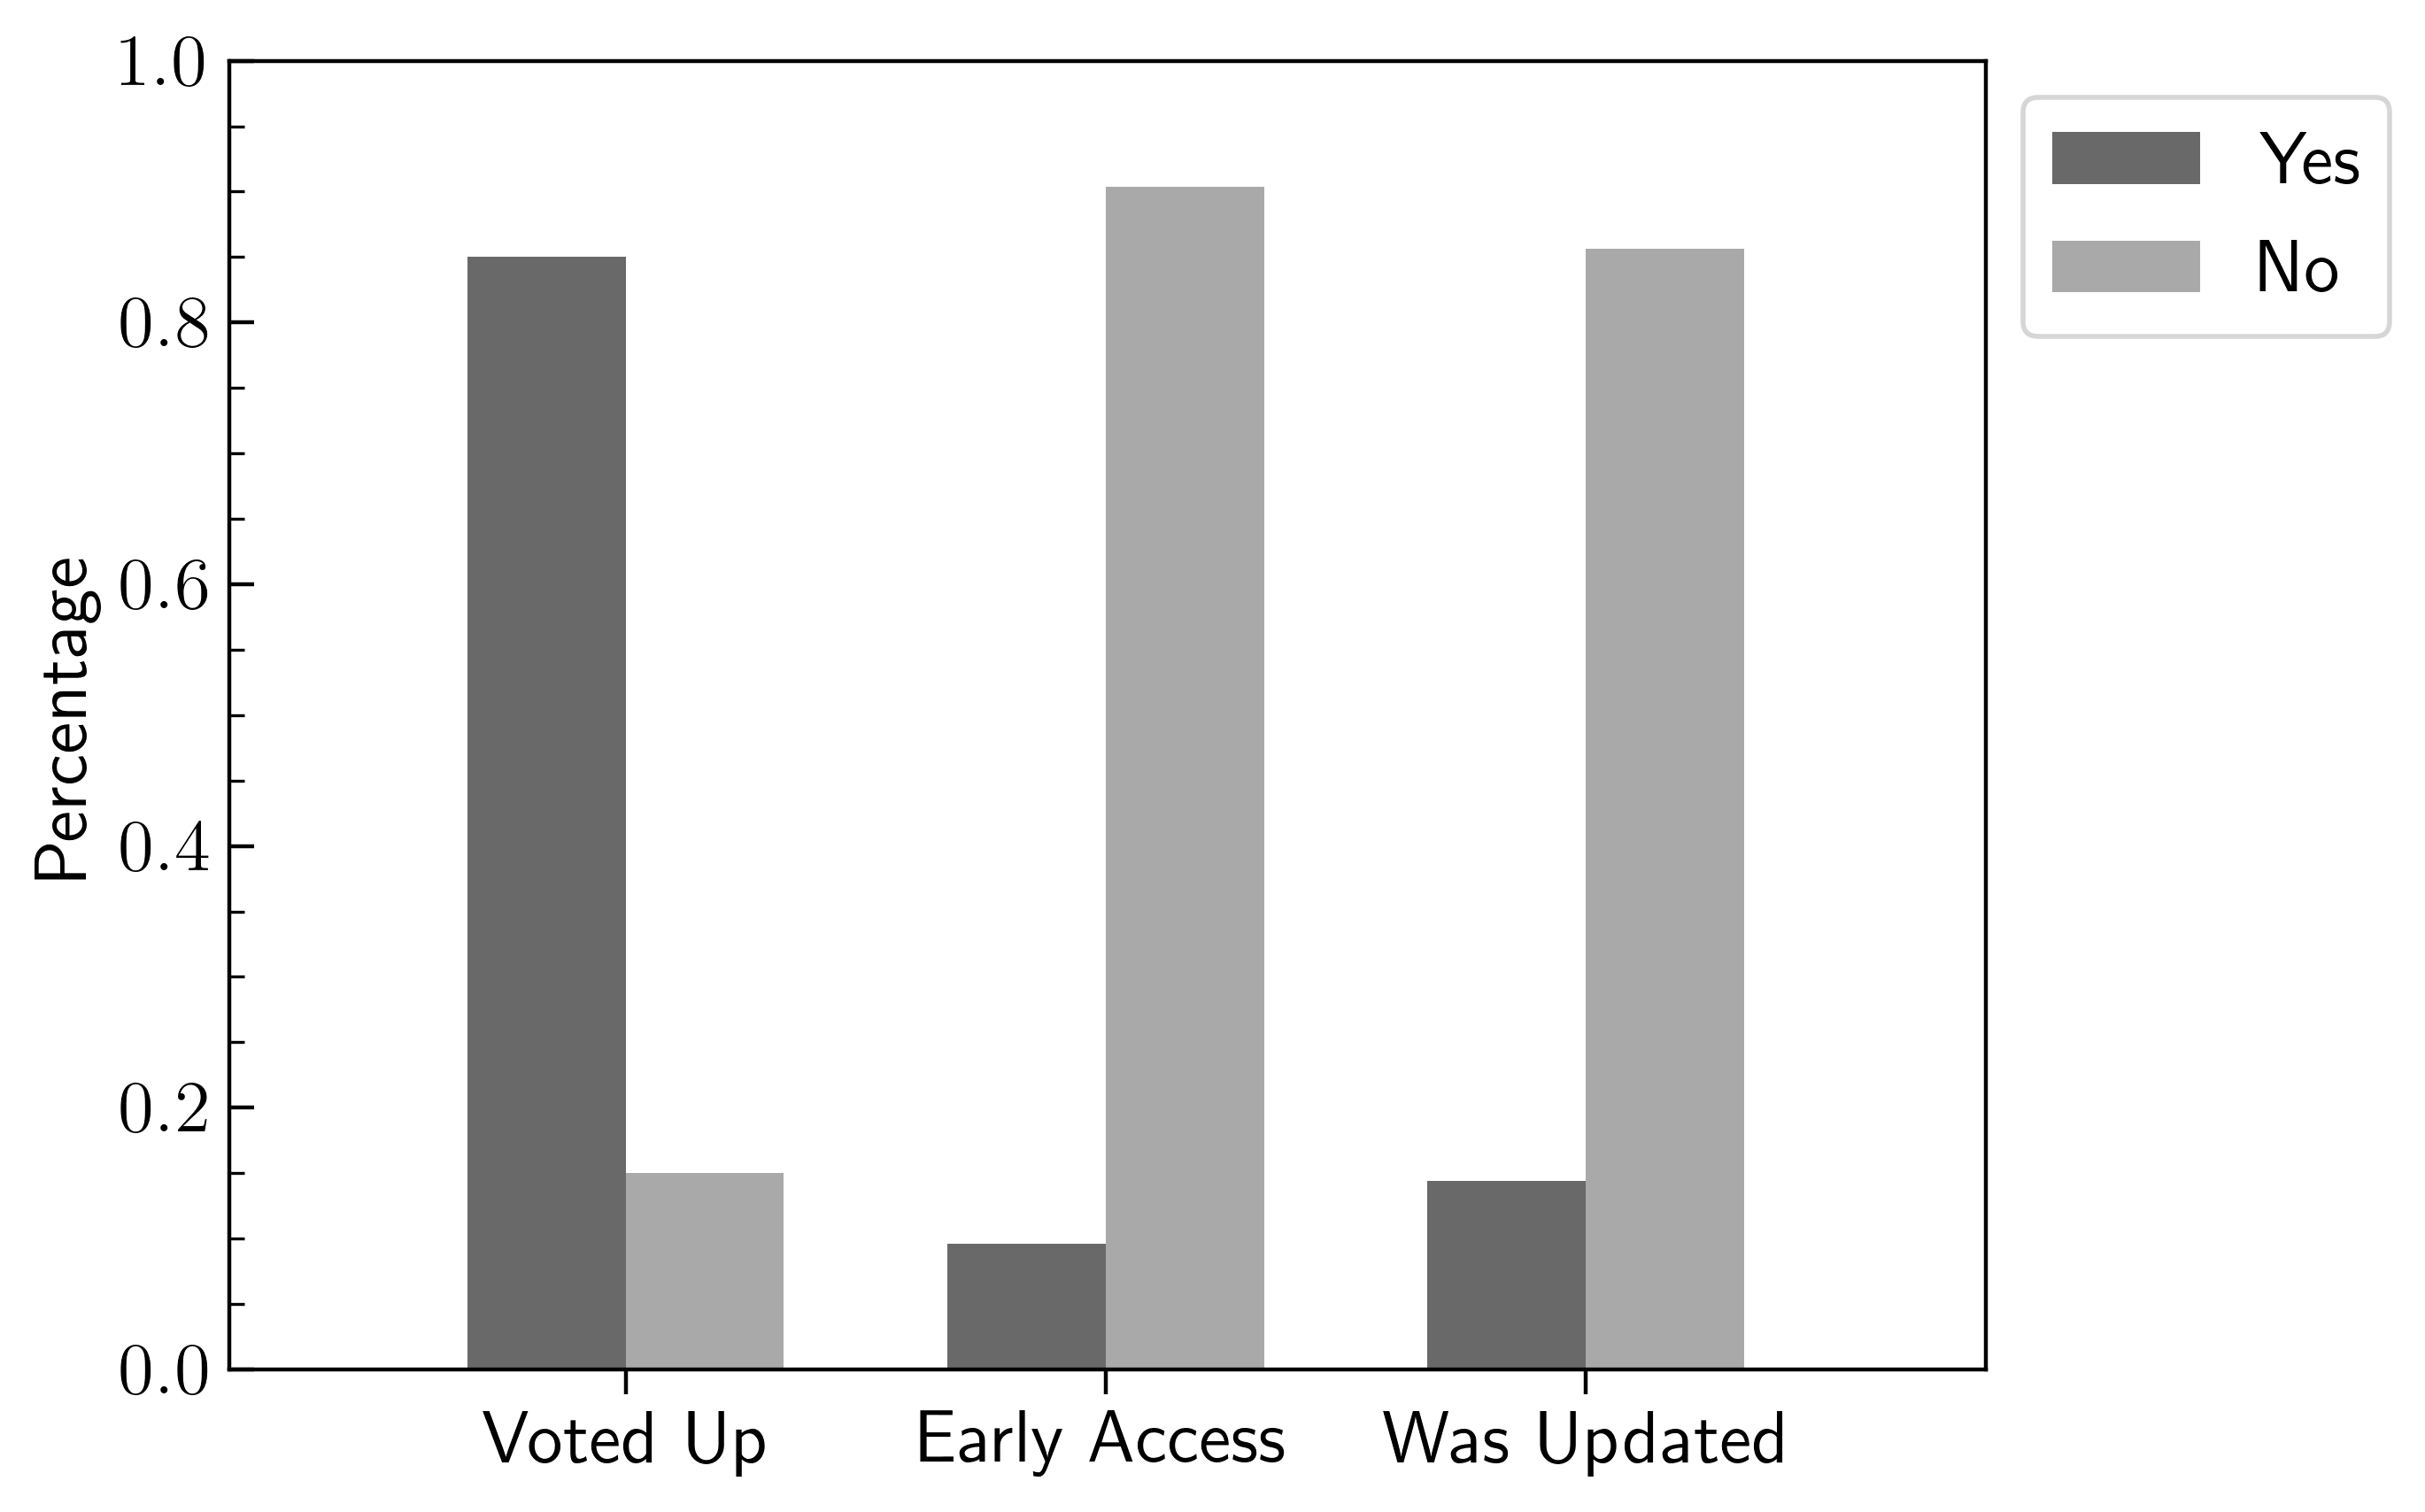
\includegraphics[scale=0.55]{figures/03_dataset/08_bars_counts.png}
    \caption{Percentage of reviews that were positive (voted up), early access and updated.}
    \label{fig:Dataset_BarsCounts}
\end{figure}

\subsection{Timestamps}

The years in which reviews were written can be seen in Figure \ref{fig:Dataset_BarsTimestamps}.

\begin{figure}[ht]
    \centering
    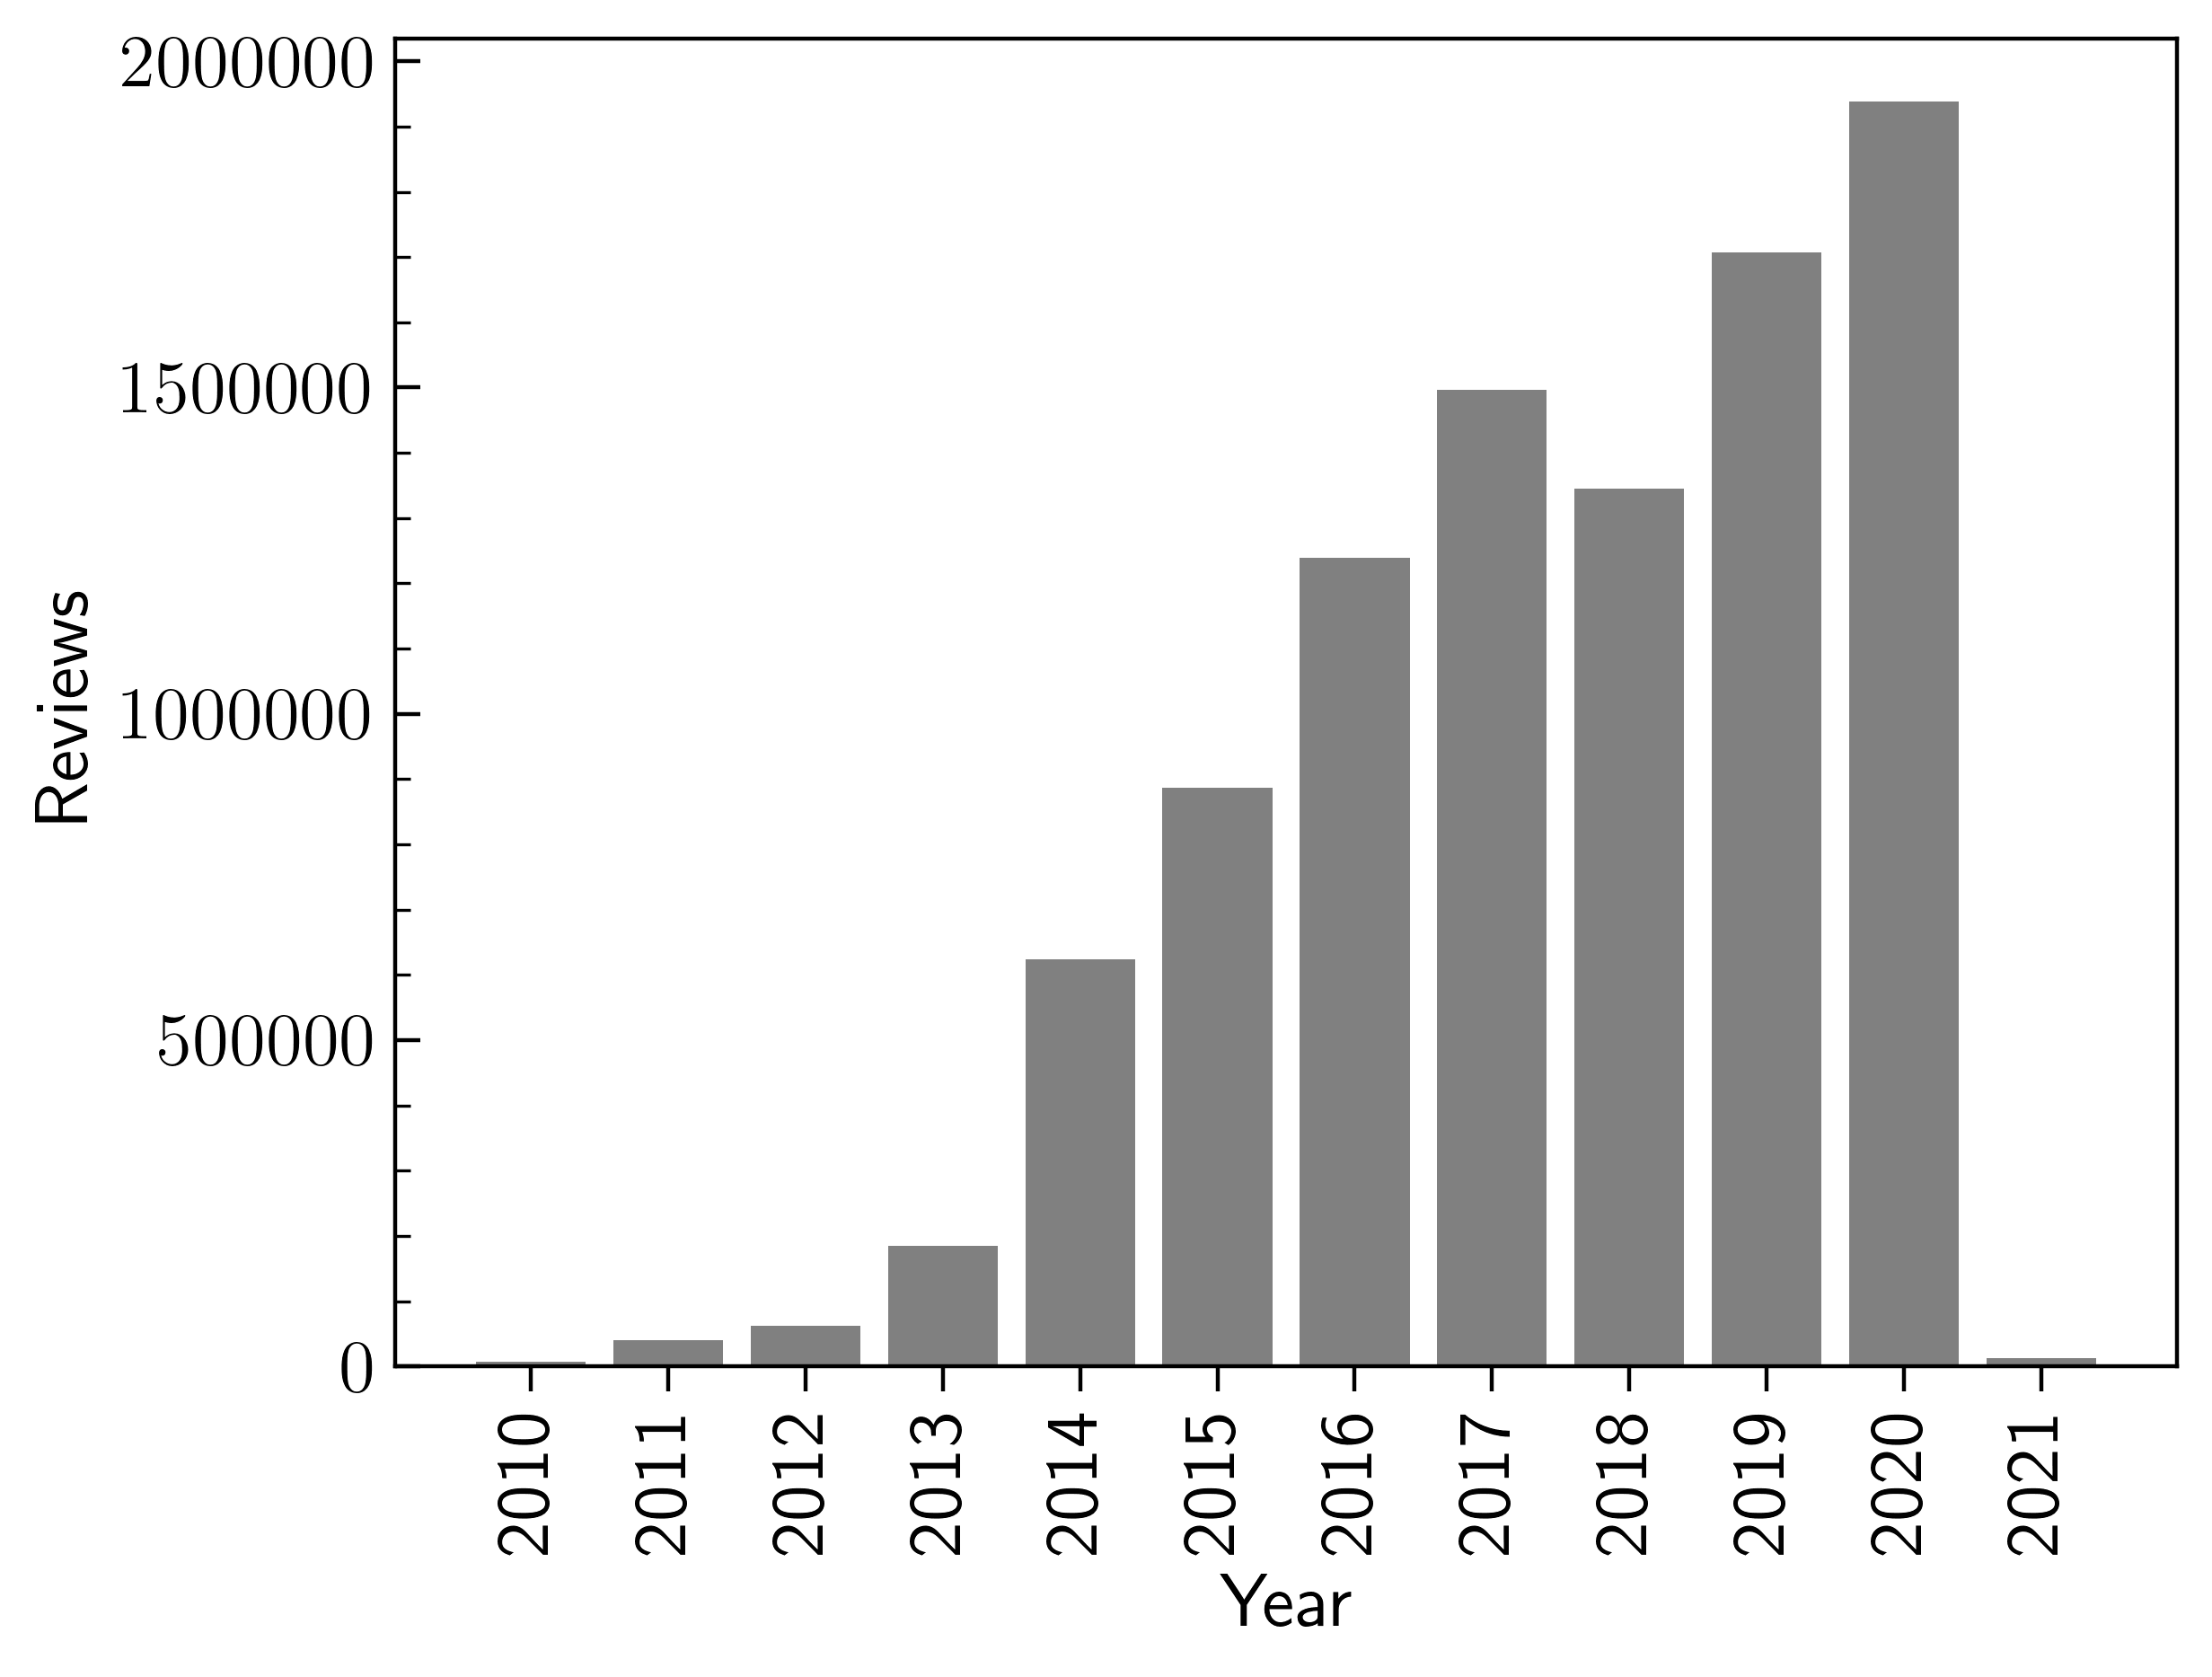
\includegraphics[scale=0.55]{figures/03_dataset/09_bars_review_dates.png}
    \caption{Years in which reviews were written.}
    \label{fig:Dataset_BarsTimestamps}
\end{figure}

\subsection{Playtime}

The amount of hours that users played the games they reviewed (in total) can be seen in Figure \ref{fig:Dataset_HistPlaytimes}. Reviews where the user played the game for over 152.4 hours, 16.4\% of all reviews, have been excluded from the histogram. The mean amount of hours users played the games they reviewed is 159.1 (\textit{SD} = 540.6) and the median is 12.2. 25\% of users played the game they reviewed for 2.9 hours or less and 75\% of users played the game they reviewed for 62.7 hours or less.

\begin{figure}[ht]
    \centering
    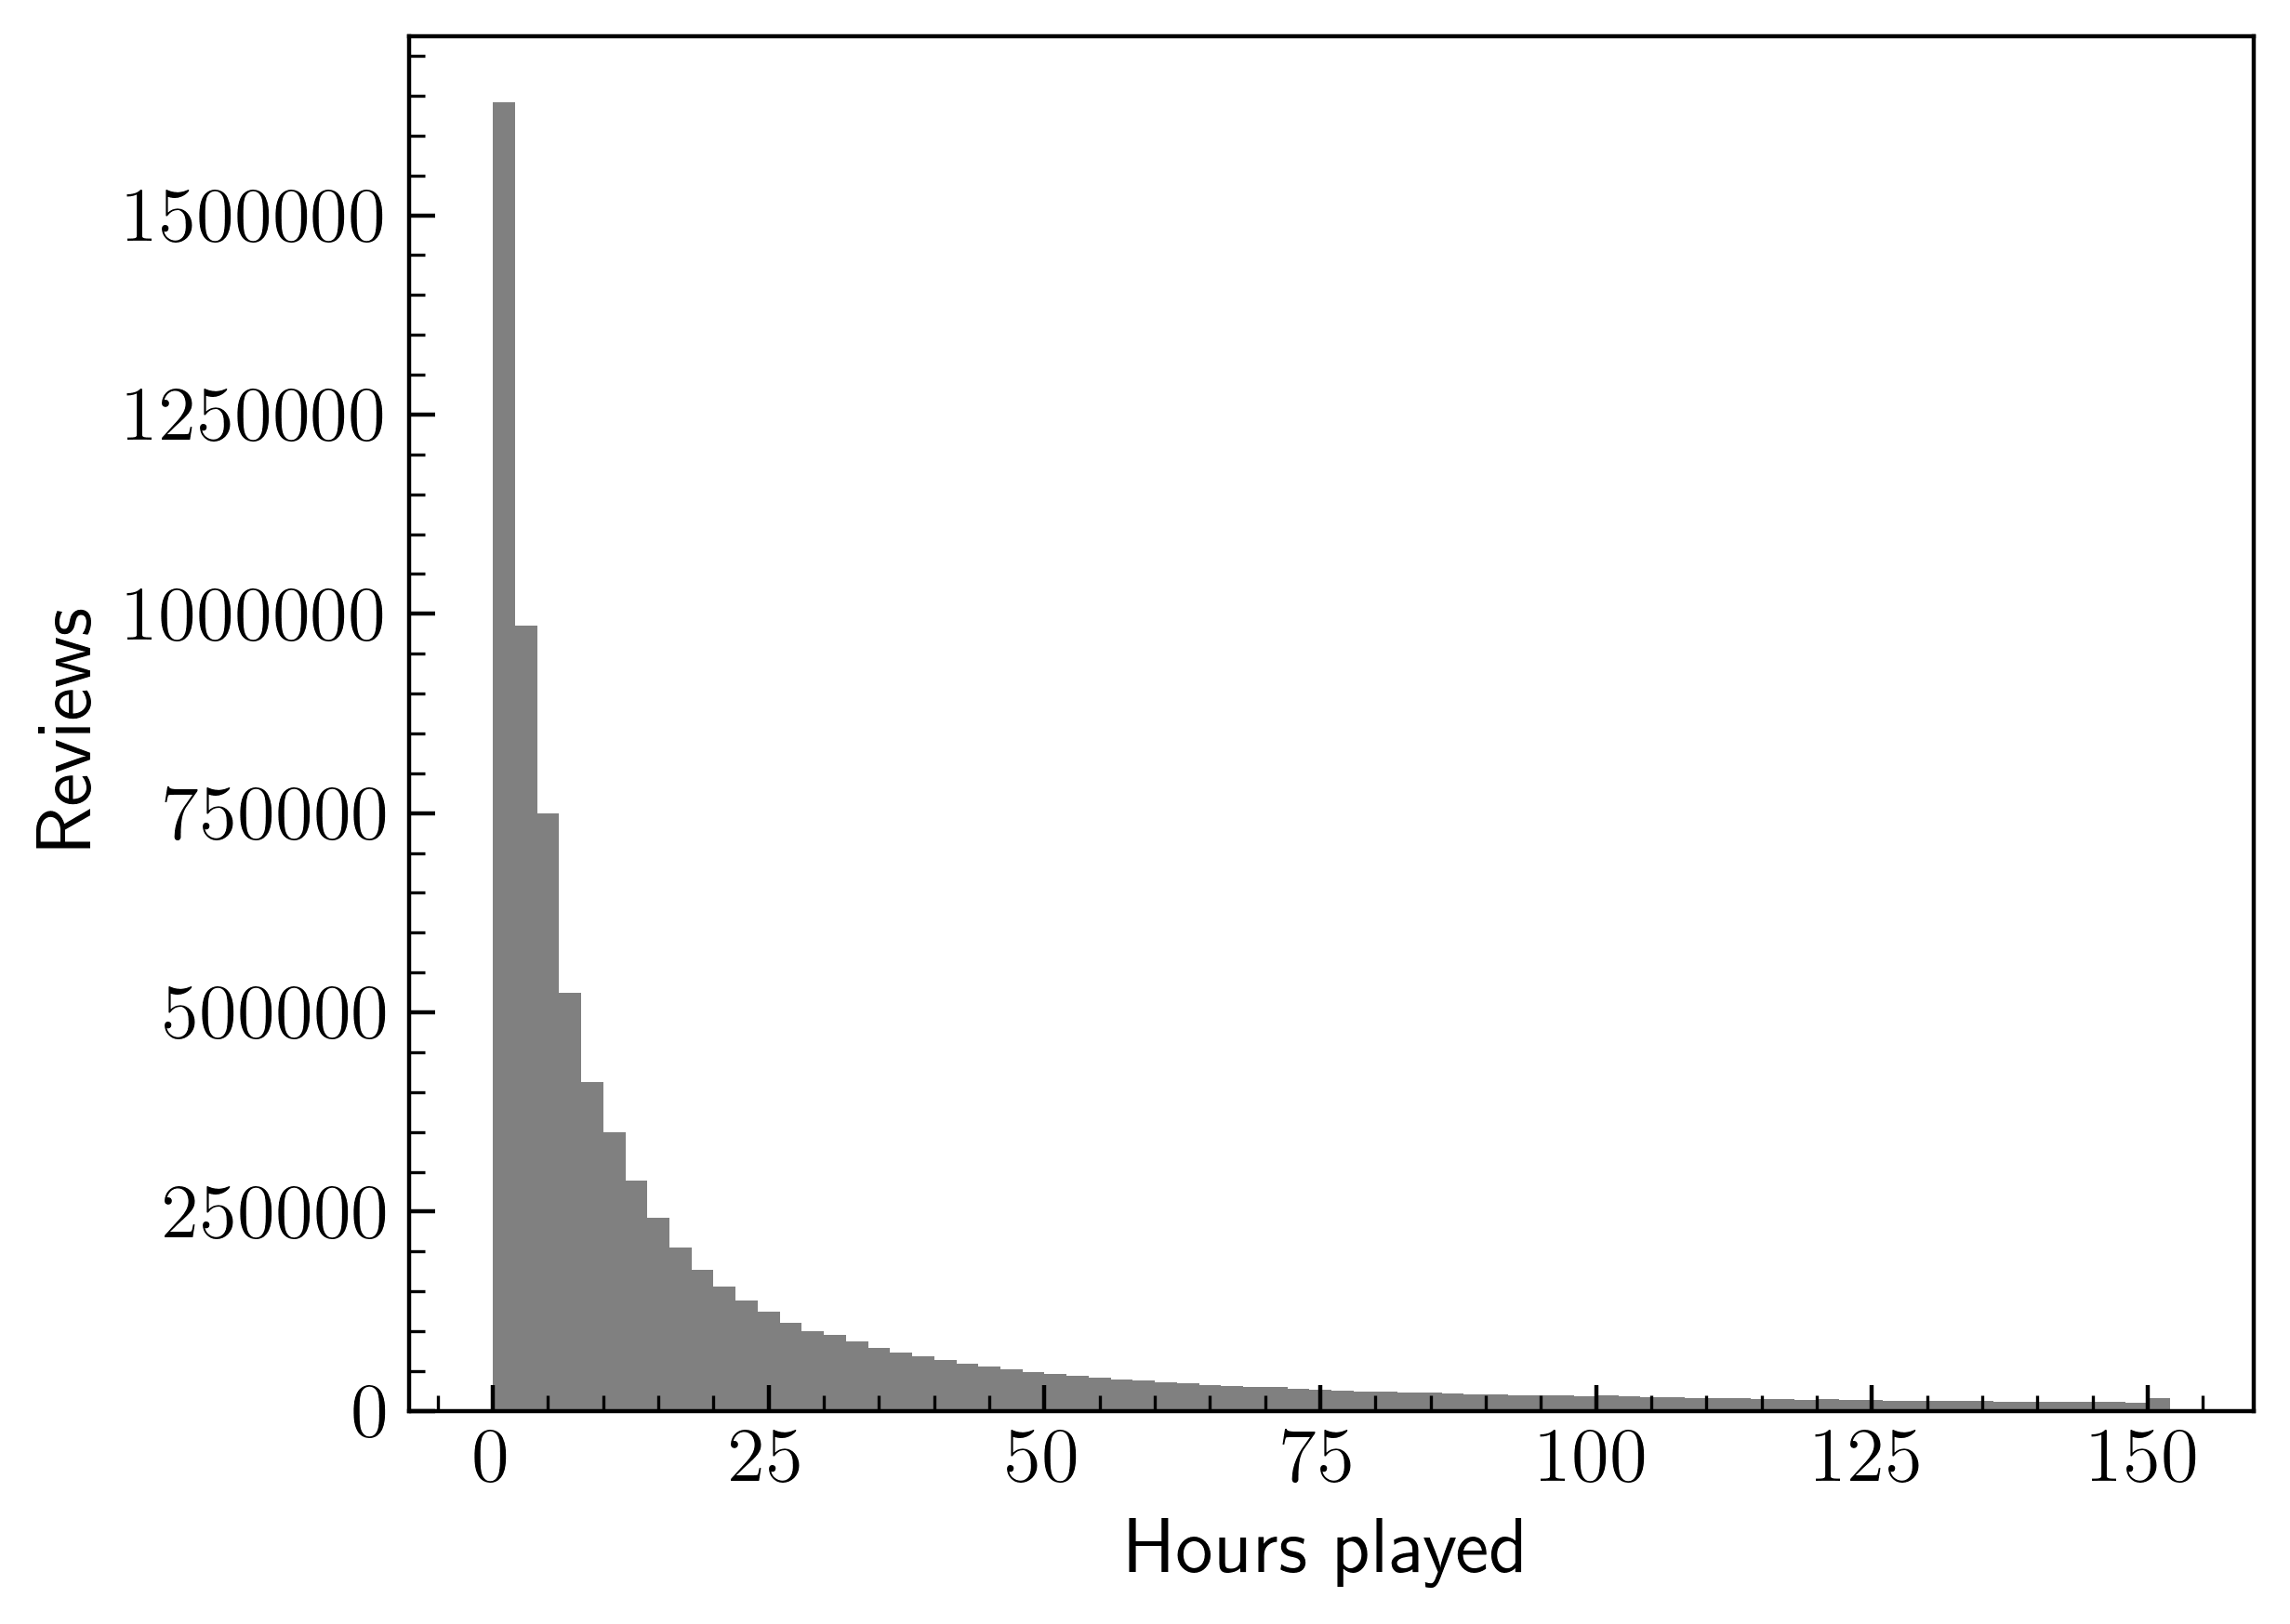
\includegraphics[scale=0.55]{figures/03_dataset/10_hist_review_playtimes.png}
    \caption{Number of hours that reviewed games were played (in total).}
    \label{fig:Dataset_HistPlaytimes}
\end{figure}

\subsection{Votes}

The number of votes up that reviews received can be seen in Figure \ref{fig:Dataset_HistVotes}. Reviews with more than 17 votes, 4.5\% of all reviews, have been excluded from the histogram. The mean number of votes reviews received is 4.3 (\textit{SD} = 22.9) and the median is 0. A majority of reviews didn't receive a single vote and 75\% of reviews received 2 votes or fewer.

\begin{figure}[ht]
    \centering
    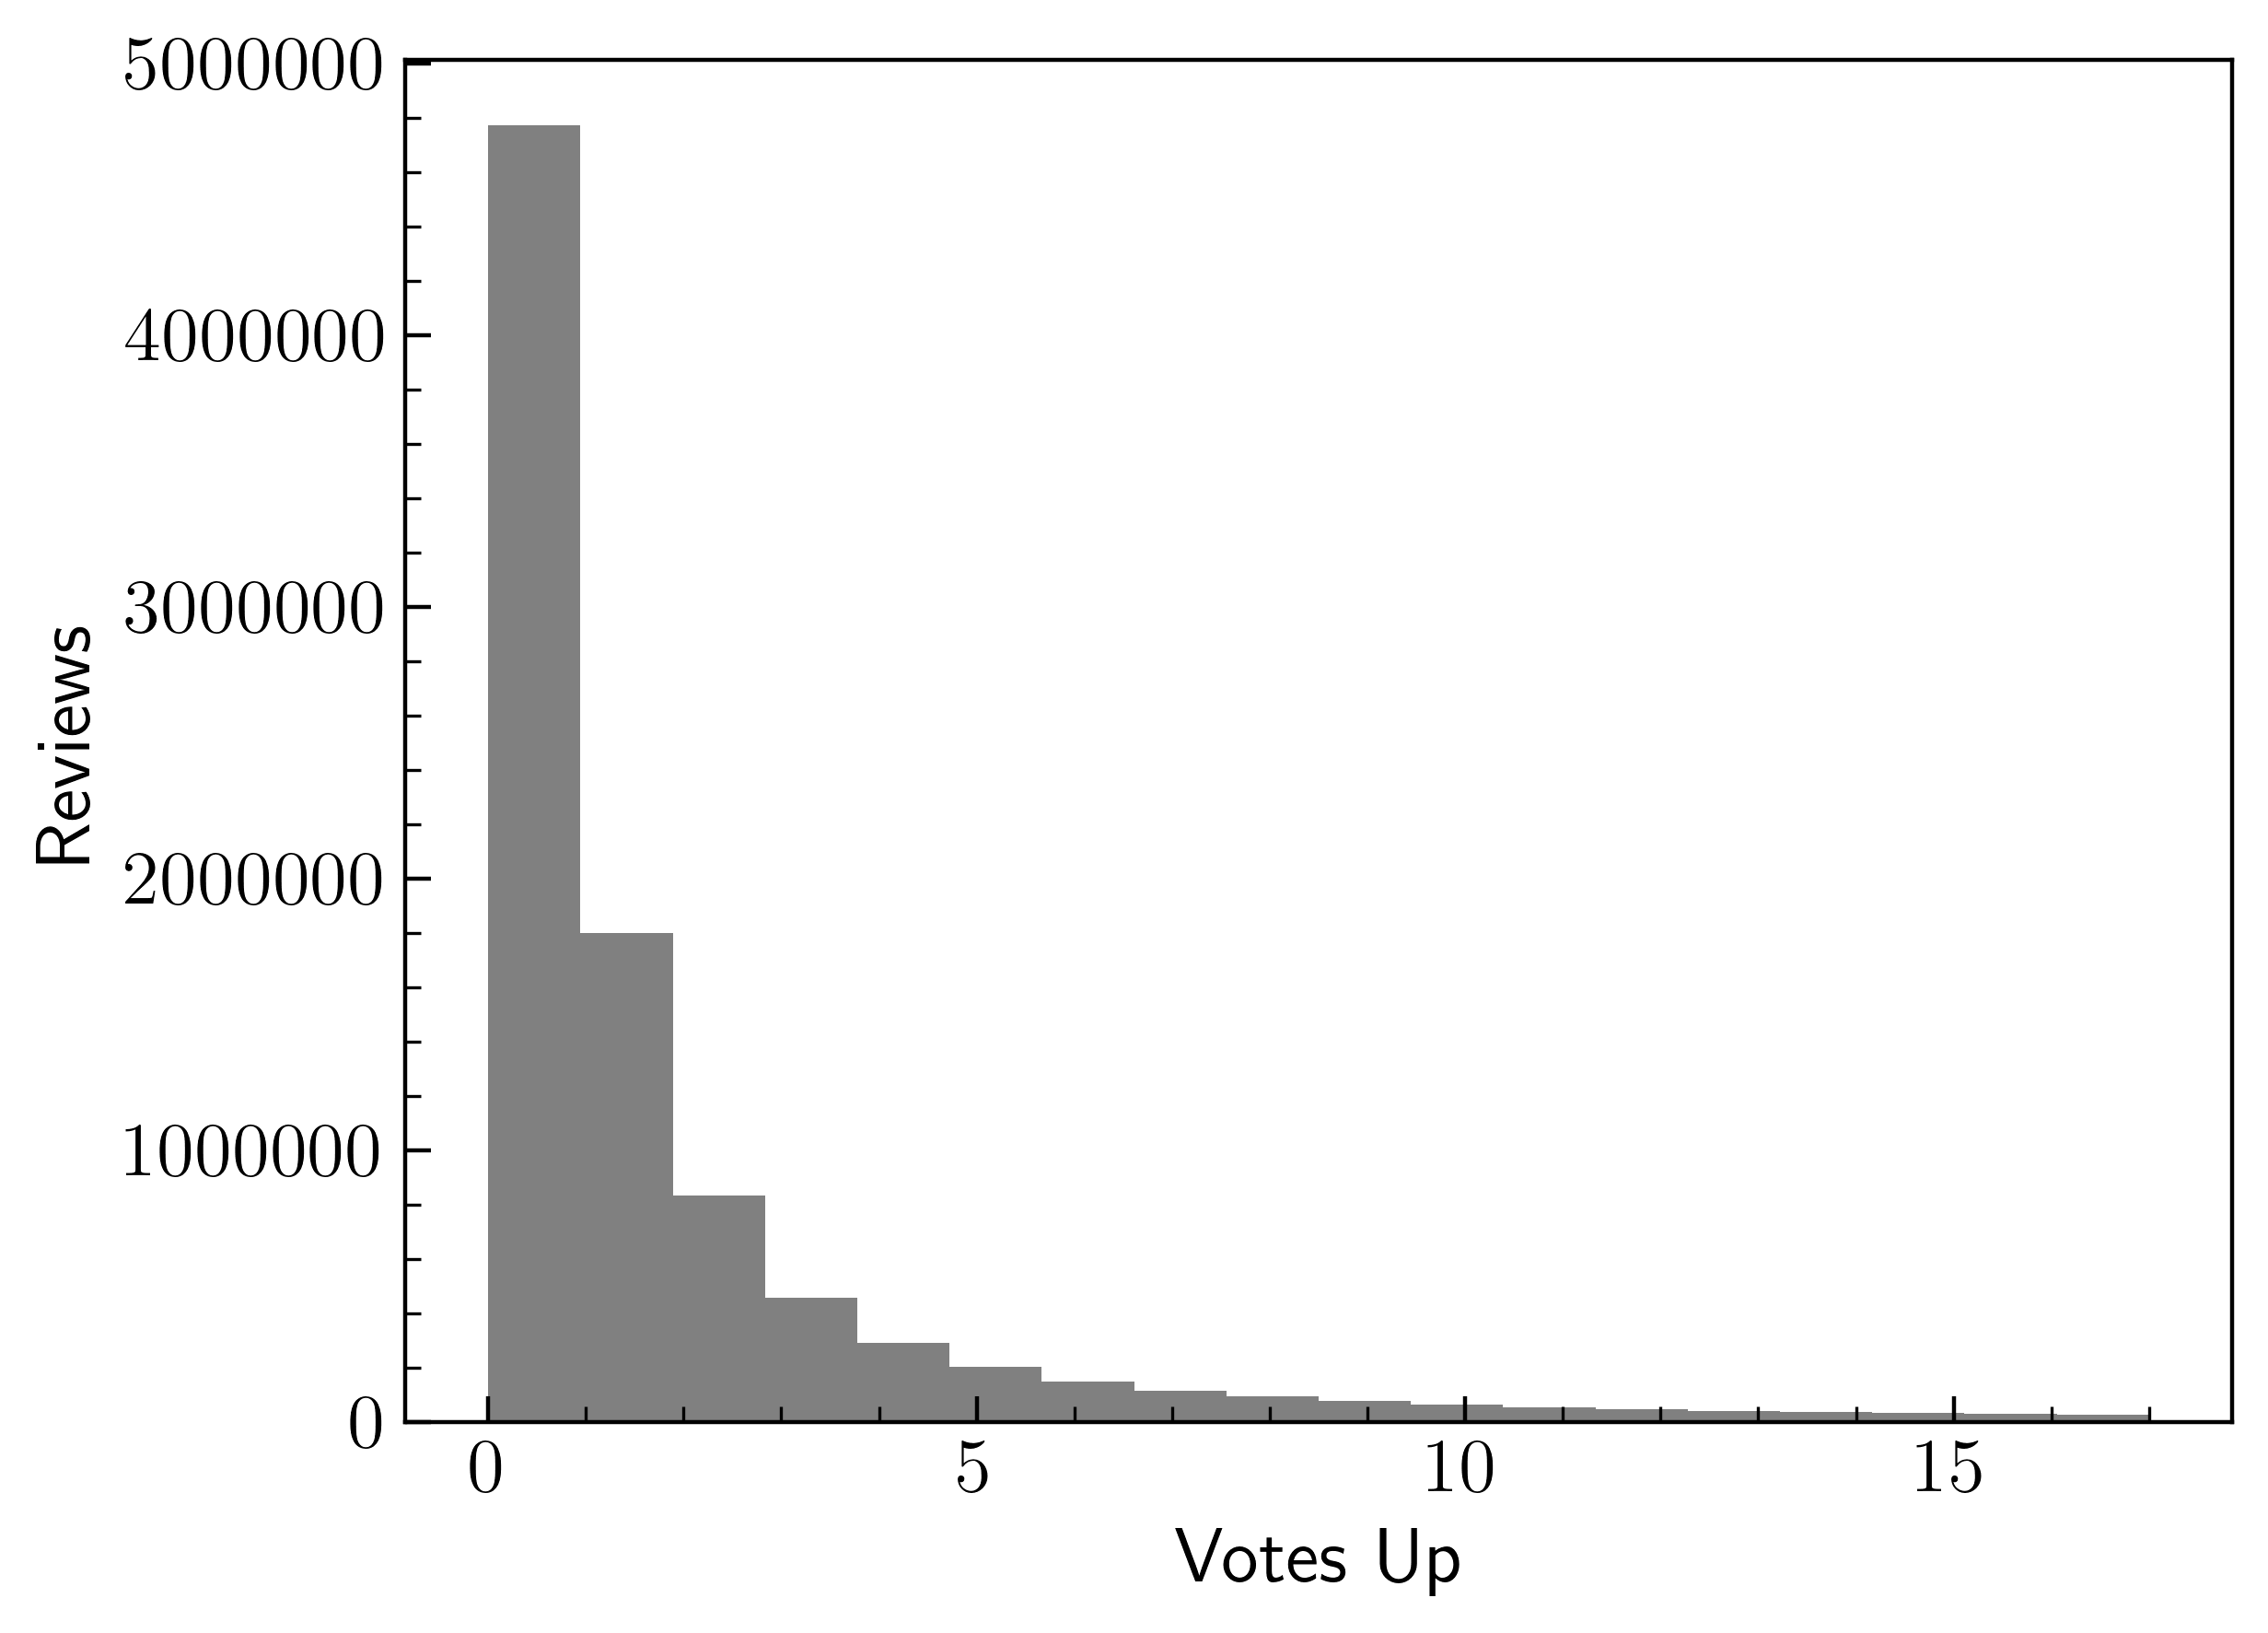
\includegraphics[scale=0.55]{figures/03_dataset/11_hist_review_votes.png}
    \caption{Number of votes up that reviews received.}
    \label{fig:Dataset_HistVotes}
\end{figure}

\section{Review Texts} \label{sec:Dataset_ReviewTexts}

The language each review was written in and the number of words each review contained was determined for nearly 70\% of all reviews in the dataset using the spaCy library in Python \cite{spacy}. Language detection is implemented using a Python port \cite{PyPi_LangDetect} of Google's language-detection library \cite{Nakatani2010_LangDetect} which supports over 50 languages.

\subsection{Languages}

The proportion of languages each review was written in can be seen in Figure \ref{fig:Dataset_BarsLangs}. Languages that less than 1\% of reviews are written in are excluded. Language proportions are shown for all reviews and for reviews with at least five words. When all reviews are considered the language detection algorithm fails to identify the language in approximately 3\% of reviews. When reviews with at least five words are considered this failure to identify the language occurs much less frequently and the proportion of reviews written in English increases to almost 50\%.

\begin{figure}[ht]
    \centering
    \begin{subfigure}[ht]{0.49\textwidth}
        \centering
        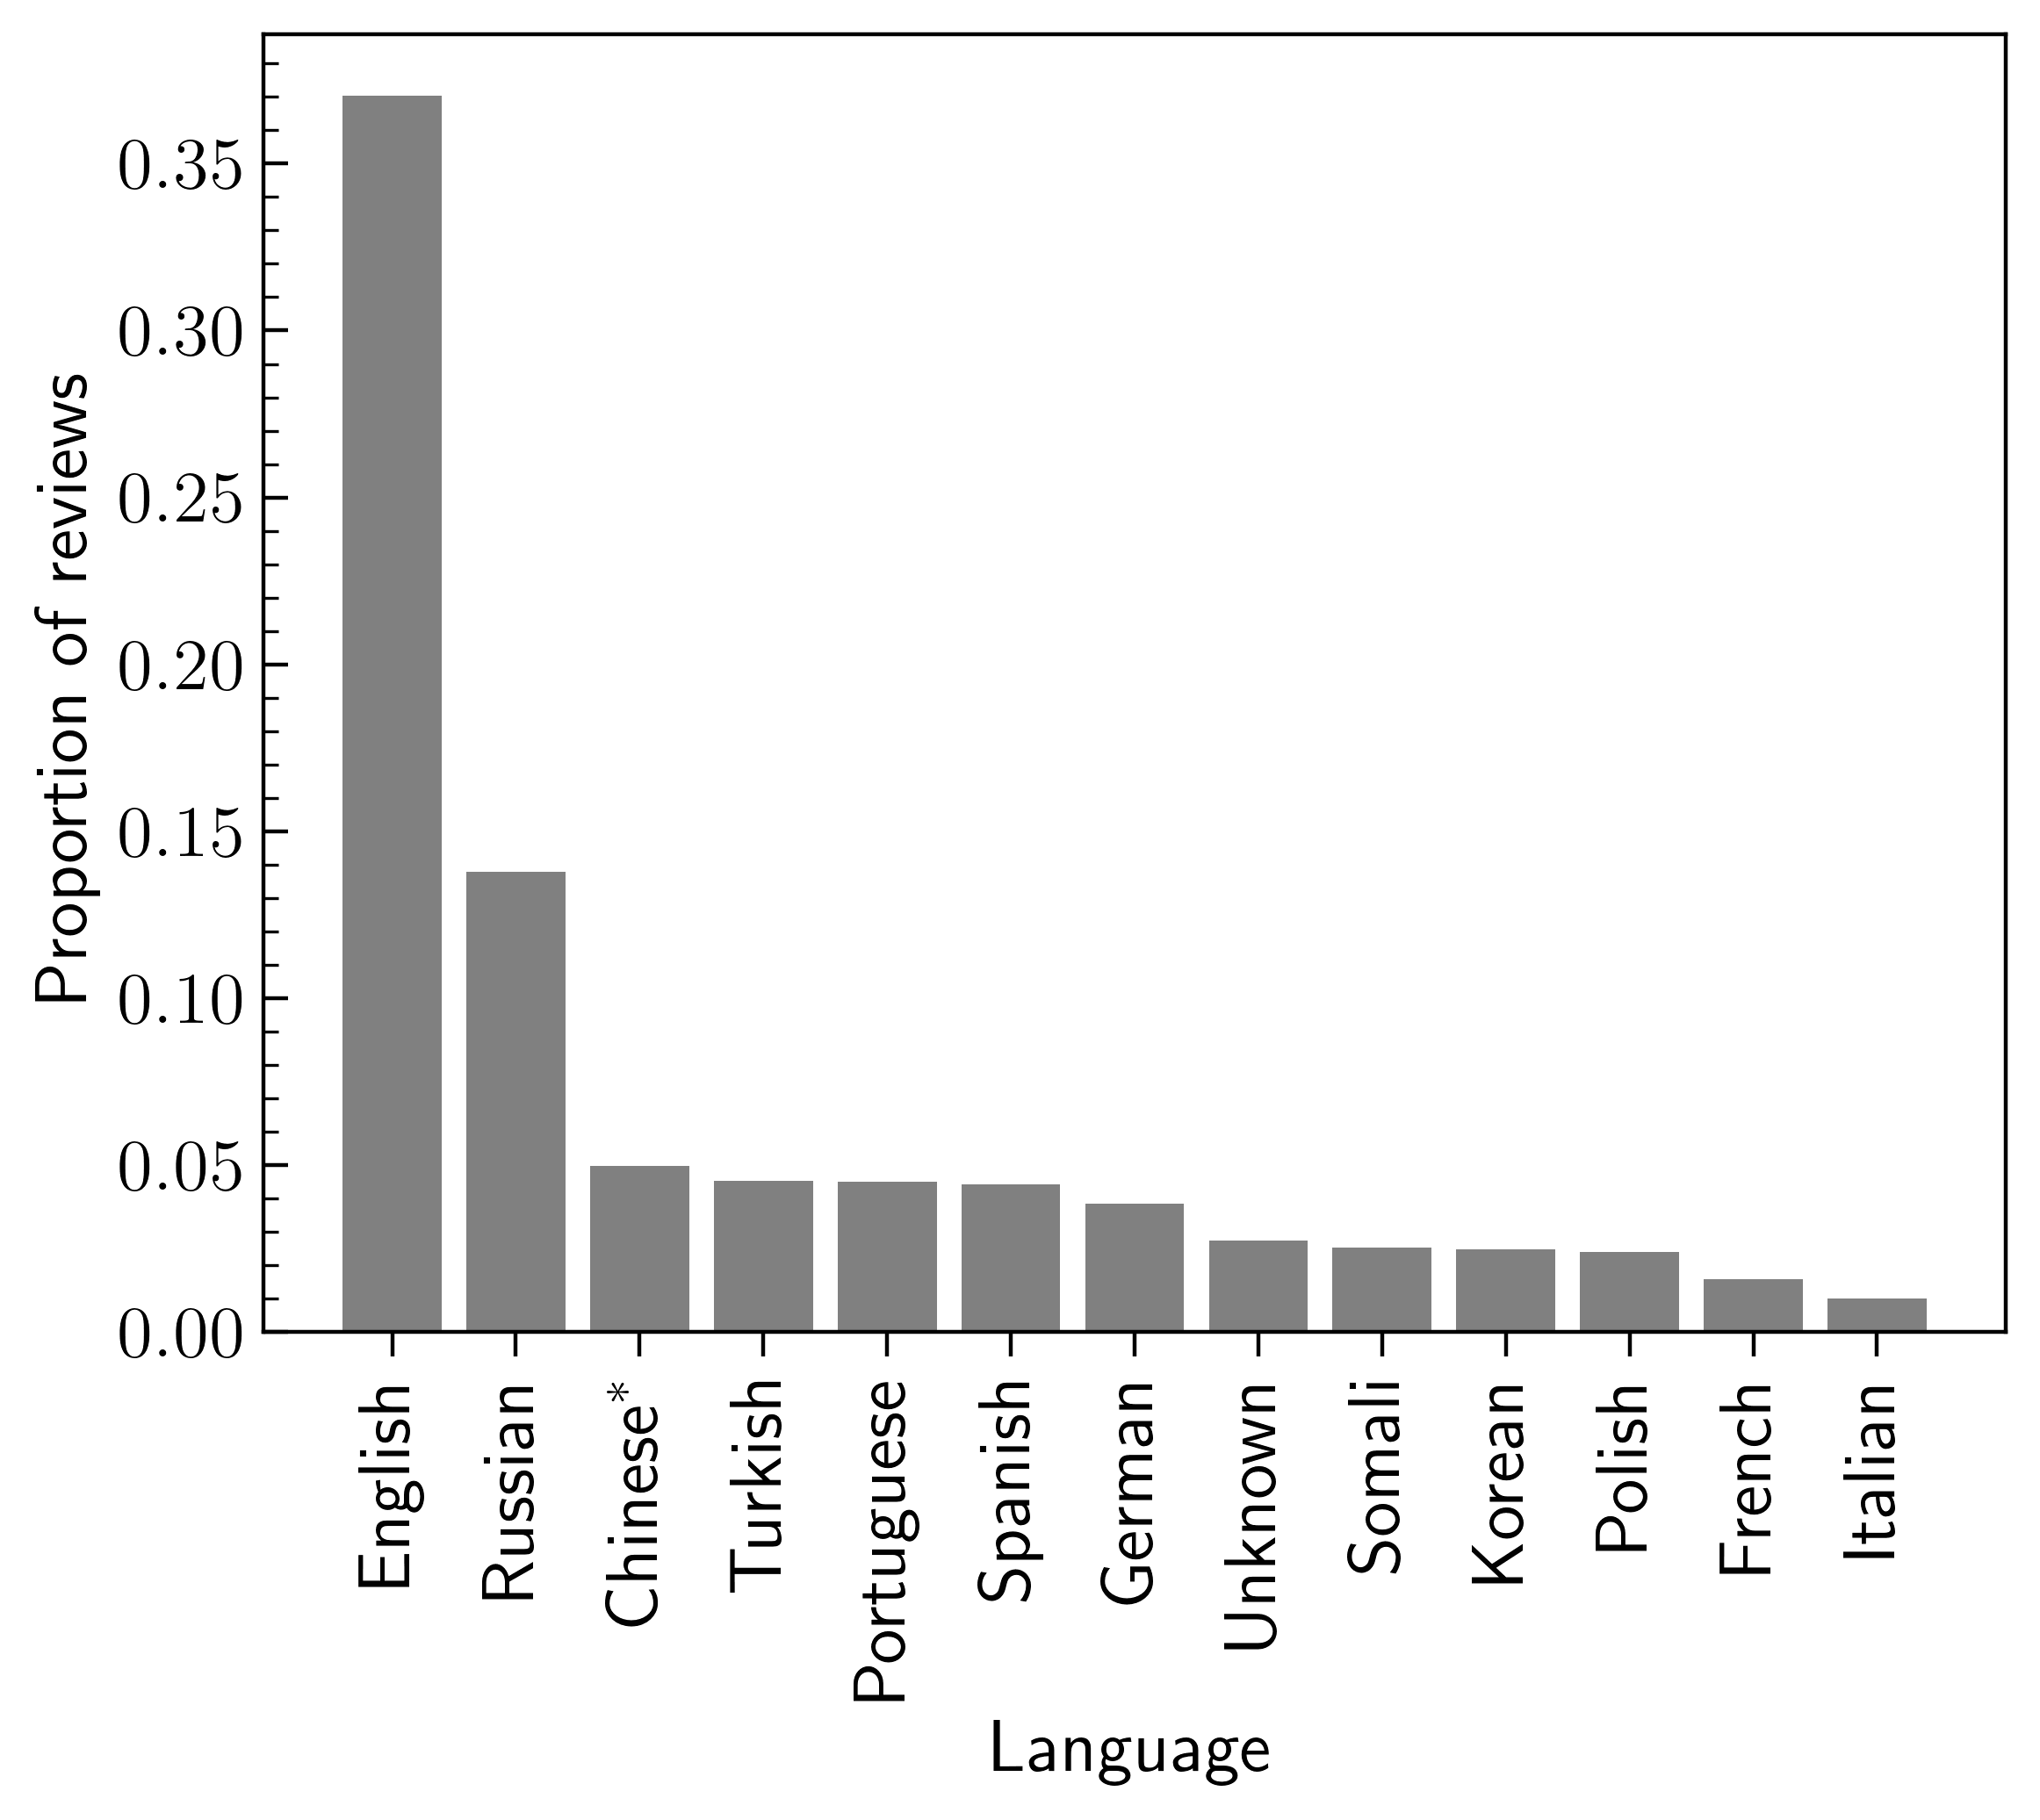
\includegraphics[width=\textwidth]{figures/03_dataset/12_bars_review_langs_min0.png}
        \caption{All reviews.}
        \label{fig:Dataset_BarsLangsMin1}
    \end{subfigure}
    \hfill
    \begin{subfigure}[ht]{0.49\textwidth}
        \centering
        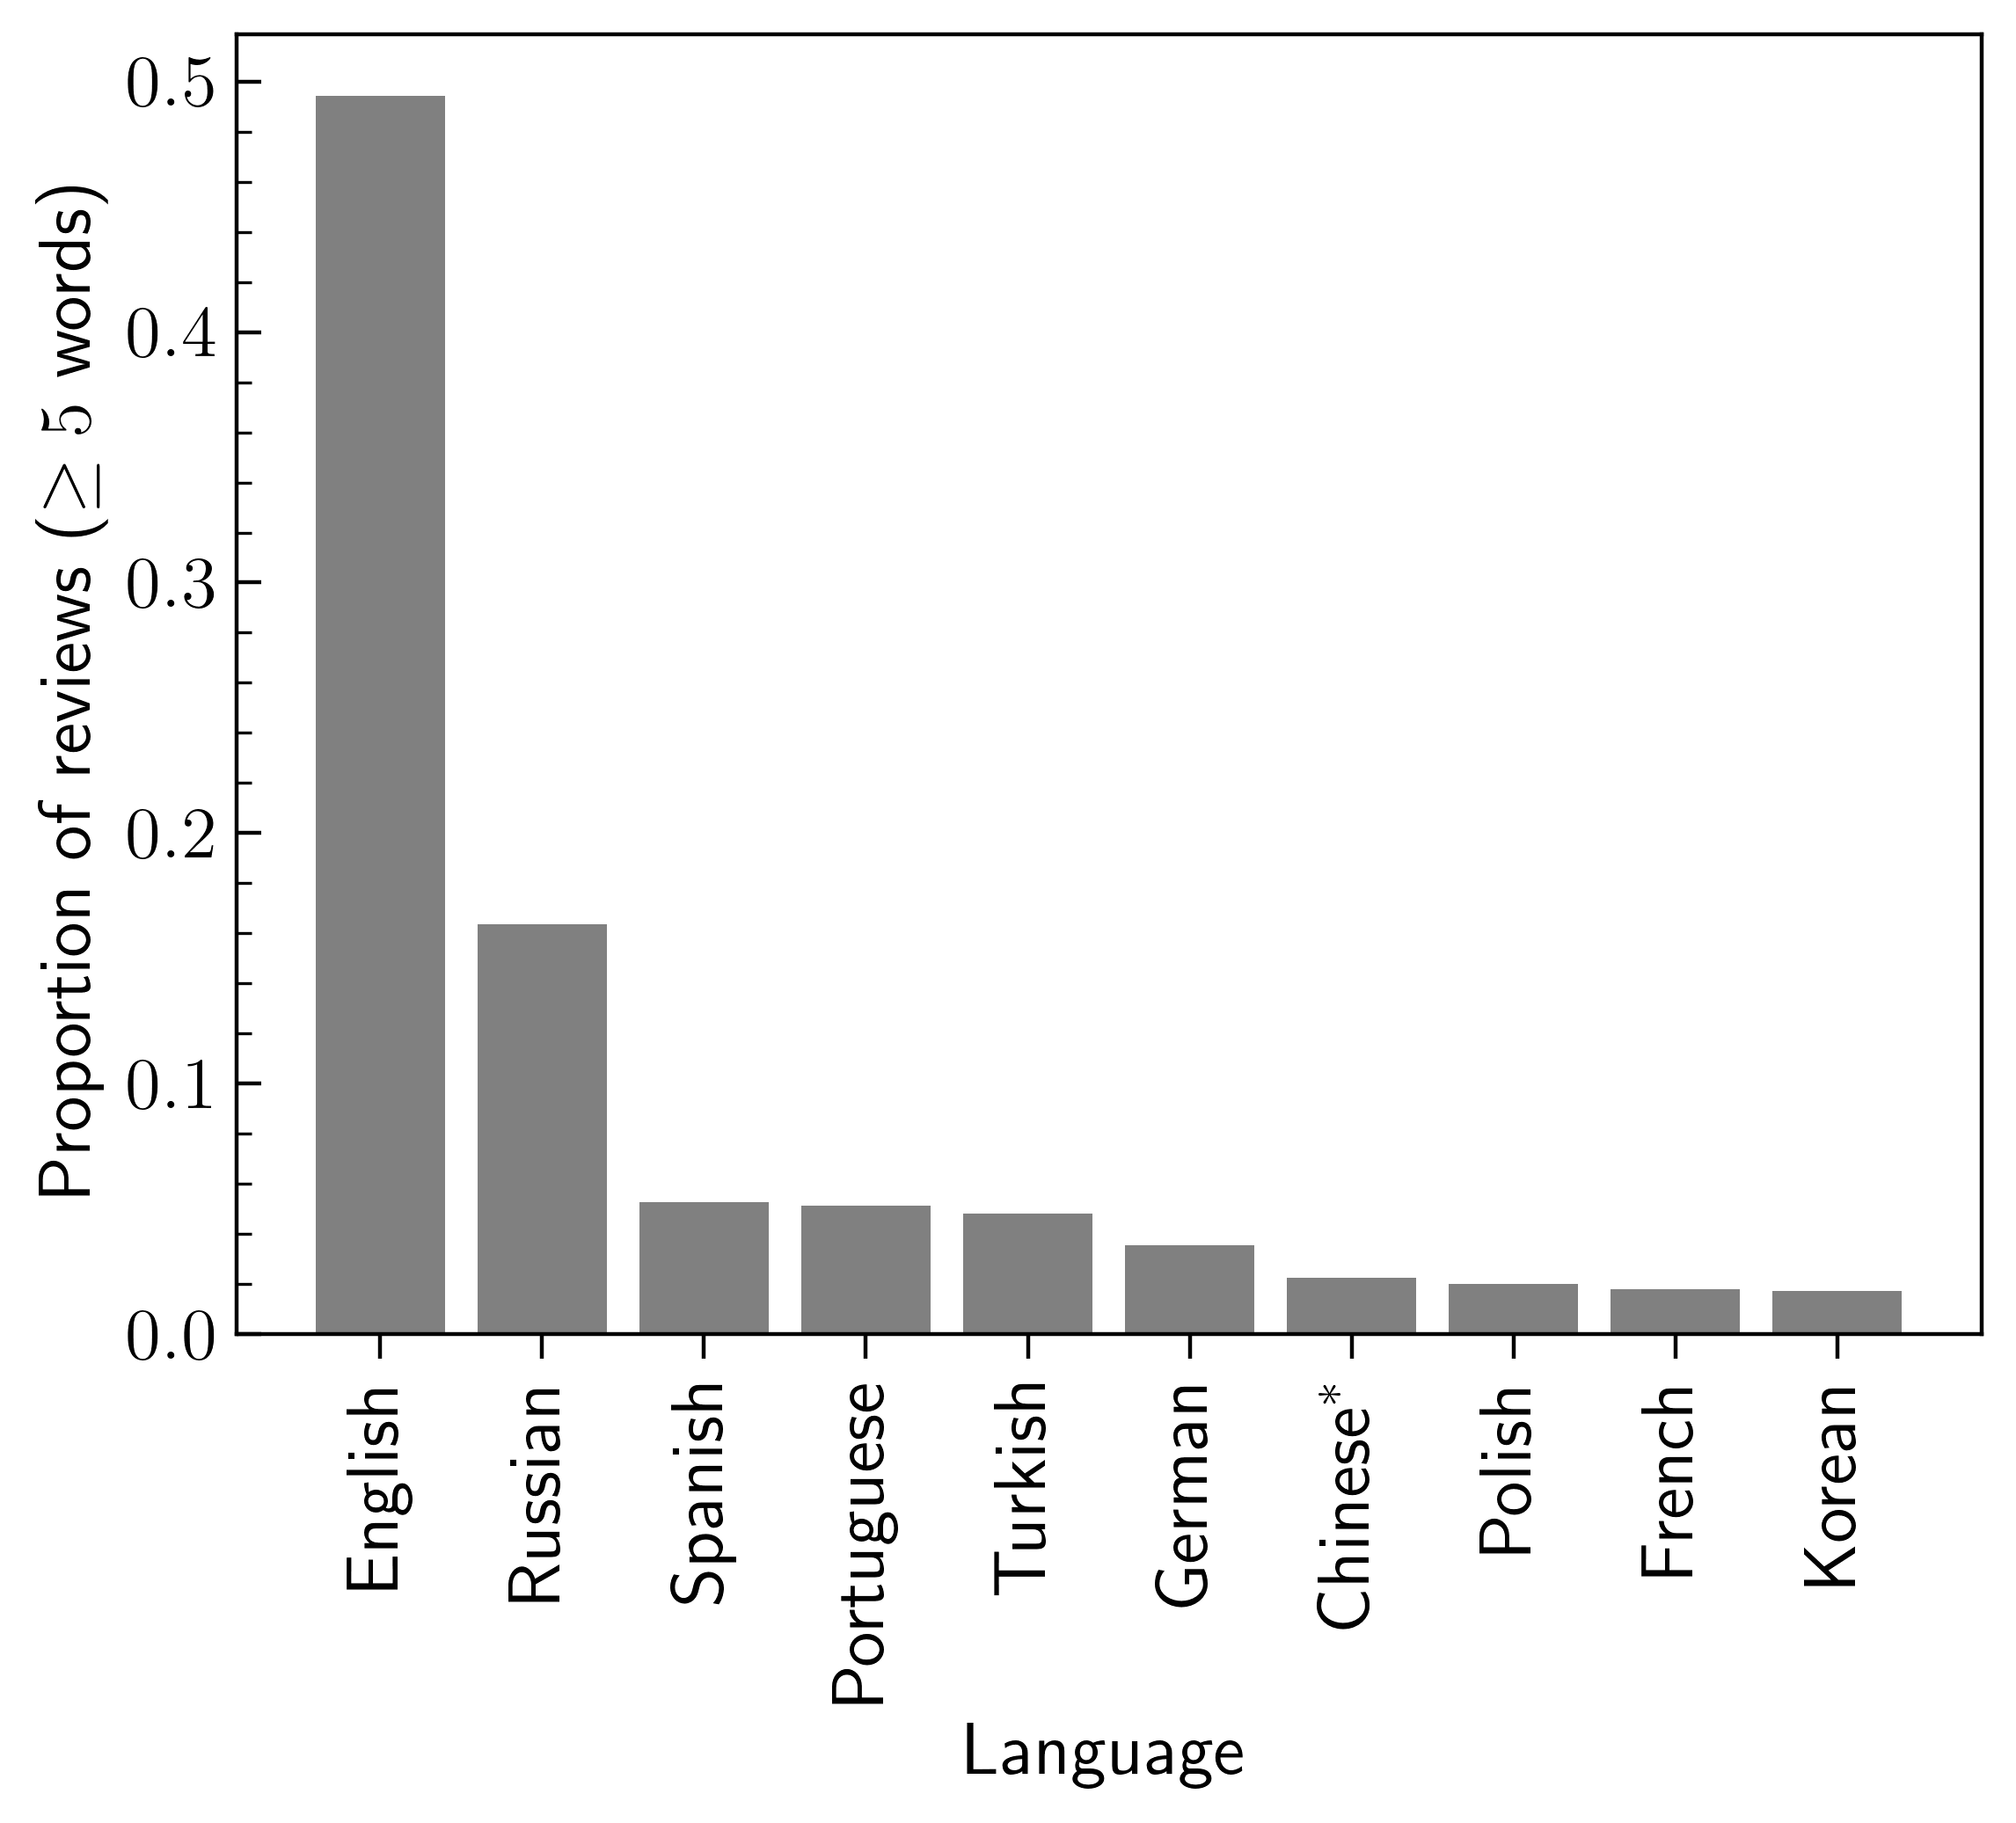
\includegraphics[width=\textwidth]{figures/03_dataset/13_bars_review_langs_min5.png}
        \caption{Reviews with at least five words.}
        \label{fig:Dataset_BarsLangsMin5}
    \end{subfigure}
    \caption{Language reviews were written in.}
    \label{fig:Dataset_BarsLangs}
\end{figure}

\footnotetext[1]{Chinese (Simplified)}

\subsection{Word Count}

The number of words in English-language reviews can be seen in Figure \ref{fig:Dataset_HistWordsEng}. Reviews with more than 277 words, 4.5\% of all such reviews, have been excluded from the histogram. The mean number of words in reviews is 62.7 (\textit{SD} = 134.3) and the median is 20. 25\% of reviews contain 8 words or fewer while 75\% contain 57 words or fewer.

\begin{figure}[ht]
    \centering
    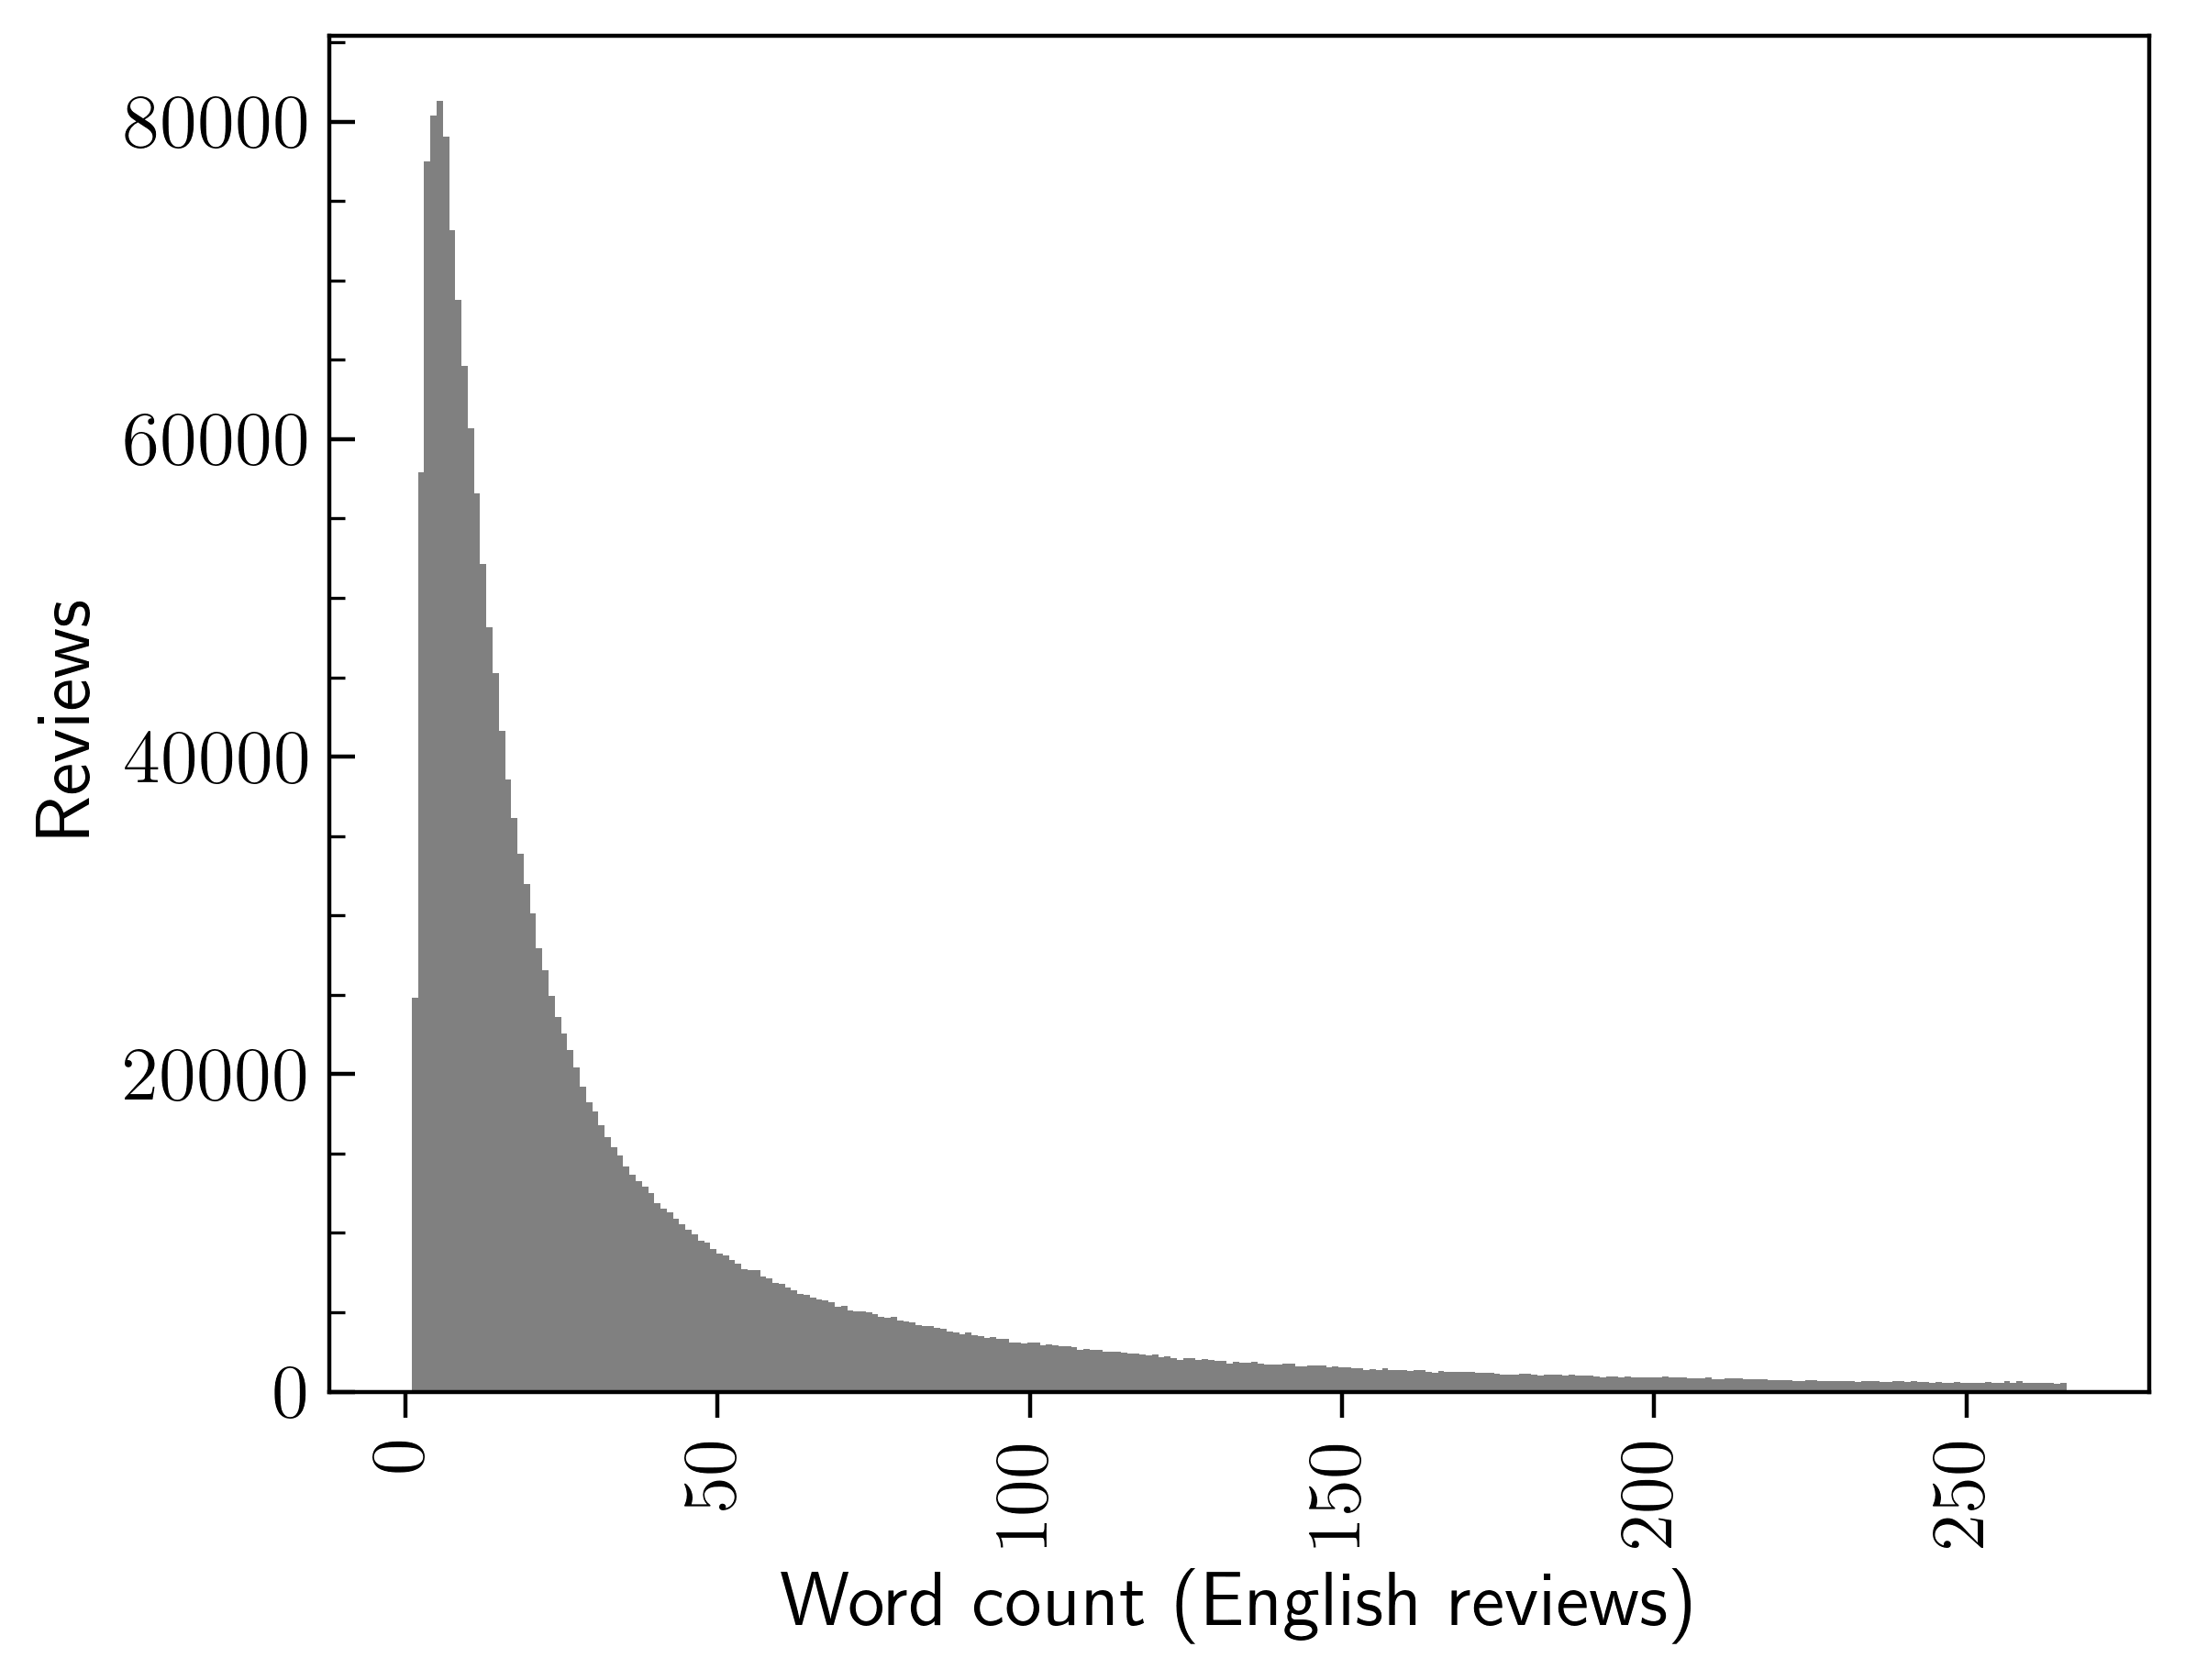
\includegraphics[scale=0.55]{figures/03_dataset/14_hist_review_words_en.png}
    \caption{Word count of English-language reviews.}
    \label{fig:Dataset_HistWordsEng}
\end{figure}

\chapter{Technical Background}

\section{BERT}

As discussed in section \ref{sec:LR_NLP}, BERT is a transformer-based NLP model developed by Google that achieved state-of-the-art results in numerous NLP tasks when it was published in 2018 \cite{Devlin2018_BERT}.

\subsection{Architecture}

The architecture of the BERT model is based around that of a transformer, a type of deep learning model that tries to simulate the human process of attention by assigning different weights to the tokens in a given input sample based on their apparent relevance \cite{Bahdanau2014_Attention} \cite{sabharwal2021bert}.

Textual inputs passed into BERT are tokenised and segmented, with each part of the input being represented as a function of its token, its segment and its position. A diagram illustrating this representation, taken from \cite{Devlin2018_BERT}, can be seen in Figure \ref{fig:Explain_BERTEmbeddings}. This method of representation allows the model to consider the context of each particular token with regard to the tokens that come before and after it \cite{sabharwal2021bert}.

\begin{figure}[ht]
    \centering
    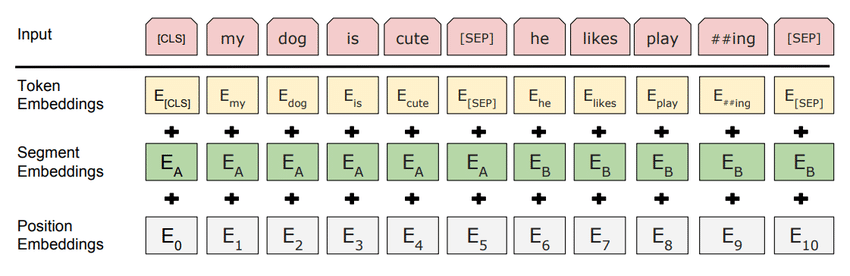
\includegraphics[scale=0.5]{figures/99_explanations/02_BERTEmbeddings.png}
    \caption{BERT input representation \cite{Devlin2018_BERT}.}
    \label{fig:Explain_BERTEmbeddings}
\end{figure}

These inputs are then fed through multiple encoding layers which try to determine how relevant different parts of the input are to each other through the aforementioned mechanism of attention \cite{AlammarTransformer}. The outputs from the encoding layer are passed through decoding layers before being passed through a softmax function to determine the final output \cite{Devlin2018_BERT}.

\subsection{Training}

The base BERT model was trained on over 3 billion words of data taken from English Wikipedia and BooksCorpus. The training process involved the completion of two tasks: masked language modelling and next sentence prediction. This initial training process is very time-consuming, generally taking multiple days to complete when using distributed cloud TPUs; although significant optimisations have been found that can reduce this time \cite{you2019large}.

\subsubsection{Masked Language Modelling}

This task involved the prediction of `masked' tokens in a sentence. Approximately 15\% of tokens in the dataset were replaced with \texttt{[MASK]} and the model's goal was to replace the masked tokens with the original terms \cite{Devlin2018_BERT}. For example, given the sentence ``I walked my \texttt{[MASK]} this morning'' as input, the model should produce the sentence ``I walked my dog this morning'' as output.

\subsubsection{Next Sentence Prediction}

This task involved the determination of whether or not two sentences ought to follow each other. The model would be given an initial sentence, \texttt{A}, and then given a second sentence, \texttt{B}, which, 50\% of the time directly followed \texttt{A} in the actual dataset and 50\% of the time was picked completely at random. The model's goal was to determine whether or not \texttt{B} actually followed \texttt{A} \cite{Devlin2018_BERT}. For example, given the sentences \texttt{A} = ``I walked my dog this morning'' and \texttt{B} = ``this is an unrelated sentence'', the model should determine that \texttt{B} does not follow \texttt{A}.

\subsection{Fine-tuning}

The fine-tuning process involves training the base BERT model on a smaller, specialised dataset, such as a collection of Steam reviews. This procedure is far less time-consuming than the initial training process and allows BERT to be quickly adapted to any NLP task \cite{Devlin2018_BERT}.

\subsection{DistilBERT}

The DistilBERT model \cite{sanh2019distilbert} is a pre-trained language representation model that is based on BERT but has been reduced in size by 40\% through the process of knowledge distillation, a process that reduces the size of a machine learning model without diminishing its predictive validity \cite{hinton2015distilling}. The resulting model, according to the authors, is 60\% faster than BERT and ``retains 97\% of its language understanding capabilities''.

\subsection{Exact Models Used}

Two pre-trained DistilBERT models were used over the course of this project: \texttt{distilbert-base-uncased} \cite{HuggingFaceEng} for fine-tuning with English samples and \texttt{distilbert-base-multilingual-cased} \cite{HuggingFaceMulti} for fine-tuning with multilingual samples. Both of these models were taken from Hugging Face \cite{wolf2019huggingface}. 

\section{Text Processing}

\subsection{Preprocessing}

Text data is often preprocessed before it is fed into a model. This can involve the conversion of the text to lowercase, particularly when the text is written in English; the splitting of the sentence into tokens; the removal of stop words; and the construction of $n$-grams from the remaining tokens.

\subsubsection{Tokenisation}

Tokenisation is the process by which a sample of text is split into a list of its component words or tokens, this is usually done based on the presence of punctuation marks, eg periods or commas, and spaces.

\subsubsection{Stop words}

Stop words are a set of very common words in a language, such as `the' or `and' in English, that tend to be filtered out or ignored in the process of text processing. This is based on the assumption that they carry very little useful information regarding any particular sample of text. Different languages have different sets of stop words and there is no universally agreed upon list of stop words for any particular language.

\subsubsection{N-grams}

$N$-grams are sets of $n$ consecutive tokens taken from a sample of text. For example, the set of $n$-grams of length 2, called bigrams, in a sentence would consist of a tuple for each consecutive pair of words. $N$-grams of length 1 are called unigrams while $n$-grams of length 3 are called trigrams.

\subsubsection{Examples}

Some examples of the above processes are given in Table \ref{tab:Explain_TextProc}.

\begin{table}[ht]
    \centering
    \begin{tabular}{l l}
        \toprule
        \textbf{Process} & \textbf{Result} \\\midrule
        Original & `Be quiet, the baby is sleeping.'\\
        Lowercased & `be quiet, the baby is sleeping.'\\
        Tokenised & `be', `quiet', `the', `baby', `is', `sleeping'\\
        Stop words removed & `quiet', `baby', `sleeping'\\
        Unigrams & (`quiet'), (`baby'), (`sleeping')\\
        Bigrams & (`quiet baby'), (`baby sleeping')\\
        Trigrams & (`quiet baby sleeping')\\
        \bottomrule\\
    \end{tabular}
    \caption{Examples of text preprocessing techniques applied in succession.}
    \label{tab:Explain_TextProc}
\end{table}

\subsection{Vectorisation}

Once a sample of text has been preprocessed it can be vectorised, a process that involves the mapping of its tokens to numerical values.

\subsubsection{Bag-of-words}

A simple example of text vectorisation is the bag-of-words model which tracks the particular tokens that were present in a sample as well as the frequency with which each token occurred. It's worth noting that this vectorisation model disregards the order in which tokens occurred in the text; however, when the technique is applied to $n$-grams, certain word orderings can be somewhat preserved. The set of distinct tokens that occur in all of the text samples is called the vocabulary and each token in the vocabulary is also mapped to a numerical value beginning at 0 and counting up. An example of bag-of-words vectorisation is given in Table \ref{tab:Explain_BOW}.

\begin{table}[ht]
    \centering
    \begin{tabular}{l l}
        \toprule
        \textbf{Process} & \textbf{Result} \\\midrule
        Original & `Be quiet, the baby is sleeping. The dog is also sleeping.'\\
        Preprocessed (unigrams) & `quiet', `baby', `sleeping', `dog', `also' `sleeping'\\
        Vectorised & $\begin{bmatrix} \text{`quiet'} & 1\\ \text{`baby'} & 1\\ \text{`sleeping'} & 2\\ \text{`dog'} & 1\\ \text{`also'} & 1\\ \end{bmatrix} \longrightarrow \begin{bmatrix} 1&1&2&1&1\\ \end{bmatrix}$\\
        \bottomrule\\
    \end{tabular}
    \caption{Example of bag-of-words vectorisation applied to a sentence}
    \label{tab:Explain_BOW}
\end{table}

\subsubsection{TF-IDF}

TF-IDF is a statistic used to weight the vectorised term (token) counts in each sample according to the frequency with which the term in question occurs in all of the samples in the dataset. The weights are then normalised using the Euclidean norm. For a given text sample, $s$, and a particular term, $t$, in a dataset containing $n$ total samples, the formula for calculating the TF-IDF weighting, taken from the documentation for \cite{pedregosa2011scikit}, is as follows:

\begin{equation*}
    v_{t,s} = \mathrm{tf}(t, s) \left( \log{\frac{n}{\mathrm{df}(t)}} + 1 \right)
\end{equation*}

where $\mathrm{tf}(t, s)$ is the number of times $t$ occurred in $s$ and $\mathrm{df}(t)$ is the number of samples $t$ appeared in. The normalisation formula, again taken from the documentation, is as follows:

\begin{equation*}
    v_{t,s}' = \frac{v_{t,s}}{\sqrt{\sum_{i=0}^n v_{t,i}^2}}
\end{equation*}

\section{Feature Scaling}

Feature scaling is a technique in machine learning preprocessing in which the values of numerical features, which might span any range, are normalised to fit into a finite defined range such as $[0,1]$ or $[-1,1]$. A very simple scaling technique, referred to as min-max scaling in the \cite{pedregosa2011scikit} documentation, involves the mapping of a list of values into the range $[0,1]$ with the maximum original value becoming 1, the minimum original value becoming 0 and the remaining values falling somewhere in between.

\subsection{Robust Scaling}

For data containing extreme or outlier values, techniques such as min-max scaling can produce poor results as most normalised values will be very similar with only the outliers being close to 0 or 1. A simplified description of robust scaling is that it scales values according to the interquartile range, ie the difference between the values in the 75th and 25th percentiles, as opposed to the median or the minimum and maximum values \cite{pedregosa2011scikit}. This technique reduces the influence of outliers on the resulting normalised values.

\section{Machine Learning Models}

\subsection{Baseline Classifiers}

Baseline or `dummy' classifiers are often used in comparison to trained models to better evaluate the trained models' performance. A simple baseline classifier is one that always predicts the most common label in the training data. A uniformly random classifier would predict any one of the labels in the training data at random, with each label having the same likelihood of being predicted. A slightly more advanced random classifier, which is better suited to data with more than two labels, would predict any one of the labels in the training data at random, with label probabilities being proportional to how often they actually occur in the data \cite{pedregosa2011scikit}.

\subsection{Naive Bayes Classifiers}

NB classifiers utilise Bayes' theorem to make predictions based on conditional probability, eg the probability that a sample should be classified as positive given a certain input feature. The meaning of the term `naive' comes from the fact that, when determining an overall classification based on numerous input features, conditional independence is naively assumed to exist between each set of input features which vastly reduces the amount of time and memory required to carry out calculations \cite{dangeti2017statistics}. As a result, NB classifiers tend to be very efficient \cite{pedregosa2011scikit}.

\subsubsection{Multinomial Naive Bayes}

A multinomial naive Bayes (MNB) classifier is a type of NB classifier that is particularly suited to text classification due to its modelling of the frequencies of terms in a sample, and the entire dataset, as a multinomial \cite{rennie2003tackling}.

\subsubsection{Complement Naive Bayes}

A complement naive Bayes (CNB) classifier is an adapted version of the MNB classifier which is better suited towards imbalanced datasets due to the fact that it is trained using the complement of the desired class, ie the probability that the given sample is \textit{not} a member of the desired class \cite{pedregosa2011scikit} \cite{rennie2003tackling}.

\subsection{Support Vector Machines}

Support vector machines (SVM), specifically linear SVMs, are a group of machine learning models that can be used for both classification and regression. When trained for classification, linear SVMs attempt to find a linear separation between both classes in the training data, using a hyperplane, while also maximising the distance between training points on the separation boundaries and the hyperplane itself \cite{dangeti2017statistics}. When more than two classes are present a one-vs-rest strategy is used to break the classification problem down into multiple binary classification problems \cite{pedregosa2011scikit}. An illustration of an SVM classifier can be seen in Figure \ref{fig:Explain_LSVC}.

\begin{figure}[ht]
    \centering
    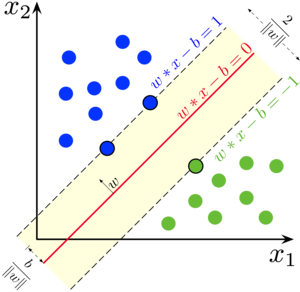
\includegraphics[scale=4]{figures/99_explanations/01_LSVC.png}
    \caption{Example of an optimal hyperplane found by an SVM classifier for two classes \cite{WikipediaLSVC}.}
    \label{fig:Explain_LSVC}
\end{figure}

When trained for regression, linear SVMs attempt to fit a hyperplane to the training data that contains the maximum number of data points \cite{smola2004tutorial}.

\subsubsection{Stochastic Gradient Descent}

Stochastic gradient descent (SGD) is an optimisation algorithm for minimising the cost function of a machine learning model, over numerous iterations, using approximations of the function's actual gradient calculated from multiple subsets of the training data. SGD is highly efficient and can be used for both classification and regression problems. SGD can be used in linear SVM classifiers and regressors \cite{pedregosa2011scikit}.

\subsection{Baselines Regressors}

As was the case with classifiers, baseline or `dummy' regressors are often used in comparison to trained models. Two simple examples of baseline regressors are those that always predict either the mean or the median of the values in the training data \cite{pedregosa2011scikit}.

\subsection{Ridge Regressors}

Ridge regression models use least squares regression combined with a regularisation penalty, which includes the sum of the squares of the regression coefficients in the cost function in order to reduce overfitting \cite{dangeti2017statistics}.

\section{Evaluation Metrics}

\subsection{Classification}

\subsubsection{True and Predicted Labels}

In a classification task involving two labels, positive and negative, predictions can be split into four categories depending on the true label and the predicted label of the item in question. These categories are shown in the confusion matrix in Table \ref{tab:Explain_ConfMat}.

\renewcommand\arraystretch{1.5}
\begin{table}[ht]
    \centering
    \begin{tabular}{l|l|c|c|}
        \multicolumn{2}{c}{} & \multicolumn{2}{c}{True}\\
        \cline{3-4}
        \multicolumn{2}{c|}{} & Positive & Negative\\
        \cline{2-4}
        \multirow{2}{*}{Predicted}& Positive & True positive (TP) & False positive (FP)\\
        \cline{2-4}
        & Negative & False negative (FN) & True negative (TN)\\
        \cline{2-4}
    \end{tabular}
    \caption{Confusion matrix for binary classification}
    \label{tab:Explain_ConfMat}
\end{table}

\subsubsection{Accuracy}

The accuracy of a classifier is the proportion of predicted labels that match the true labels:

\begin{equation*}
    \mathrm{Accuracy} = \frac{TP + TN}{TP + FP + TN + FN}
\end{equation*}

Accuracy can give a general overview of how well a classifier is performing but it can be a poor evaluation metric in datasets with an imbalanced number of positive and negative items.

\subsubsection{Precision and Recall}

The precision of a classifier is the ratio of true positive predictions to total positive predictions:

\begin{equation*}
    \mathrm{Precision} = \frac{TP}{TP + FP}
\end{equation*}

The recall of a classifier is the ratio of true positive predictions to total positive items:

\begin{equation*}
    \mathrm{Recall} = \frac{TP}{TP + FN}
\end{equation*}

Precision and recall, used in conjunction, can provide better insight into the predictive capability of a classifier, particularly when the dataset being used is imbalanced.

\subsubsection{$F_1$-score}

The $F_1$-score of a classifier is a measure of its overall accuracy using the harmonic mean of the precision and recall values:

\begin{equation*}
    F_1 = \frac{2 \cdot \mathrm{Precision} \cdot \mathrm{Recall}}{\mathrm{Precision} + \mathrm{Recall}}
\end{equation*}

The use of the harmonic mean of both values rather than the arithmetic mean ensures that higher $F_1$-scores, which indicate a better result, can only occur when both precision and the recall are high themselves.

\subsubsection{Receiver Operating Characteristic}

The receiver operating characteristic (ROC) curve compares the true positive rates (TPR) and false positive rates (FPR) of a classifier as its decision threshold is varied. The TPR is equivalent to the recall value while the FPR is the ratio of false positive predictions to total negative items:

\begin{equation*}
    \mathrm{FPR} = \frac{FP}{TN + FP}
\end{equation*}

The decision threshold of a classifier is the value at which a predicted probability score for a specific class is considered high enough to assign that class's label to the item being predicted. The decision threshold can range from 0 to 1, with 0.5 generally being the default value.

\subsubsection{Area Under the Curve}

The area under the curve (AUC) is simply the total area underneath an ROC curve. The AUC can range from 0 to 1 with larger values indicating a better classifier. The AUC can be considered a numerical overview or summary of an ROC curve.

\subsection{Regression}

\subsubsection{Mean Squared Error}

The mean squared error (MSE) is a metric used in regression to compute the average squared difference between predicted values and true values. Given a sample of $n$ items, with the true and predicted values of the $i$-th sample being denoted as $y_i$ and $\hat{y}_i$, respectively, the equation used to compute the MSE, taken from the documentation for \cite{pedregosa2011scikit}, is as follows:

\begin{equation*}
    \mathrm{MSE} = \frac{1}{n} \sum_{i=1}^n (y_i - \hat{y}_i)^2
\end{equation*}

Smaller MSE values are indicative of a more accurate model.

\subsubsection{Negative Mean Squared Error}

The negative MSE (NMSE) is functionally identical to the MSE except for the fact that it is negative meaning that larger values, ie those closer to 0, are better.

\subsubsection{$R^2$ Score}

The $R^2$ score, also called the coefficient of determination, is a measure of how well a model has been fitted to the dataset. Given a sample of $n$ items, with the true and predicted values of the $i$-th sample being denoted as $y_i$ and $\hat{y}_i$, respectively, and $\bar{y}$ being the arithmetic mean of all true values, the equation used to compute $R^2$, again taken from the documentation for \cite{pedregosa2011scikit}, is as follows:

\begin{equation*}
    R^2 = 1 - \frac{\sum_{i=1}^n (y_i - \hat{y}_i)^2}{\sum_{i=1}^n (y_i - \bar{y})^2}
\end{equation*}

A higher $R^2$ score indicates a more accurate model, with the best possible score being 1. A score of 0 would be considered a baseline, ie a model that always predicted the arithmetic mean of the values, although negative scores are possible.

\chapter{Design and Implementation} \label{sec:DI}

This chapter will discuss, in detail, the methods used and the approaches taken when implementing solutions to the two primary tasks this dissertation is concerned with: the prediction of various review features using only the review text and the identification of users who best represent the population of reviewers, as a whole, through the content of their written reviews.

\section{Review Feature Prediction} \label{sec:DI_RF}

In this section, the process of selecting and training optimal machine learning models with the goal of predicting three features of a given review will be discussed. The review features being predicted are its polarity, how many helpfulness votes it received and the length of time the reviewer spent playing the game. The machine learning models that will be tested are BERT, specifically two pretrained DistilBERT models; MNB and CNB classifiers; linear SVMs for classification and regression, both with SGD and without; a ridge regressor; and multiple baseline classifiers and regressors.

\subsection{Dataset Sampling} \label{sec:DI_RF_Sampling}

Due to the time and memory-consuming nature of the model training procedure in machine learning, especially when considering neural networks like BERT, it would be unfeasible to utilise the entirety of the dataset, which consists of over 10 million reviews, in the model training and testing processes. Instead, numerous samples of the dataset, each containing exactly 100 thousand reviews, were prepared and used to train the predictive models.

Only reviews consisting of at least one word, determined by the process outlined in section \ref{sec:Dataset_RT_Langs}, were included when preparing the dataset samples. The language that a review was written in was considered a determining factor in relation to how well the trained models would be able to accurately predict the selected review features. As such, separate samples were prepared for reviews written in English\footnote{Reviews that were classified as English with a confidence of at least 70\% by the language detection algorithm discussed in \ref{sec:Dataset_RT_Langs} were included in the English-language samples.} and reviews written in any language (including English). Also of interest was the potential effect that the length of the review text, ie the word count, might have on the accuracy of the trained models' predictions. As such, separate samples were prepared for reviews that contained 50 words or more, referred to as `long' reviews; reviews that contained fewer than 50 words, referred to as `short' reviews; and reviews containing any number of words.

Several samples were also prepared solely for the task of review polarity prediction. Due to the imbalanced nature of the dataset with regard to review polarity, 85\% of reviews are positive while only 15\% of reviews are negative, and, since this task is a classification problem, separate samples were prepared, containing equal numbers of positive and negative reviews in order to more accurately determine how well the trained models were performing.

The names and characteristics of all of the prepared data samples are given in Table \ref{tab:DI_RF_Datasets}.

\begin{table}[ht]
    \centering
    \begin{tabular}{l|l l l l}
        \toprule
        \textbf{Sample Name} & \textbf{Language} & \textbf{Length} & \textbf{Balanced} & \textbf{Size}\\\midrule
        \texttt{eng\_eq\_any} & English & Any & Yes & 100k\\
        \texttt{eng\_eq\_short} & English & Short & Yes & 100k\\
        \texttt{eng\_eq\_long} & English & Long & Yes & 100k\\
        \texttt{any\_eq\_any} & Multilingual & Any & Yes & 100k\\
        \texttt{any\_eq\_short} & Multilingual & Short & Yes & 100k\\
        \texttt{any\_eq\_long} & Multilingual & Long & Yes & 100k\\
        \texttt{eng\_any\_any} & English & Any & No & 100k\\
        \texttt{eng\_any\_short} & English & Short & No & 100k\\
        \texttt{eng\_any\_long} & English & Long & No & 100k\\
        \texttt{any\_any\_any} & Multilingual & Any & No & 100k\\
        \texttt{any\_any\_short} & Multilingual & Short & No & 100k\\
        \texttt{any\_any\_long} & Multilingual & Long & No & 100k\\
        \bottomrule
    \end{tabular}
    \caption{Dataset samples and their characteristics for review feature prediction.}
    \label{tab:DI_RF_Datasets}
\end{table}

\subsection{Polarity} \label{sec:DI_RF_Pol}

\subsubsection{BERT}

\paragraph{Data Splitting}

Each dataset sample was split into three sets: training (80\% of the sample), validation (10\% of the sample) and test (10\% of the sample). The training set was used to fine-tune the BERT model, the validation set was used to evaluate the trained model after each epoch and the test set was used to determine the overall quality of the fully trained model.

\paragraph{Preprocessing}

Very little preprocessing needed to be done to the data before it was passed into the BERT model for training. Tokenisation was done using the pretrained tokenisers that were provided with both the English-language and multilingual DistilBERT models. The tokenised input data, alongside the output polarity data, were converted to tensors, before being used to fit the BERT classifier.

\paragraph{Hyperparameter Tuning}

Optimal training parameters were selected for all of the BERT models used to predict review polarity by testing numerous combinations of parameters on a model trained using the \texttt{eng\_eq\_any} sample. Individually applying the hyperparameter tuning process to each of the dataset samples, even if it may have led to slightly better results for those samples, would have been far too time-consuming to carry out.

The learning rate of the Adam optimiser, which is used by the classifier, was originally considered as a tunable parameter; however, experimenting with its value did not lead to any improvements and, as such, it was not considered in the final approach. The two parameters which were settled on were the batch size and the number of epochs the model was to be trained for. The parameter values that were considered can be seen in Table \ref{tab:DI_RF_Pol_BERTHP}.

\begin{table}[ht]
    \centering
    \begin{tabular}{l l}
        \toprule
        \textbf{Hyperparameter} & \textbf{Values}\\\midrule
        Batch size & $16, 32, 64$\\
        Epochs & $2, 3, 4$\\
        \bottomrule\\
    \end{tabular}
    \caption{BERT hyperparameters for review polarity.}
    \label{tab:DI_RF_Pol_BERTHP}
\end{table}

The training and validation accuracies of the trained models for each combination of hyperparameters can be seen in Figure \ref{fig:DI_RF_Pol_BERTHP}.

\begin{figure}[ht]
    \centering
    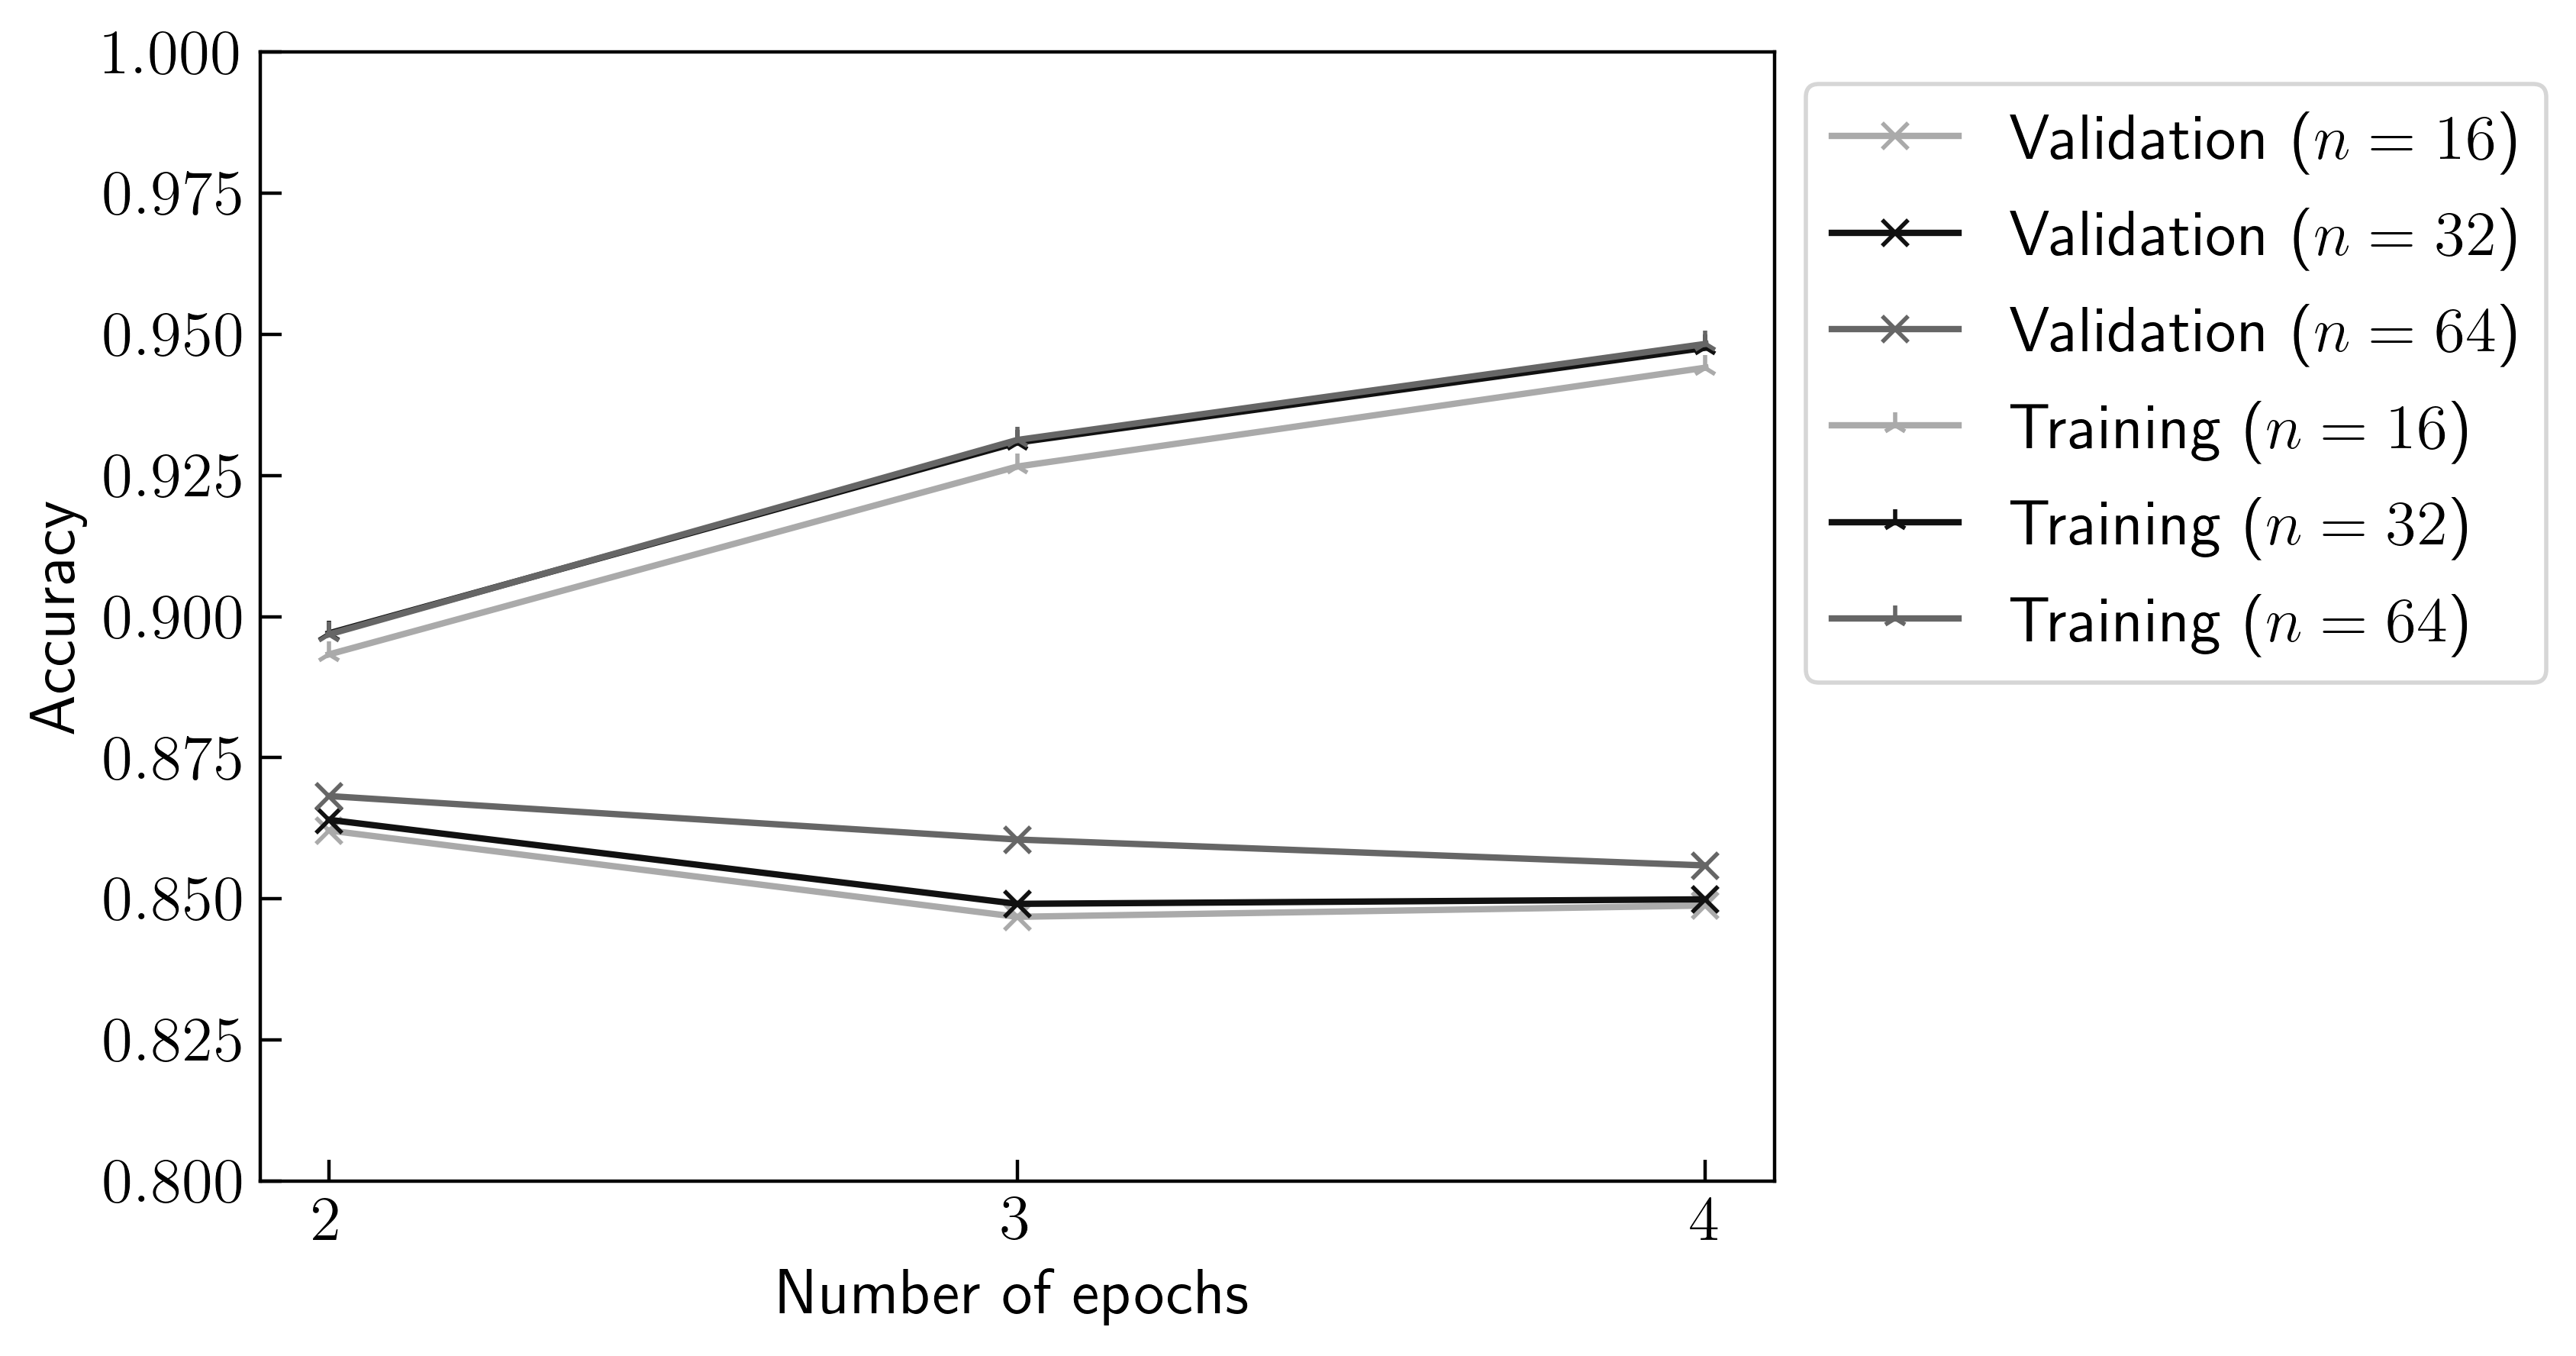
\includegraphics[scale=0.7]{figures/05_impl/01_rfp/01_pol/plot_hyperparams_bert.png}
    \caption{BERT hyperparameter tuning results for review polarity ($n$ is batch size).}
    \label{fig:DI_RF_Pol_BERTHP}
\end{figure}

Based on these results it is clear that the classifiers begin to overfit the training data after 2 epochs as the training accuracy begins to increase at the expense of the validation accuracy. The models trained with a batch size of 64 also appear to perform the strongest and, as such, the combination of 2 epochs and a batch size of 64 will be used when training and testing BERT models for the other dataset samples.

\paragraph{Training Procedure}

BERT models were trained and validated for all 12 dataset samples using the optimal hyperparameters. Samples containing English reviews were trained using the pretrained \texttt{distilbert-base-uncased} model while multilingual samples were trained using the \texttt{distilbert-base-multilingual-cased} model. Their performance was then tested using the test sets of their respective samples. The results of these tests will be discussed, in detail, in section \ref{sec:Res_RF_Pol}.

\subsubsection{Other Models}

\paragraph{Data Splitting}

In contrast to the procedure utilised when training BERT models, the dataset samples were split into two sets rather than three: training (90\% of the sample) and test (10\% of the sample). The training results were gathered using the mean accuracy of 5-fold cross-validation performed on the training set as opposed to the validation accuracy taken from the BERT training process. The test results were gathered in the same manner as the BERT test results were gathered.

\paragraph{Preprocessing}

Unlike with BERT, significant preprocessing needed to be applied to the review text data before it could be passed into a model for training. The steps involved in this process are as follows:

\begin{enumerate}
    \item Convert the text to lowercase\footnote{Only for English-language reviews.}.
    \item Replace all non-word characters\footnote{Any Unicode character that is not a letter used in words in any language.} with spaces.
    \item Split the text into words based on spaces.
    \item Remove any stopwords.
    \item Join the remaining words back together and remove repeated spaces.
    \item Vectorise the text.
    \item Apply TF-IDF weightings to the vectorised text.
\end{enumerate}

The text was also processed into various sets of $n$-grams before being used in model training; however, this process will be discussed in the following section. The list of stopwords used was provided by Python's NLTK library \cite{bird2009natural} which contains stopword lists for 24 different languages.

\paragraph{Hyperparameter Tuning}

As was the case with BERT, optimal hyperparameters for each model were selected based on the results gathered for the \texttt{eng\_eq\_any} sample due to the time-consuming nature of the training process.

Regardless of the model being used, the review text was converted into sets of $n$-grams of varying sizes and ranges\footnote{The $n$-gram range of $(1, 2)$, for example, would consist of all unigrams and bigrams taken from the text.}. For the MNB, CNB and SGD classifiers, the $\alpha$ parameter was varied. For the LSVC, the $C$ parameter was varied. Parameter ranges were chosen so as to provide a large amount of variance between results so that the optimal parameters for each model could be accurately selected. The parameter values that were considered can be seen in Table \ref{tab:DI_RF_Pol_BaseHP}.

\begin{table}[ht]
    \centering
    \begin{tabular}{l l l}
        \toprule
        \textbf{Model} & \textbf{Hyperparameter} & \textbf{Values}\\\midrule
        All & $n$-gram range & $(1, 2), (1, 3), (1, 4)$\\
        MNB & $\alpha$ & $0.01, 0.1, 1, 10$\\
        CNB & $\alpha$ & $0.01, 0.1, 1, 10$\\
        SGD & $\alpha$ & $10^{-4}, 10^{-5}, 10^{-6}$\\
        LSVC & $C$ & $0.01, 0.1, 1, 10$\\
        \bottomrule\\
    \end{tabular}
    \caption{Other model hyperparameters for review polarity.}
    \label{tab:DI_RF_Pol_BaseHP}
\end{table}

Two baseline classifiers were also used for comparison: one which predicted a random class and one which predicted the most frequent class. The mean cross-validation accuracies for each combination and model can be seen in Figure \ref{fig:DI_RF_Pol_BaseHP}. The standard deviations of the cross-validation accuracies were also gathered; however, they were all found to be insignificantly small and, as such, have not been included in the plot.

\begin{figure}[ht]
    \hspace*{-0.3in}
    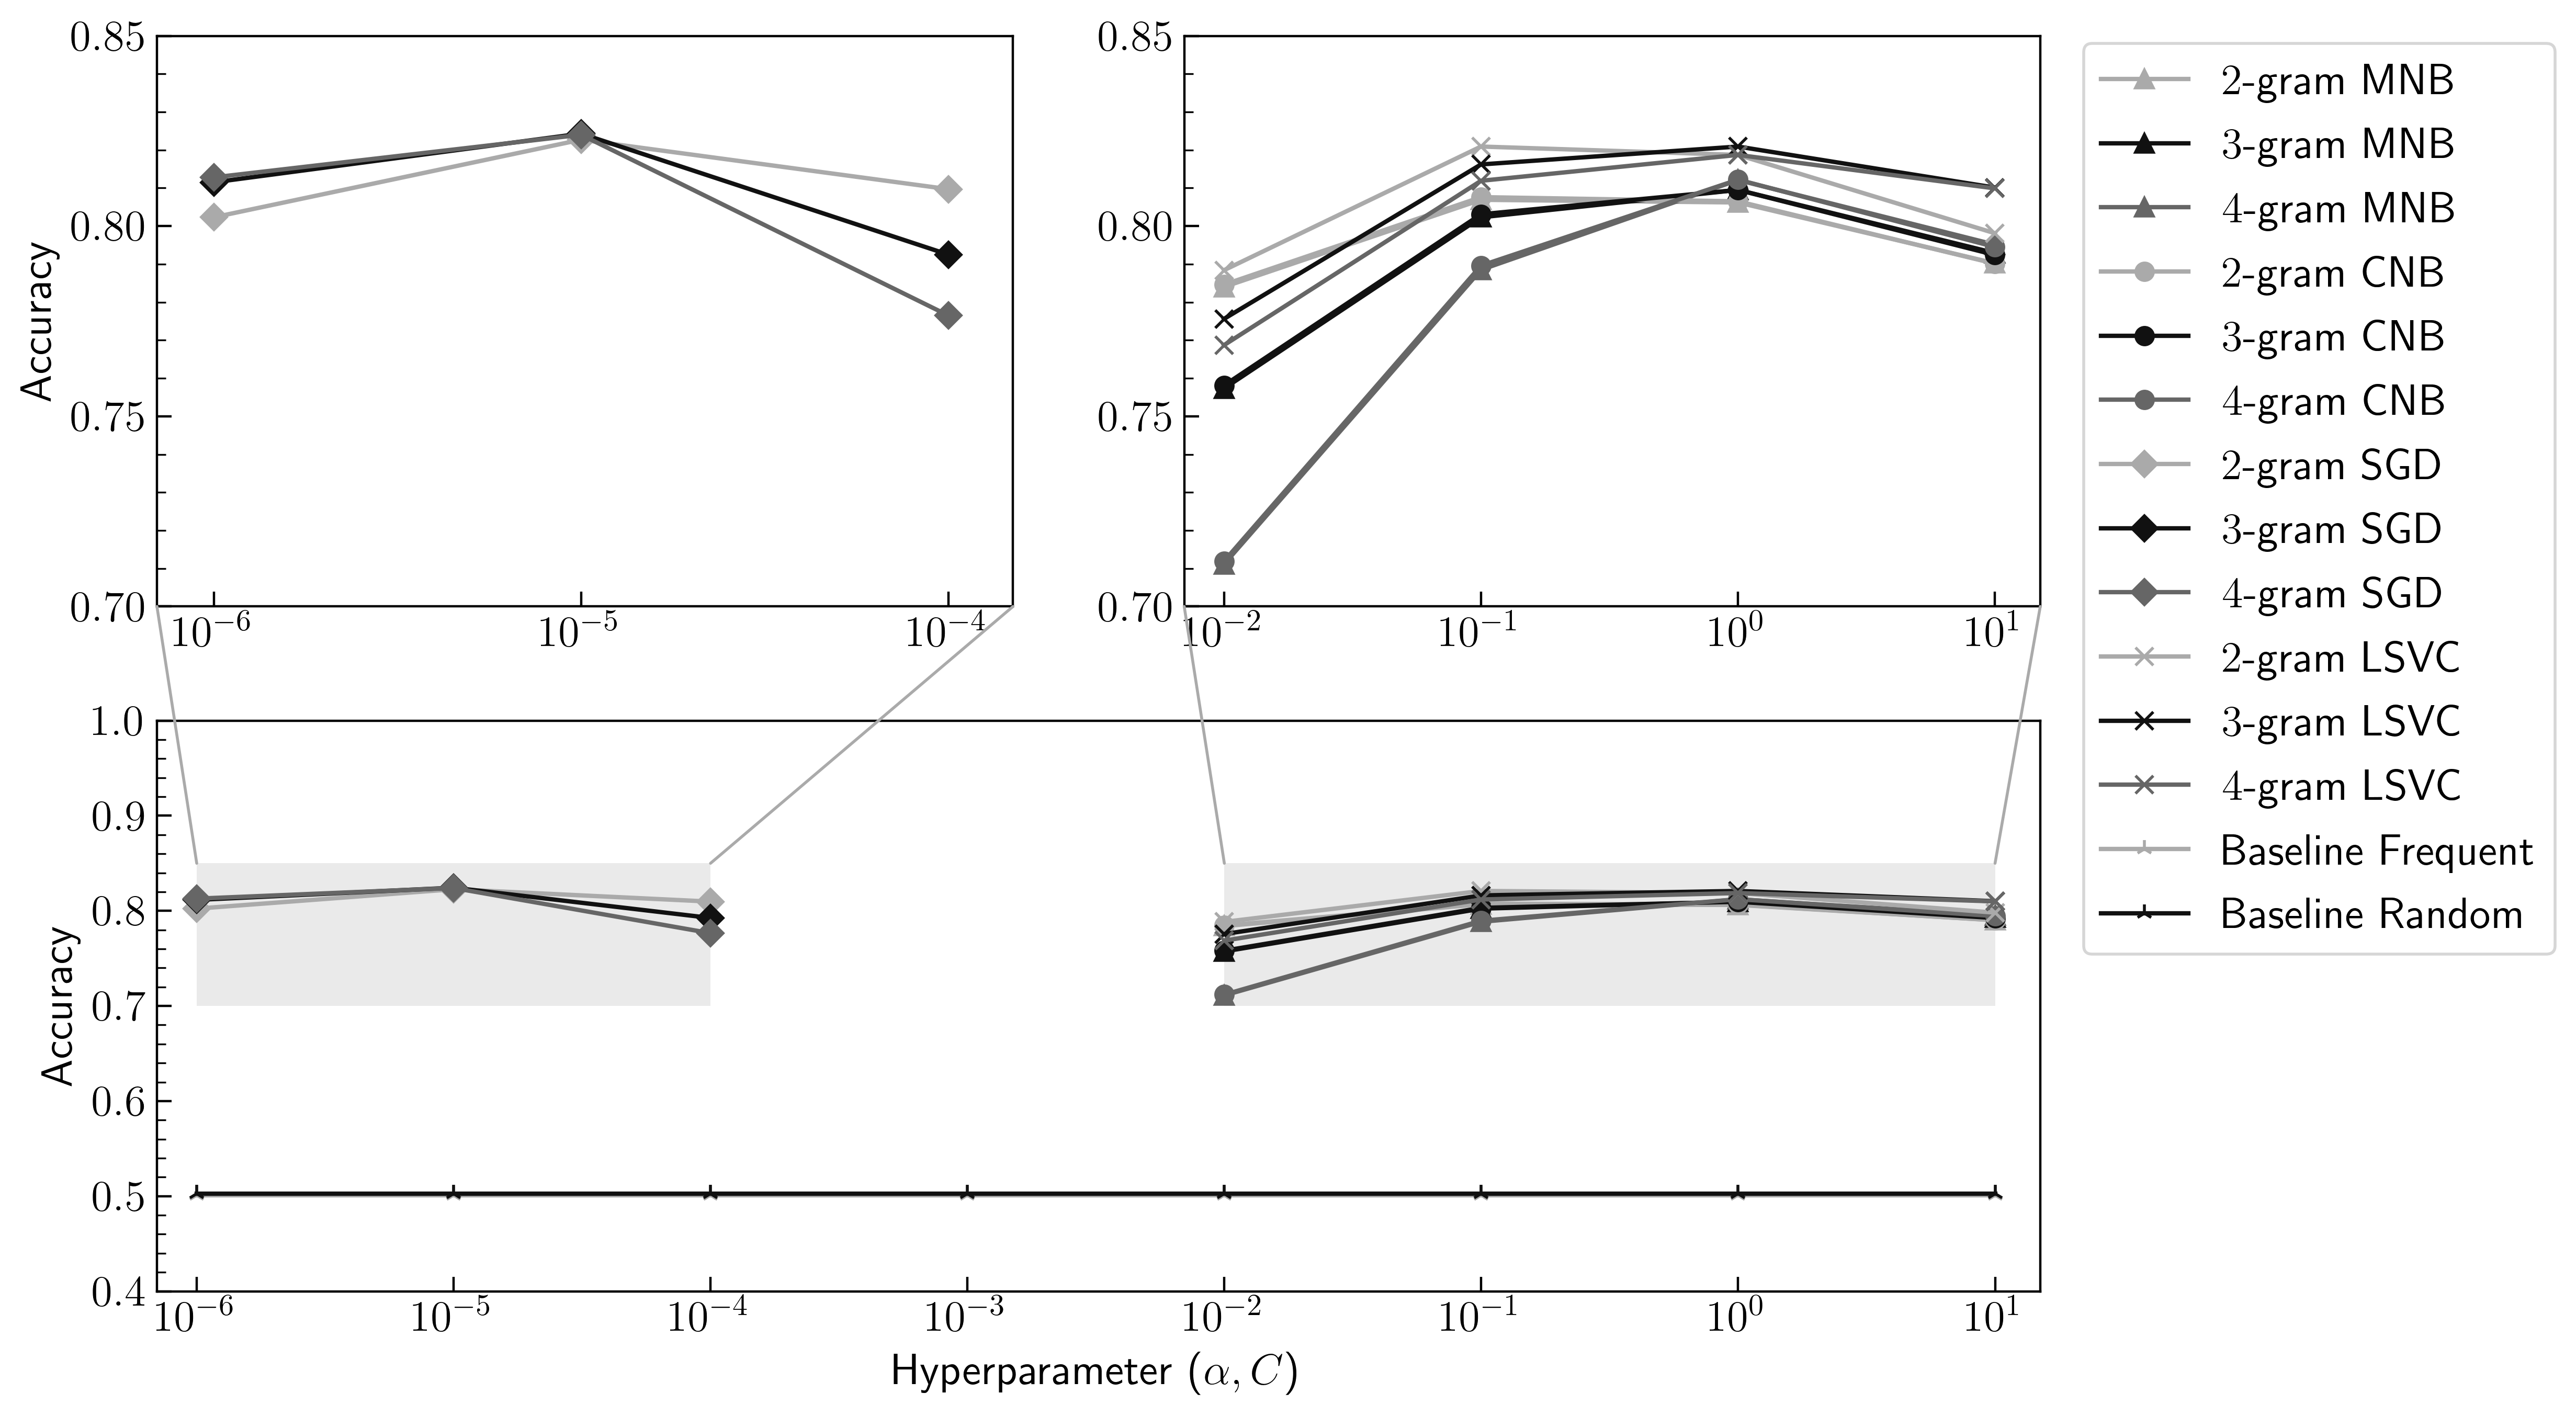
\includegraphics[scale=0.55]{figures/05_impl/01_rfp/01_pol/plot_hyperparams_base.png}
    \caption{Other model hyperparameter tuning results for review polarity.}
    \label{fig:DI_RF_Pol_BaseHP}
\end{figure}

Based on these results it seems that, for each SGD classifier, the parameter value of $\alpha=10^{-5}$ is optimal. The $n$-gram range of $(1, 3)$ also seems to have the best performance for that $\alpha$, though not by much. For the LSVC, a parameter value of $C=1$ with an $n$-gram range of $(1, 3)$ appears to be the best choice, although $C=0.1$ with an $n$-gram range of $(1, 2)$ performs almost as well.

Both of the NB classifiers seem to produce very similar results for each choice of $\alpha$ and $n$-gram range. In each case, it is clear that a parameter value of $\alpha=1$ with an $n$-gram range of $(1,4)$ is the best performing combination.

\paragraph{Training Procedure}

Each of the optimal classifiers was trained on all 12 dataset samples and their performance was then tested using the test sets of their respective samples. The test results will be discussed, and compared to the BERT results, in section \ref{sec:Res_RF_Pol}.

\subsection{Votes} \label{sec:DI_RF_Votes}

The process of training the machine learning models to predict the number of helpfulness votes that reviews received was very similar to the process used to predict their polarity. One key difference in the procedure was that the balanced dataset samples, ie those with 50\% positive and 50\% negative reviews, were not relevant to the task and were, as a result, not included.

\subsubsection{BERT}

\paragraph{Data Splitting}

The dataset samples were split into the same three sets, with the same proportions, that were mentioned for the BERT model in section \ref{sec:DI_RF_Pol}.

\paragraph{Preprocessing}

As was also discussed previously, very little preprocessing needed to be done to the text data before being passed into the BERT model. However, a robust scaler was used to map the number of votes each review received down to a limited range centred around 0. A robust scaler was used due to the presence of outliers in the dataset.

\paragraph{Hyperparameter Tuning}

Optimal training parameters were selected for all of the BERT models based on the results gathered for the \texttt{eng\_any\_any} sample. The same combinations of batch size and training epochs were tested for the prediction of review votes as were tested for the prediction of review polarity. These values can be seen, again, in Table \ref{tab:DI_RF_Votes_BERTHP}.

\begin{table}[ht]
    \centering
    \begin{tabular}{l l}
        \toprule
        \textbf{Hyperparameter} & \textbf{Values}\\\midrule
        Batch size & $16, 32, 64$\\
        Epochs & $2, 3, 4$\\
        \bottomrule\\
    \end{tabular}
    \caption{BERT hyperparameters for review votes.}
    \label{tab:DI_RF_Votes_BERTHP}
\end{table}

The NMSE loss for both the training and validation sets can be seen in Figure \ref{fig:DI_RF_Votes_BERTHP}.

\begin{figure}[ht]
    \centering
    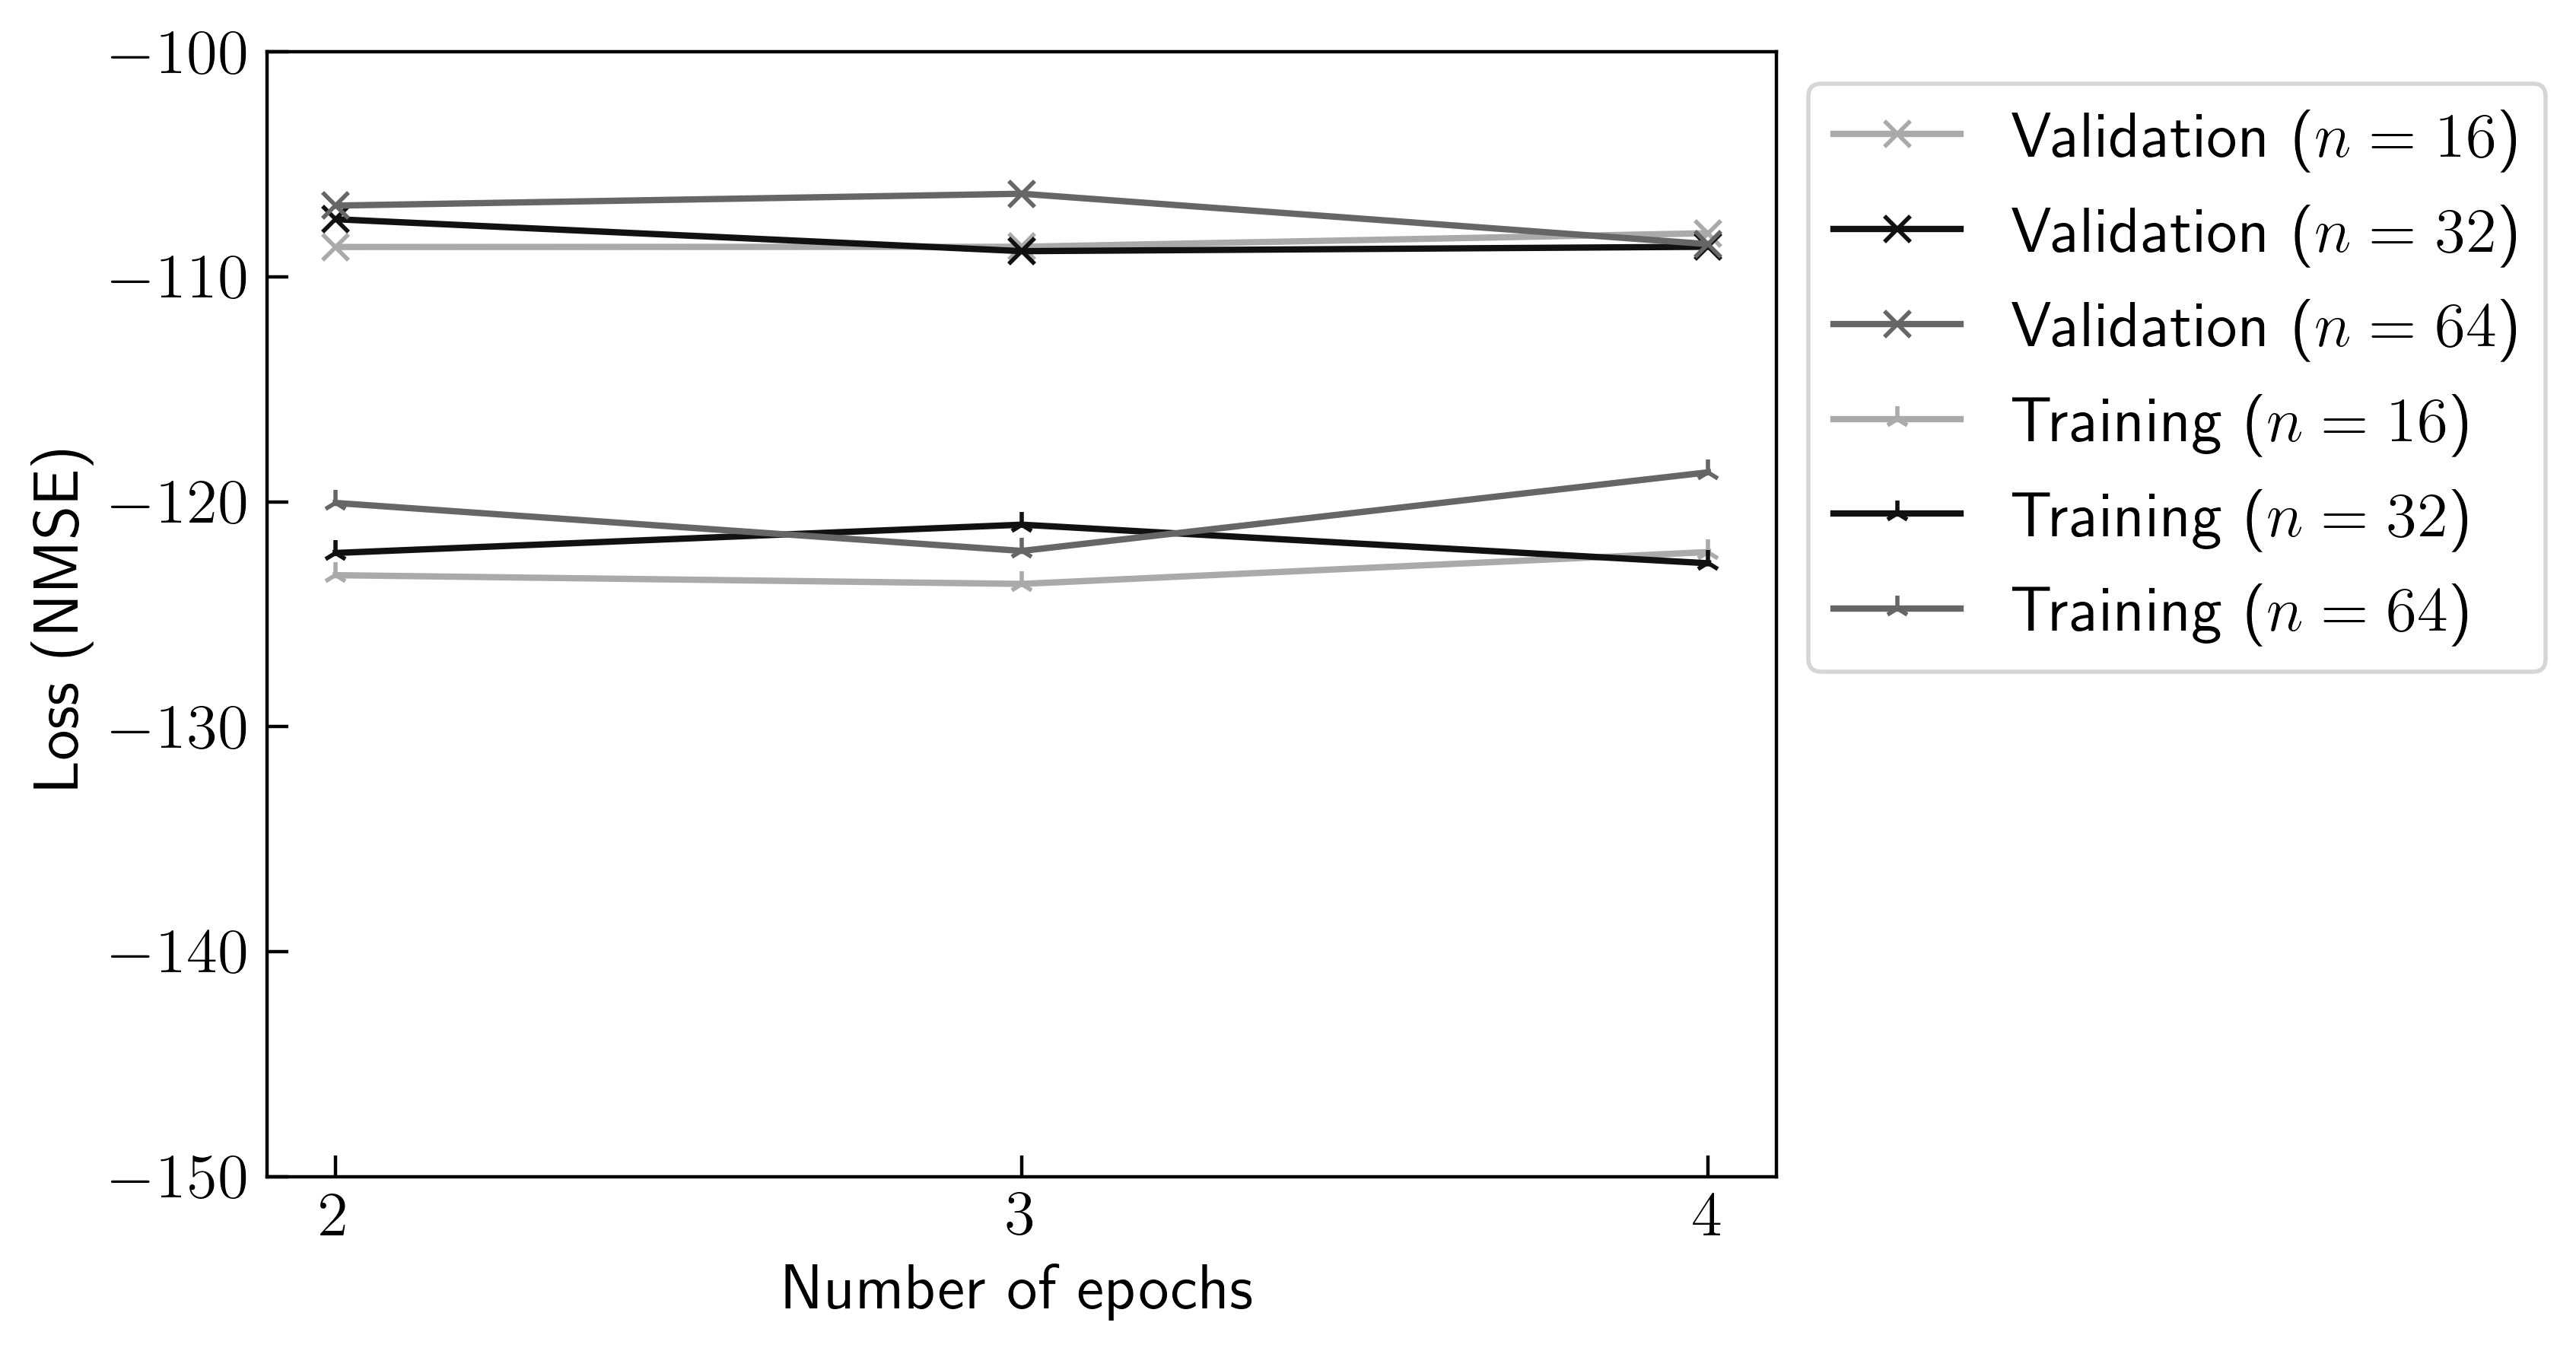
\includegraphics[scale=0.7]{figures/05_impl/01_rfp/02_votes/plot_hyperparams_bert.png}
    \caption{BERT hyperparameter tuning results for review votes ($n$ is batch size).}
    \label{fig:DI_RF_Votes_BERTHP}
\end{figure}

Interestingly, based on these results, it seems that the trained models might be underfitting the training data due to the superior performance of the model against the validation set. Regardless, the best results were produced when a batch size of 64 was used. For a batch size of 64, the results for both 2 and 3 training epochs are almost identical and so, in the interest of reducing training time, 2 epochs would appear to be the optimal choice.

\paragraph{Training Procedure}

The same training procedure was used for the prediction of reviews votes as was used for the prediction of review polarity with the only significant difference being the number of dataset samples being considered.

\subsubsection{Other Models}

\paragraph{Data Splitting}

The dataset splitting procedure was identical to the one outlined for the other models in section \ref{sec:DI_RF_Pol}.

\paragraph{Preprocessing}

The numerous preprocessing steps that were applied to the review text when predicting polarity were also applied here. An additional preprocessing step, discussed already in this section, was the use of a robust scaler to map the number of votes down to a limited range while accounting for outliers.

\paragraph{Hyperparameter Tuning}

Optimal hyperparameters were selected for each model based on the results gathered for the \texttt{eng\_any\_any} sample. The review text was, again, converted into sets of $n$-grams of varying sizes and ranges. For the SGD and ridge regressors, the $\alpha$ parameter was varied. For the LSVR, the $C$ parameter was varied. The methodology used to select parameter ranges, to provide varied results to better identify optimal values, was again applied. The parameter values that were considered can be seen in Table \ref{tab:DI_RF_Votes_BaseHP}.

\begin{table}[ht]
    \centering
    \begin{tabular}{l l l}
        \toprule
        \textbf{Model} & \textbf{Hyperparameter} & \textbf{Values}\\\midrule
        All & $n$-gram range & $(1, 2), (1, 3), (1, 4)$\\
        Ridge & $\alpha$ & $0.01, 0.1, 1, 10$\\
        SGD & $\alpha$ & $10^{-3}, 10^{-4}, 10^{-5}, 10^{-6}$\\
        LSVR & $C$ & $0.01, 0.1, 1, 10$\\
        \bottomrule\\
    \end{tabular}
    \caption{Other model hyperparameters for review votes.}
    \label{tab:DI_RF_Votes_BaseHP}
\end{table}

Two baseline regressors were also used for comparison: one which predicted the mean number of scaled votes and one which predicted the median number of scaled votes. The mean cross-validation NMSE losses, along with the standard deviations, can be seen in Figure \ref{fig:DI_RF_Votes_BaseHP}. In order to improve the clarity of the plots in Figure \ref{fig:DI_RF_Votes_BaseHP}, some results have been offset slightly on the x-axis.

\begin{figure}[ht]
    \hspace*{-0.3in}
    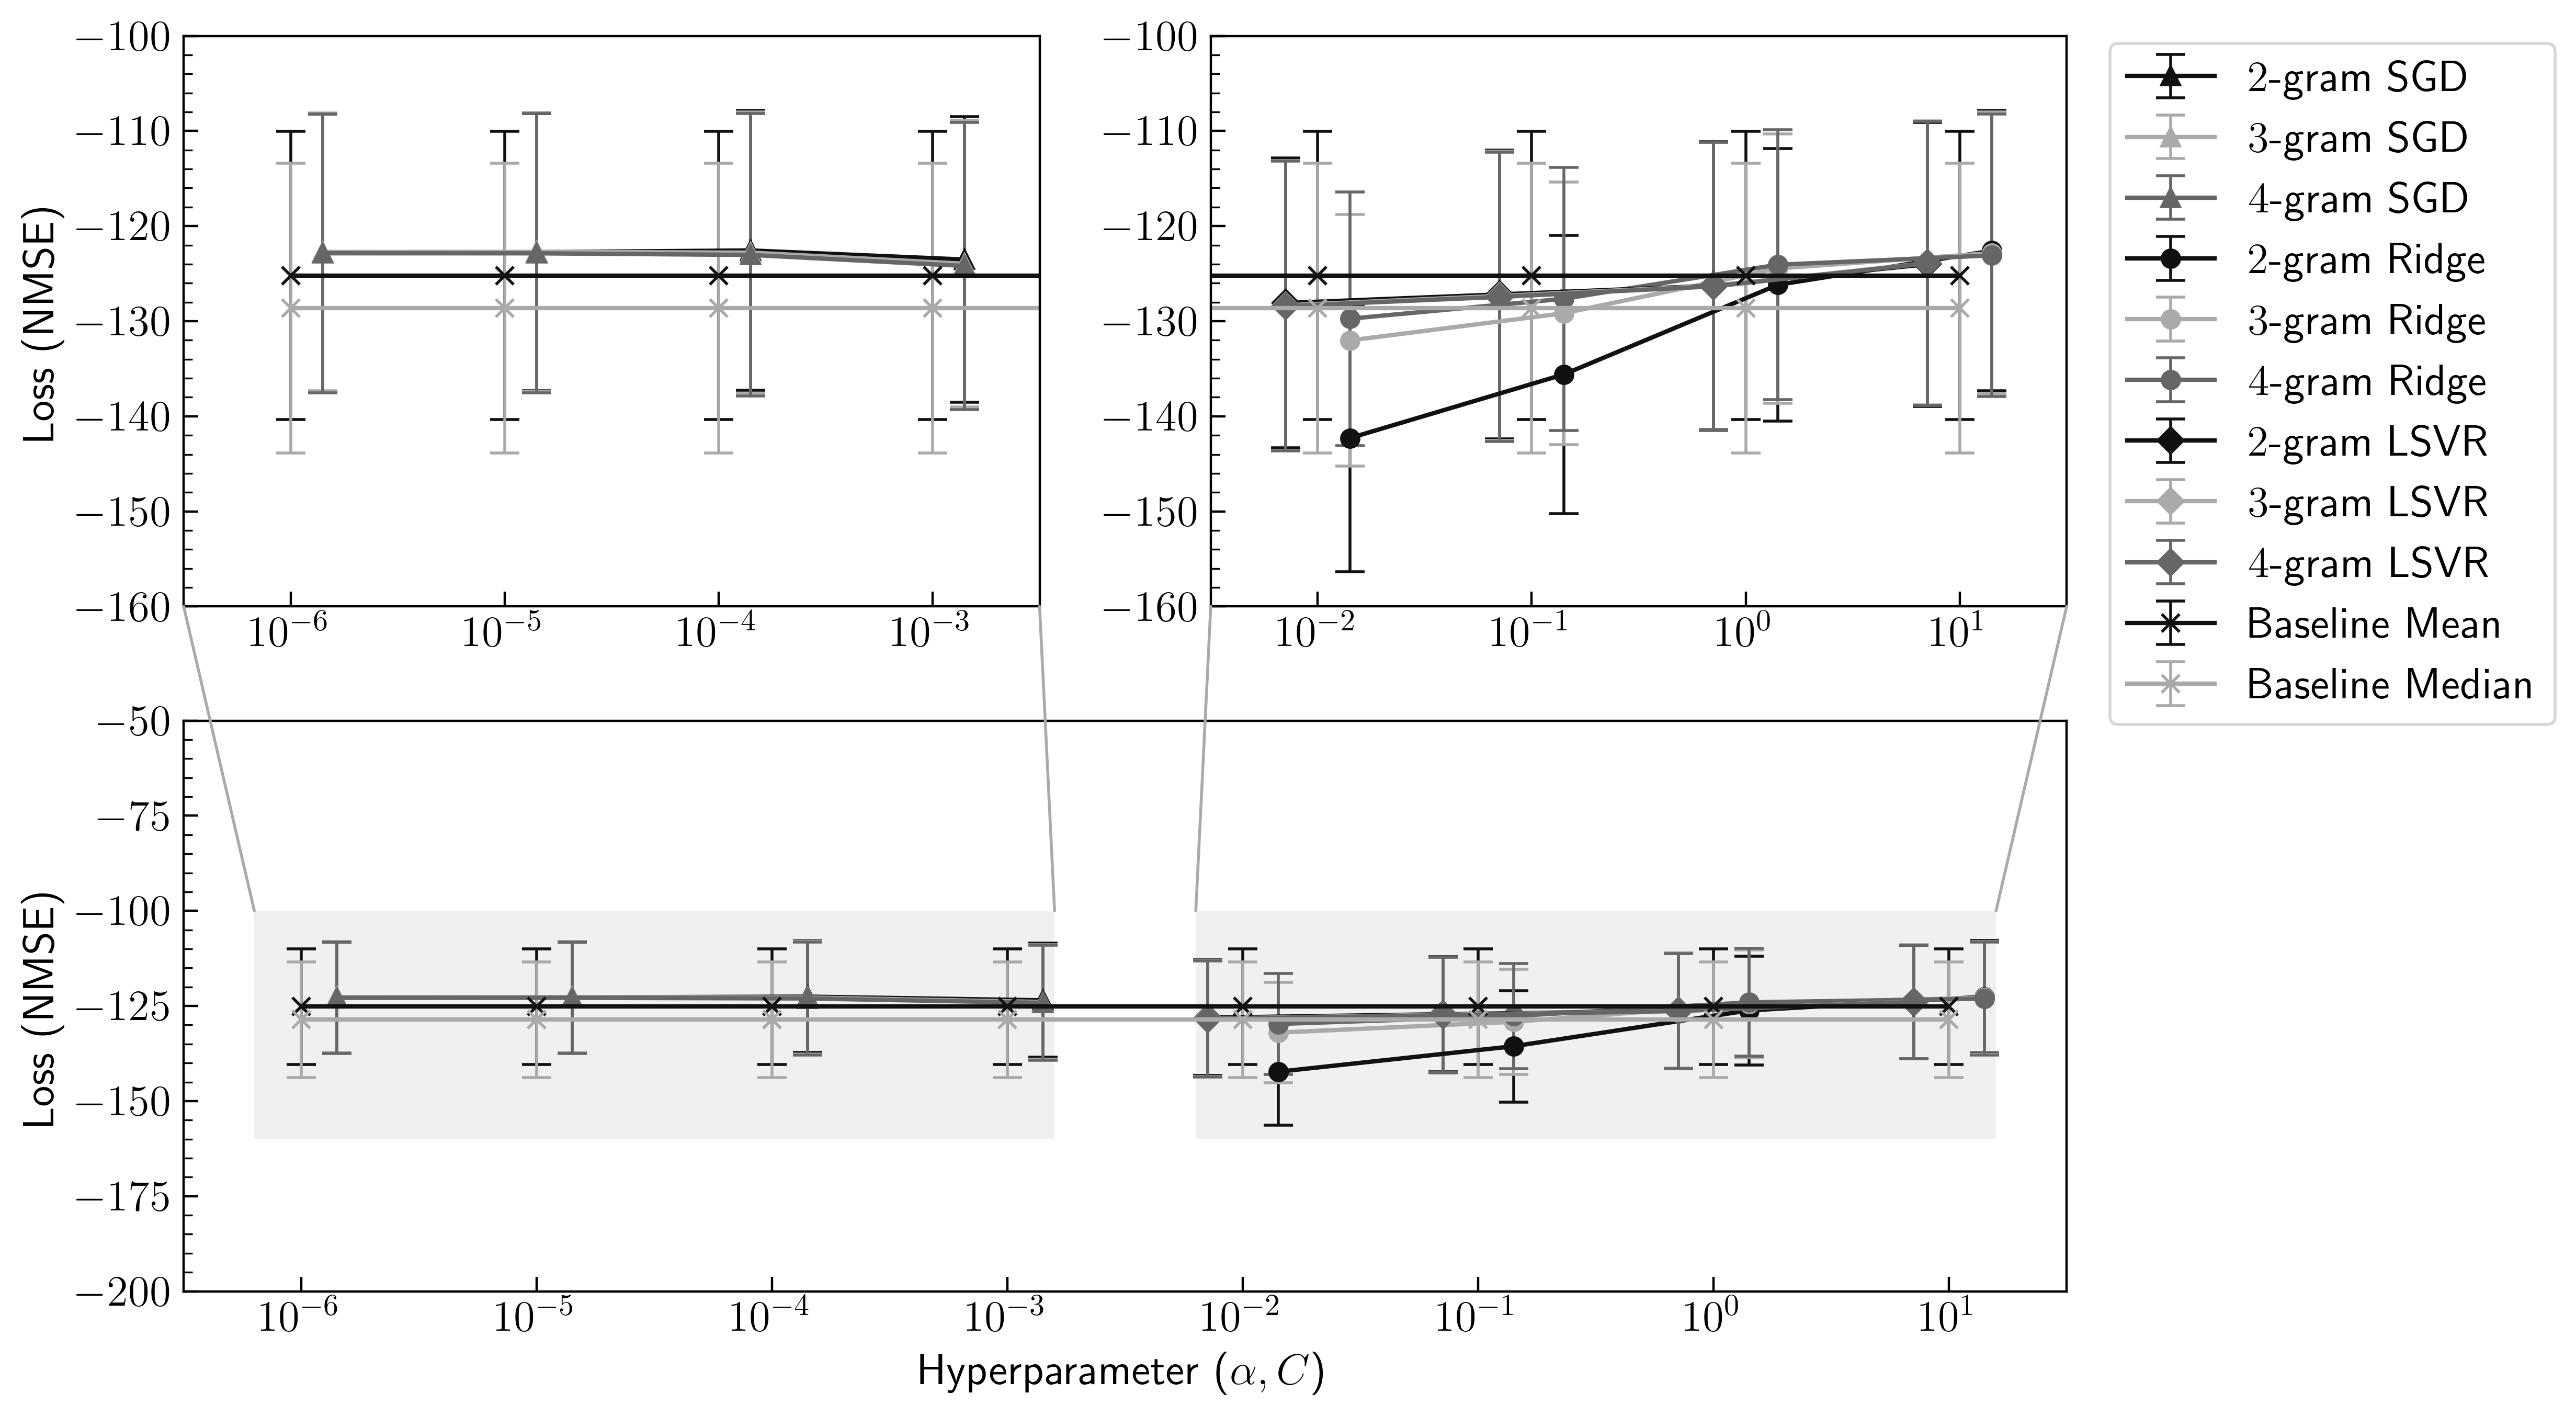
\includegraphics[scale=0.55]{figures/05_impl/01_rfp/02_votes/plot_hyperparams_base.png}
    \caption{Other model hyperparameter tuning results for review votes.}
    \label{fig:DI_RF_Votes_BaseHP}
\end{figure}

The standard deviations of the NMSE losses for each model, despite being quite large, are almost identical and, as such, do not play an important role in determining the optimal choices of hyperparameters.

For the SGD regressor, it would appear that a parameter value of $\alpha=10^{-4}$ with an $n$-gram range of $(1, 2)$ is the best choice; although, no combination of parameters appeared to perform particularly well. For the ridge regressor, the optimal choice is slightly more obvious: a parameter value of $\alpha=10$ with an $n$-gram range of $(1, 2)$ produced the best results. For the LSVR, a parameter value of $\alpha=10$ also produces the best results. An $n$-gram range of $(1, 3)$ produced slightly better results than the other ranges, although this is not clear from the plots alone.

\paragraph{Training Procedure}

Each of the optimal regressors was trained and tested on the 6 imbalanced dataset samples. The test results will be discussed in section \ref{sec:Res_RF_Votes}.

\subsection{Playtime} \label{sec:DI_RF_PT}

The process of training the machine learning models to predict the amount of time that reviewers spent playing the games they reviewed was almost identical to the process used to predict the number of helpfulness votes reviews received.

The data splitting, preprocessing\footnote{A robust scaler was also applied to the playtime values due to a similar presence of outliers.} and training procedure steps involved in the prediction of review playtime, regardless of the model being trained, are identical to the steps given in section \ref{sec:DI_RF_Votes} concerning the prediction of review votes. As such, they have been excluded.

\subsubsection{BERT}

\paragraph{Hyperparameter Tuning}

Optimal training parameters were, again, selected based on the results gathered for the \texttt{eng\_any\_any} sample. Identical combinations of batch size and training epochs were tested and can be seen, once again, in Table \ref{tab:DI_RF_PT_BERTHP}.

\begin{table}[ht]
    \centering
    \begin{tabular}{l l}
        \toprule
        \textbf{Hyperparameter} & \textbf{Values}\\\midrule
        Batch size & $16, 32, 64$\\
        Epochs & $2, 3, 4$\\
        \bottomrule\\
    \end{tabular}
    \caption{BERT hyperparameters for review playtime.}
    \label{tab:DI_RF_PT_BERTHP}
\end{table}

The NMSE loss for both the training and validation sets can be seen in Figure \ref{fig:DI_RF_PT_BERTHP}.

\begin{figure}[ht]
    \centering
    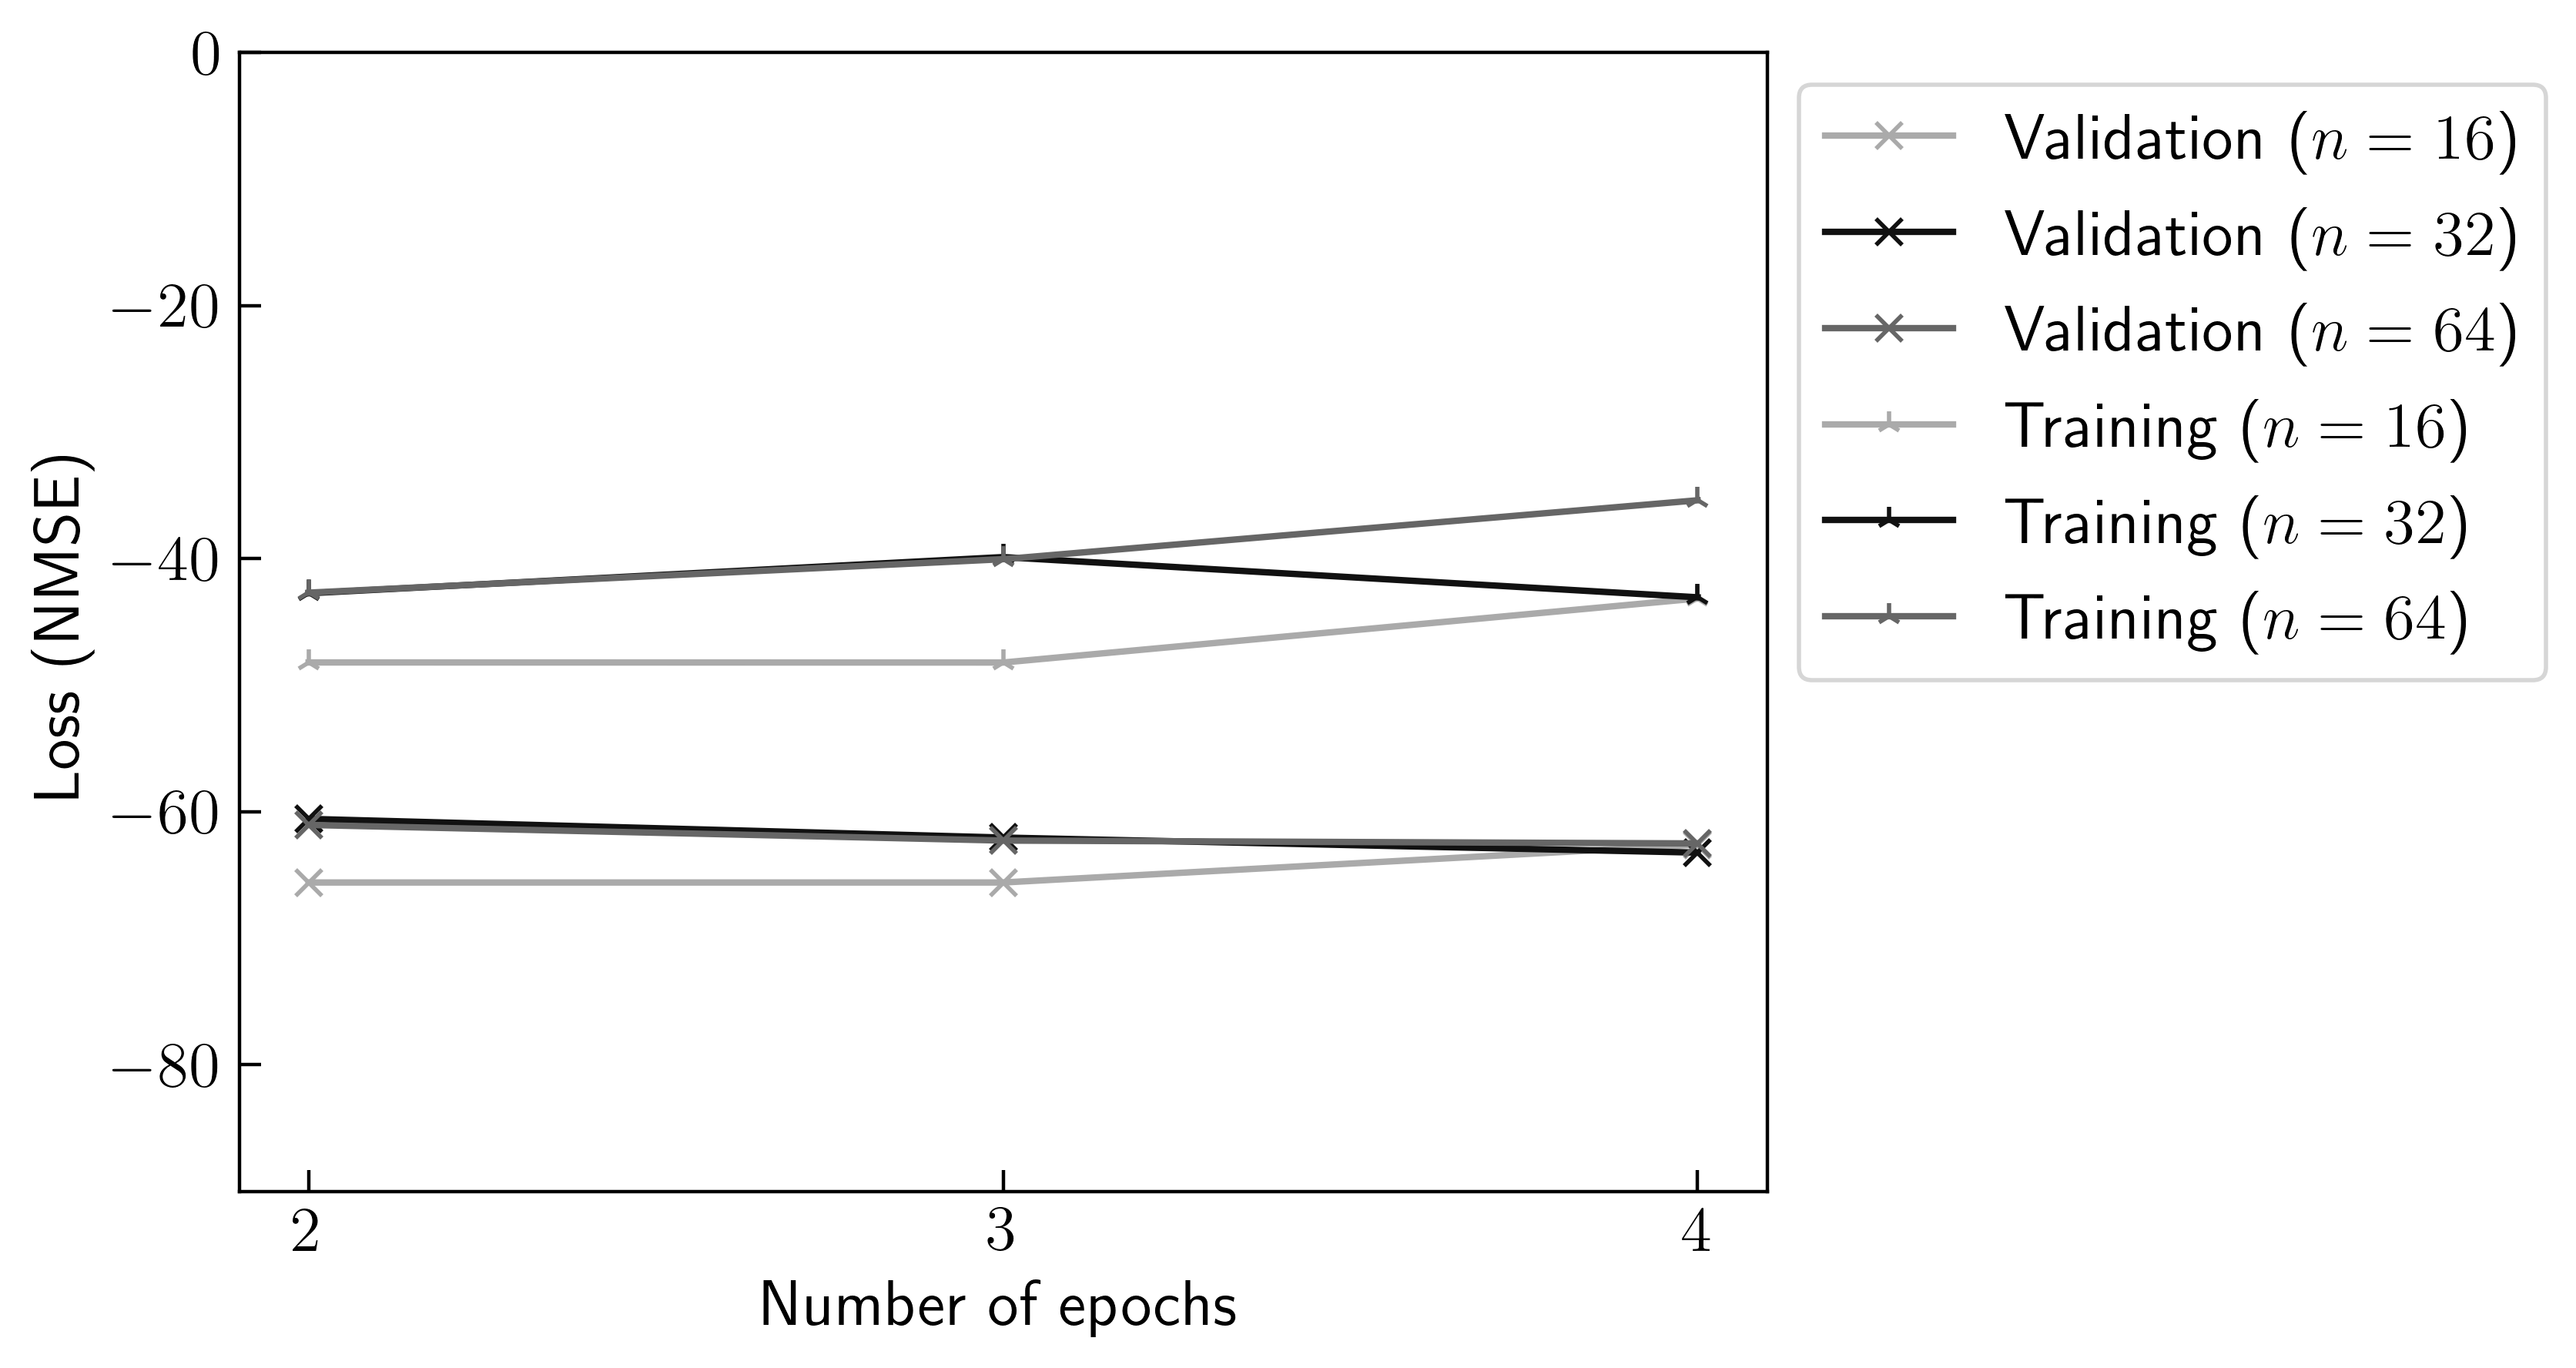
\includegraphics[scale=0.7]{figures/05_impl/01_rfp/03_pt/plot_hyperparams_bert.png}
    \caption{BERT hyperparameter tuning results for review playtime ($n$ is batch size).}
    \label{fig:DI_RF_PT_BERTHP}
\end{figure}

It is quite clear from these results that the optimal choice hyperparameters are batch sizes of 32 or 64 in combination with 2 training epochs, with a batch size of 32 having a slightly better performance\footnote{Due to an initial misreading of the results, a batch size of 64 was chosen when training and testing BERT on the other dataset samples; however, since the NMSE losses for the batch size choices of 32 and 64 were almost identical, this misreading is unlikely to have a significant effect on the overall results.}.

\subsubsection{Other Models}

\paragraph{Hyperparameter Tuning}

The models, hyperparameters and parameter values that were used in the prediction of review votes were also used in the prediction of review playtime. These values can be seen in Table \ref{tab:DI_RF_PT_BaseHP}.

\begin{table}[ht]
    \centering
    \begin{tabular}{l l l}
        \toprule
        \textbf{Model} & \textbf{Hyperparameter} & \textbf{Values}\\\midrule
        All & $n$-gram range & $(1, 2), (1, 3), (1, 4)$\\
        Ridge & $\alpha$ & $0.01, 0.1, 1, 10$\\
        SGD & $\alpha$ & $10^{-3}, 10^{-4}, 10^{-5}, 10^{-6}$\\
        LSVR & $C$ & $0.01, 0.1, 1, 10$\\
        \bottomrule\\
    \end{tabular}
    \caption{Other model hyperparameters for review playtime.}
    \label{tab:DI_RF_PT_BaseHP}
\end{table}

The same two baseline regressors, one that predicted the mean playtime and one that predicted the median playtime, were used for comparison.

The mean cross-validation NMSE losses, along with the standard deviations, can be seen in Figure \ref{fig:DI_RF_PT_BaseHP}. Certain results were, again, offset slightly on the x-axis in order to improve the clarity of the plots.

\begin{figure}[ht]
    \hspace*{-0.3in}
    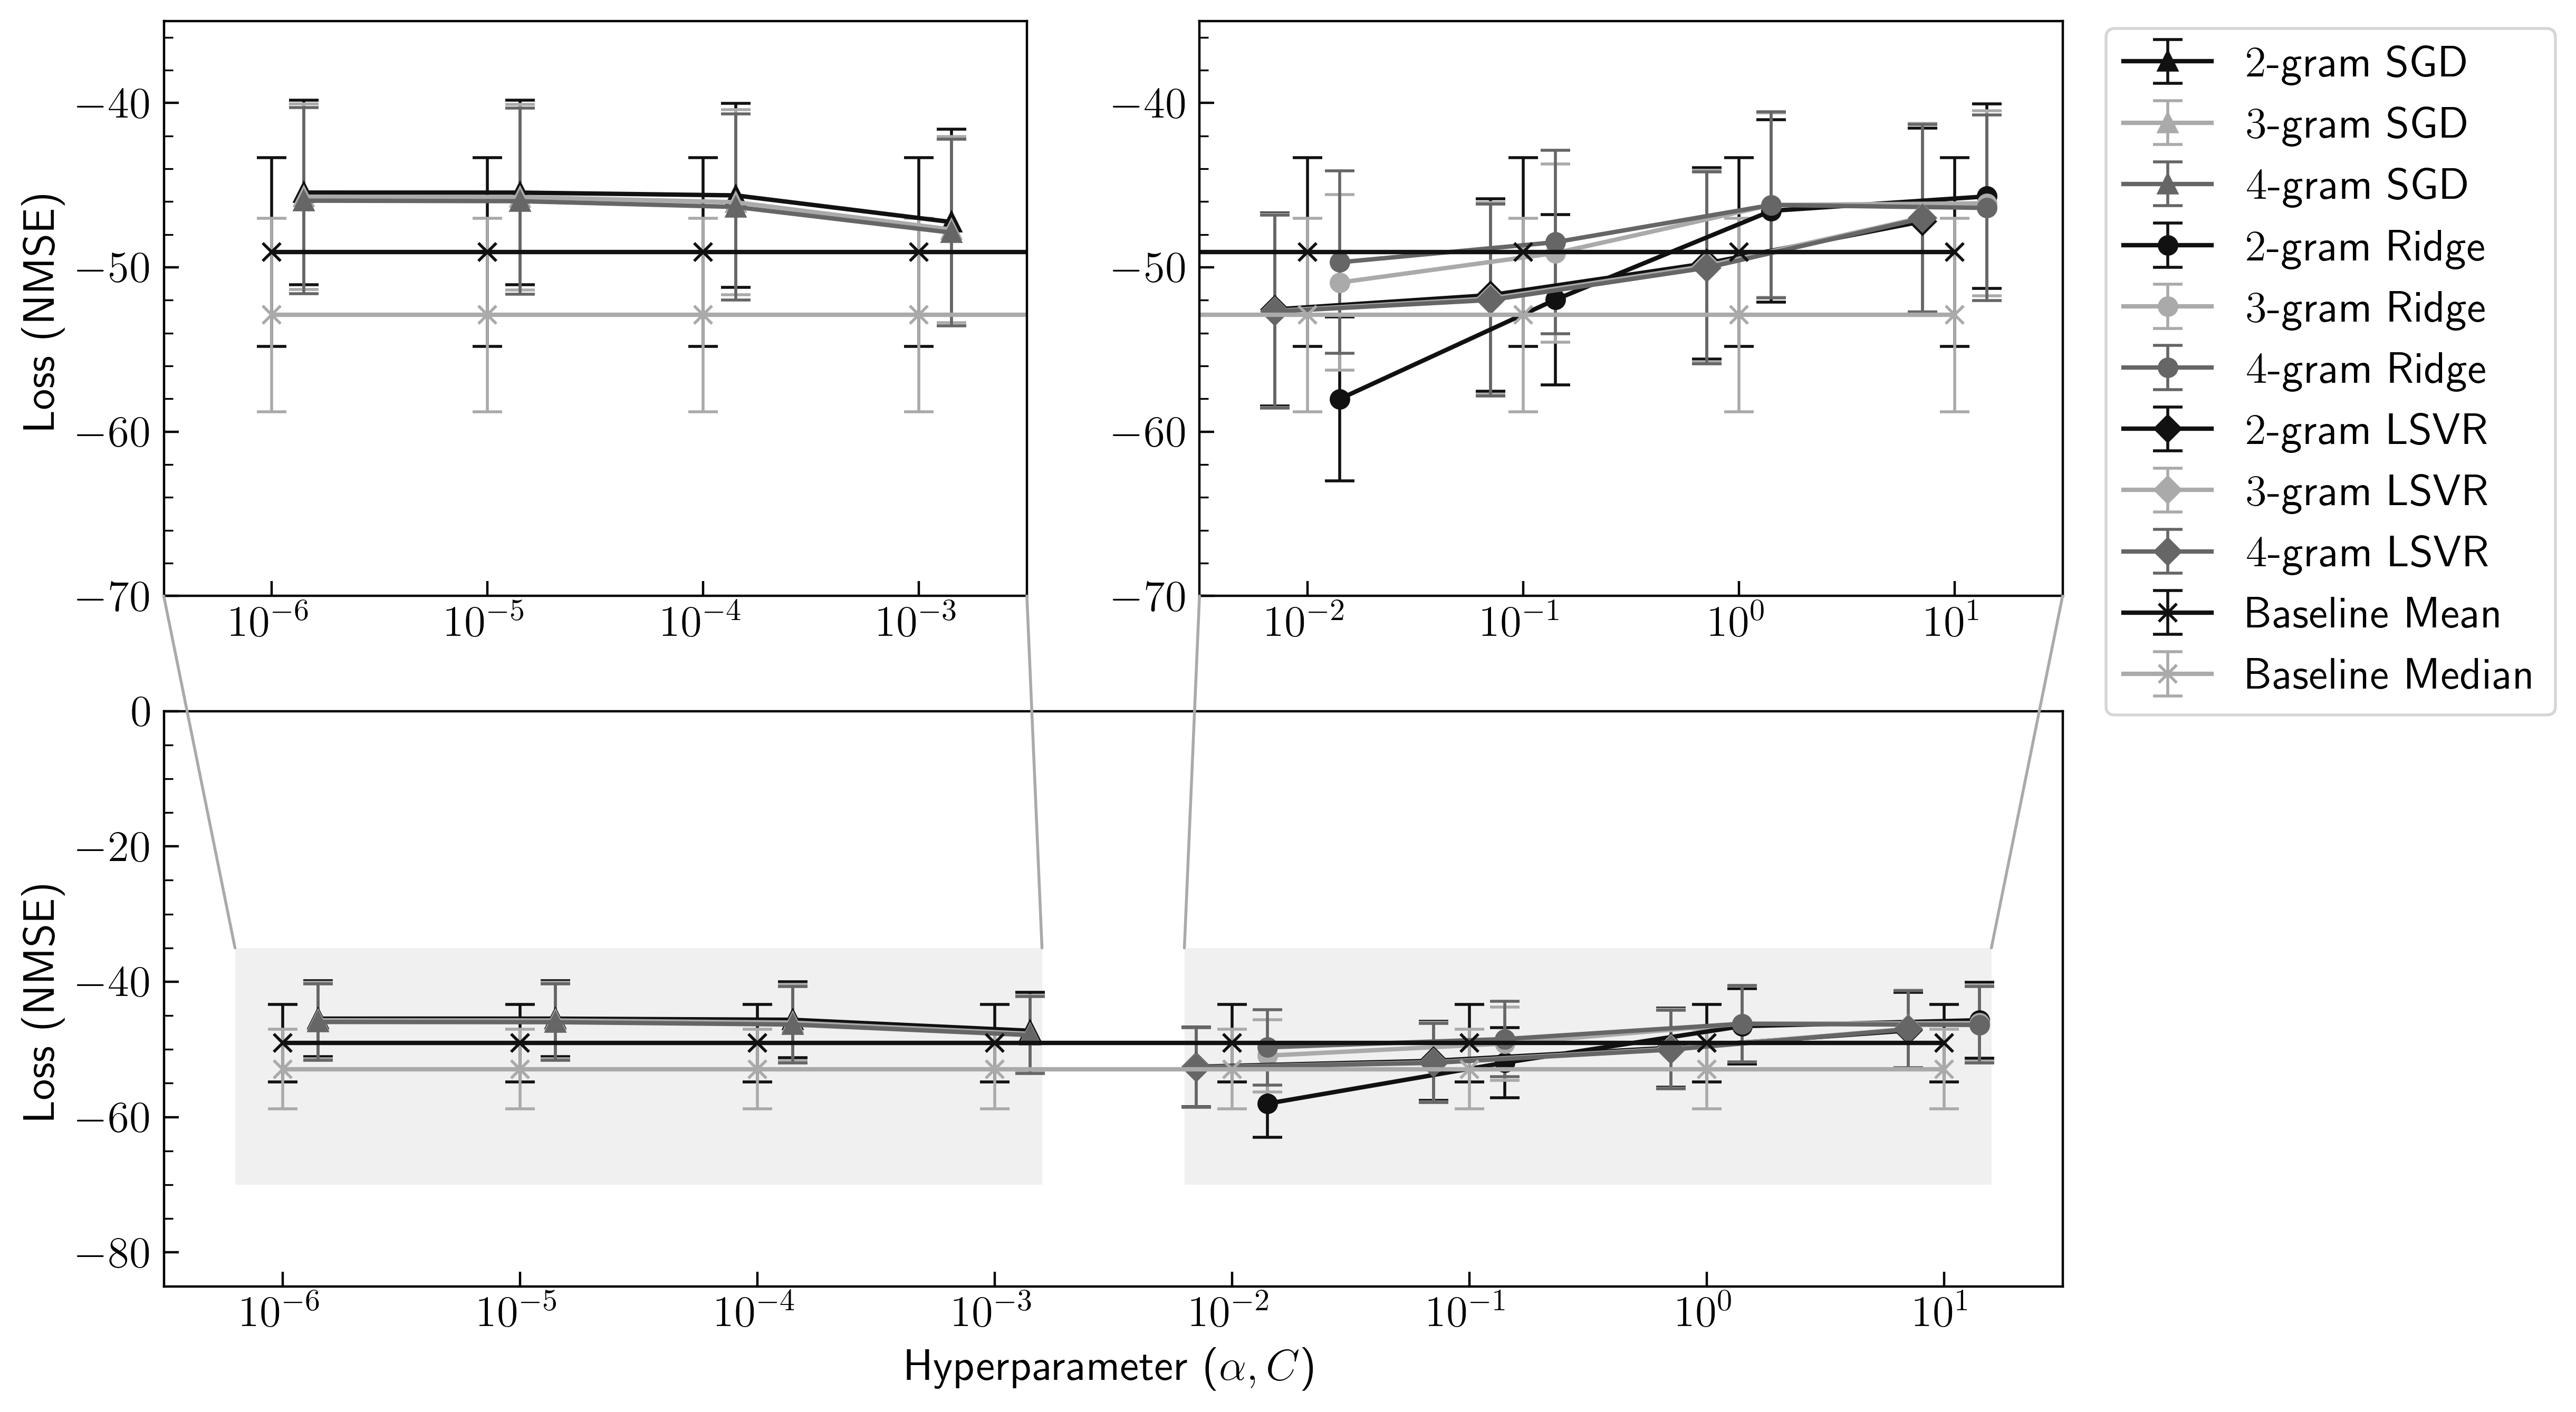
\includegraphics[scale=0.55]{figures/05_impl/01_rfp/03_pt/plot_hyperparams_base.png}
    \caption{Other model hyperparameter tuning results for review playtime.}
    \label{fig:DI_RF_PT_BaseHP}
\end{figure}

The standard deviations of the NMSE losses for each model do not play an important role in the selection of hyperparameters for the same reasons listed in \ref{sec:DI_RF_Votes}.

For the SGD regressor, the $n$-gram range of $(1, 2)$ clearly produces the best results, with the parameter value of $\alpha=10^{-5}$ performing slightly better than the other options. For the ridge regressor, the optimal choices of an $n$-gram range of $(1, 2)$ and a parameter value of $\alpha=10$ are quite clear. For the LSVR, a value of $C=10$ is clearly the optimal choice. Although it isn't clear from the plot, an $n$-gram range of $(1, 3)$ produces the best results when $C=10$.

\section{Representative Users} \label{sec:DI_RU}

In this section, the process of selecting and training optimal machine learning models with the goal of identifying users whose written reviews best represent the views of the total population will be discussed. The machine learning models that will be tested are the previously discussed DistilBERT models; MNB and CNB classifiers; a linear SVM classifier, both with SGD and without; and multiple baseline classifiers.

\subsection{Methodology}

The methodology underpinning this approach can be described as follows:

\begin{enumerate}
    \item Select the reviews of users who've written at least $N$ reviews.
    \item Calculate the average rating, across the entire dataset, for each of the games being reviewed.
    \item Convert these ratings into classes that correspond to Steam's own rating classification scheme.
    \item Train models to predict the rating class of a game being reviewed using only the review text.
    \item Test this model on a per-user basis and determine the users whose reviews are predicted most accurately.
    \item These users could be considered `representative' of the reviewer population.
\end{enumerate}

Much of the steps involved in this approach are essentially extensions to the work done to predict a review's polarity in section \ref{sec:DI_RF_Pol}. The goal, in this case, is to train a multiclass classifier to predict the average polarity of a game based on all of its reviews, rather than to predict the binary class of an individual review.

A potential drawback to this approach is that, given a game with a positive rating of 70\%, we would expect 30\% of the review texts for that game, ie the negative ones, to portray a noticeably negative sentiment. This could be problematic since, in this example, 30\% of the training data could be considered bad or of poor quality because the overall rating ought to be fairly positive. A key assumption is made in an attempt to overcome this drawback. This assumption is as follows: since a significant majority of the review data being processed for each game does actually align with its overall rating, the predictive model ought to be able to, on average, favour the good data and ignore the bad, ie noisy, data since there always exists much more good data.

Another assumption made by this approach is that there are features within the review texts which occur more frequently for games of different average ratings. For example, we might expect extremely positive words like `amazing' or `fantastic' to occur more in reviews for games with a positive rating of 95\% than in reviews for games with a positive rating of 70\%. The hope is that the trained model will be able to discern these particular features from the otherwise noisy data.

\subsection{Dataset Sampling and Preparation}

Numerous samples of the dataset, each containing exactly 160 thousand reviews, were prepared and used to train the predictive models.

First, reviews consisting of less than one word and reviews for `early access' games were excluded from the dataset. Reviews for games with fewer than 50 total reviews were also excluded. Finally, out of those reviews remaining, the reviews of users who had written fewer than 10 written reviews were excluded.

For those reviews that remained, the average rating for each game was calculated and mapped to one of either 3 or 6 classes. These classes were chosen and named based roughly on the chart shown in Figure \ref{fig:SteamStore_Ratings}. The details of each of these sets of classes are given in Table \ref{tab:DI_PU_Classes6} and Table \ref{tab:DI_PU_Classes3}, respectively.

\begin{table}[ht]
    \centering
    \begin{tabular}{l l l}
        \toprule
        \textbf{Name} & \textbf{Acronym} & \textbf{Rating Range}\\\midrule
        Very Positive & VP & $[0.95, 1.0]$\\
        Positive & P & $[0.8, 0.95)$\\
        Mostly Positive & MP & $[0.7, 0.8)$\\
        Mixed & M & $[0.4, 0.7)$\\
        Mostly Negative & MN & $[0.2, 0.4)$\\
        Negative & N & $[0.0, 0.2)$\\
        \bottomrule\\
    \end{tabular}
    \caption{Game rating classes used in 6-class approach.}
    \label{tab:DI_PU_Classes6}
\end{table}

\begin{table}[ht]
    \centering
    \begin{tabular}{l l l}
        \toprule
        \textbf{Name} & \textbf{Acronym} & \textbf{Rating Range}\\\midrule
        Positive & P & $[0.7, 1.0]$\\
        Mixed & M & $[0.4, 0.7)$\\
        Negative & N & $[0.0, 0.4)$\\
        \bottomrule\\
    \end{tabular}
    \caption{Game rating classes used in 3-class approach.}
    \label{tab:DI_PU_Classes3}
\end{table}

Since the goal of this task is to determine representative users, it is important that, for any particular user with reviews in a dataset sample, all of the valid reviews they've written are included and none of these reviews are split across different sample splits, eg the training and test splits. Because of this requirement, the training, validation and test splits were prepared in advance, rather than at runtime. The sample splitting was carried out so that the reviews of 80\% of users were in the training set, the reviews of 10\% of users were in the validation set and the reviews of the remaining 10\% of users were in the test set.

Separate samples were prepared for reviews written in English and reviews written in any language (including English). The names and characteristics of all of the prepared data samples are given in Table \ref{tab:DI_PU_Samples}.

\begin{table}[ht]
    \centering
    \begin{tabular}{l|l l l}
        \toprule
        \textbf{Sample Name} & \textbf{Language} & \textbf{Classes} & \textbf{Size}\\\midrule
        \texttt{eng\_6} & English & 6 & 160k\\
        \texttt{eng\_3} & English & 3 & 160k\\
        \texttt{any\_6} & Multilingual & 6 & 160k\\
        \texttt{any\_3} & Multilingual & 3 & 160k\\
        \bottomrule
    \end{tabular}
    \caption{Dataset samples and their characteristics for determining representative users.}
    \label{tab:DI_PU_Samples}
\end{table}

\subsection{BERT}

\subsubsection{Preprocessing}

As was the case when predicting the polarity of reviews, very little preprocessing was needed before passing the data into the BERT model for training. The data, which had already been split into training, validation and test sets, were converted to tensors and used to fit the BERT classifier.

\subsubsection{Hyperparameter Tuning}

Optimal training parameters were selected for all of the models using the results gathered by training models on the \texttt{eng\_6} sample. The same BERT hyperparameters that were varied when predicting the review features were also varied in this approach. The considered values can be seen in Table \ref{tab:DI_PU_BERTHP}.

\begin{table}[ht]
    \centering
    \begin{tabular}{l l}
        \toprule
        \textbf{Hyperparameter} & \textbf{Values}\\\midrule
        Batch size & $16, 32, 64$\\
        Epochs & $2, 3, 4$\\
        \bottomrule\\
    \end{tabular}
    \caption{BERT hyperparameters for representative users.}
    \label{tab:DI_PU_BERTHP}
\end{table}

The training and validation accuracies of the trained models for each combination of hyperparameters can be seen in Figure \ref{fig:DI_PU_BERTHP}.

\begin{figure}[ht]
    \centering
    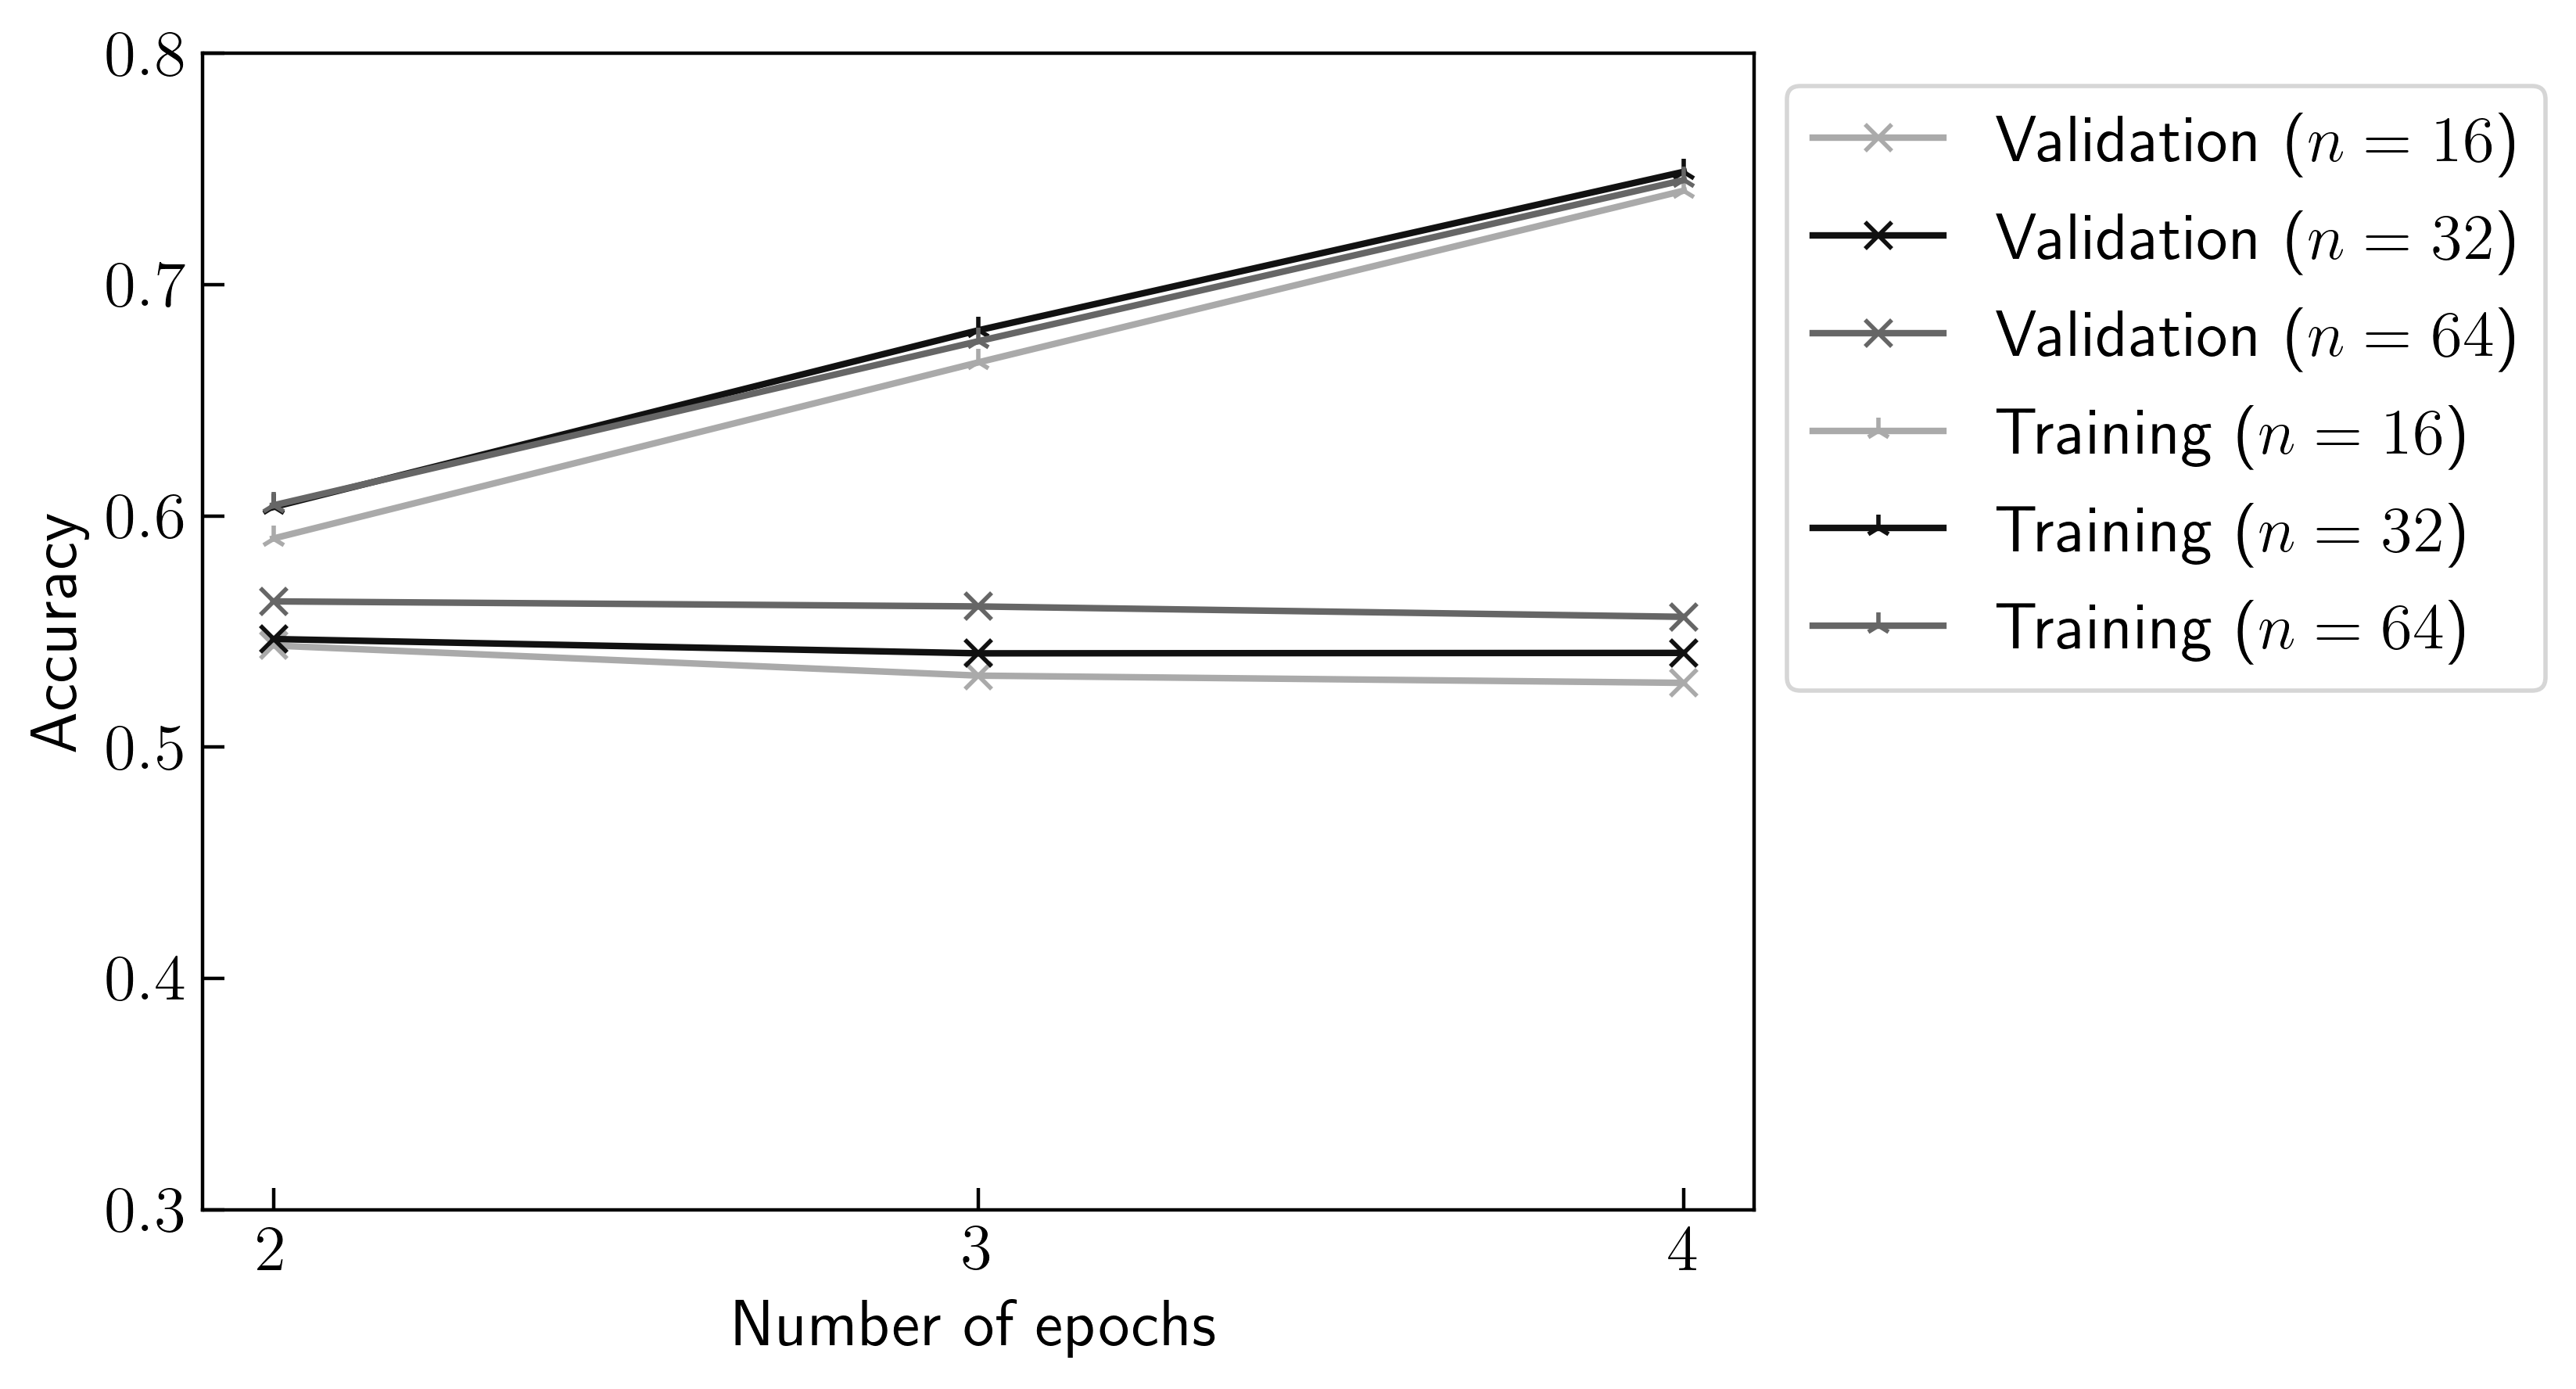
\includegraphics[scale=0.7]{figures/05_impl/02_pu/plot_hyperparams_bert.png}
    \caption{BERT hyperparameter tuning results for representative users ($n$ is batch size).}
    \label{fig:DI_PU_BERTHP}
\end{figure}

Based on these results it would appear that 2 training epochs with a batch size of 64 are the optimal combination of parameters. Interestingly, the validation and training accuracies for this combination are nearly identical, indicating that the model is neither underfitting nor overfitting the training data.

\subsubsection{Training and Testing Procedure}

BERT models were trained and validated for all 4 dataset samples using the aforementioned combination of hyperparameters and the appropriate choice of pretrained DistilBERT model, which depended on the language of the samples' reviews. Their performance was then tested using the relevant test set. The overall results of these tests, as well as the user-specific results, will be discussed in section \ref{sec:Res_RU}.

\subsection{Other Models}

\subsubsection{Preprocessing}

The same preprocessing steps taken when predicting review polarities for non-BERT models in section \ref{sec:DI_RF_Pol} were also taken here. One important difference was that the previously prepared training and validation splits were merged into a single training set containing the reviews of 90\% of users.

\subsubsection{Hyperparameter Tuning}

Optimal model parameters were again selected based on the results taken from the \texttt{eng\_6} sample.

The models, hyperparameters and values that were varied were identical to those used in section \ref{sec:DI_RF_Pol}. These values can be seen in Table \ref{tab:DI_PU_BaseHP}.

\begin{table}[ht]
    \centering
    \begin{tabular}{l l l}
        \toprule
        \textbf{Model} & \textbf{Hyperparameter} & \textbf{Values}\\\midrule
        All & $n$-gram range & $(1, 2), (1, 3), (1, 4)$\\
        MNB & $\alpha$ & $0.01, 0.1, 1, 10$\\
        CNB & $\alpha$ & $0.01, 0.1, 1, 10$\\
        SGD & $\alpha$ & $10^{-4}, 10^{-5}, 10^{-6}$\\
        LSVC & $C$ & $0.01, 0.1, 1, 10$\\
        \bottomrule\\
    \end{tabular}
    \caption{Other model hyperparameters for representative users.}
    \label{tab:DI_PU_BaseHP}
\end{table}

Two baseline classifiers were also used for comparison: one which predicted the most frequent class and one which predicted a random class based on the overall distribution of the classes in the dataset. The mean cross-validation accuracies can be seen in Figure \ref{fig:DI_PU_BaseHP}. The standard deviations, as was the case when predicting review polarities, were found to be insignificantly small and, as such, have not been included.

\begin{figure}[ht]
    \hspace*{-0.3in}
    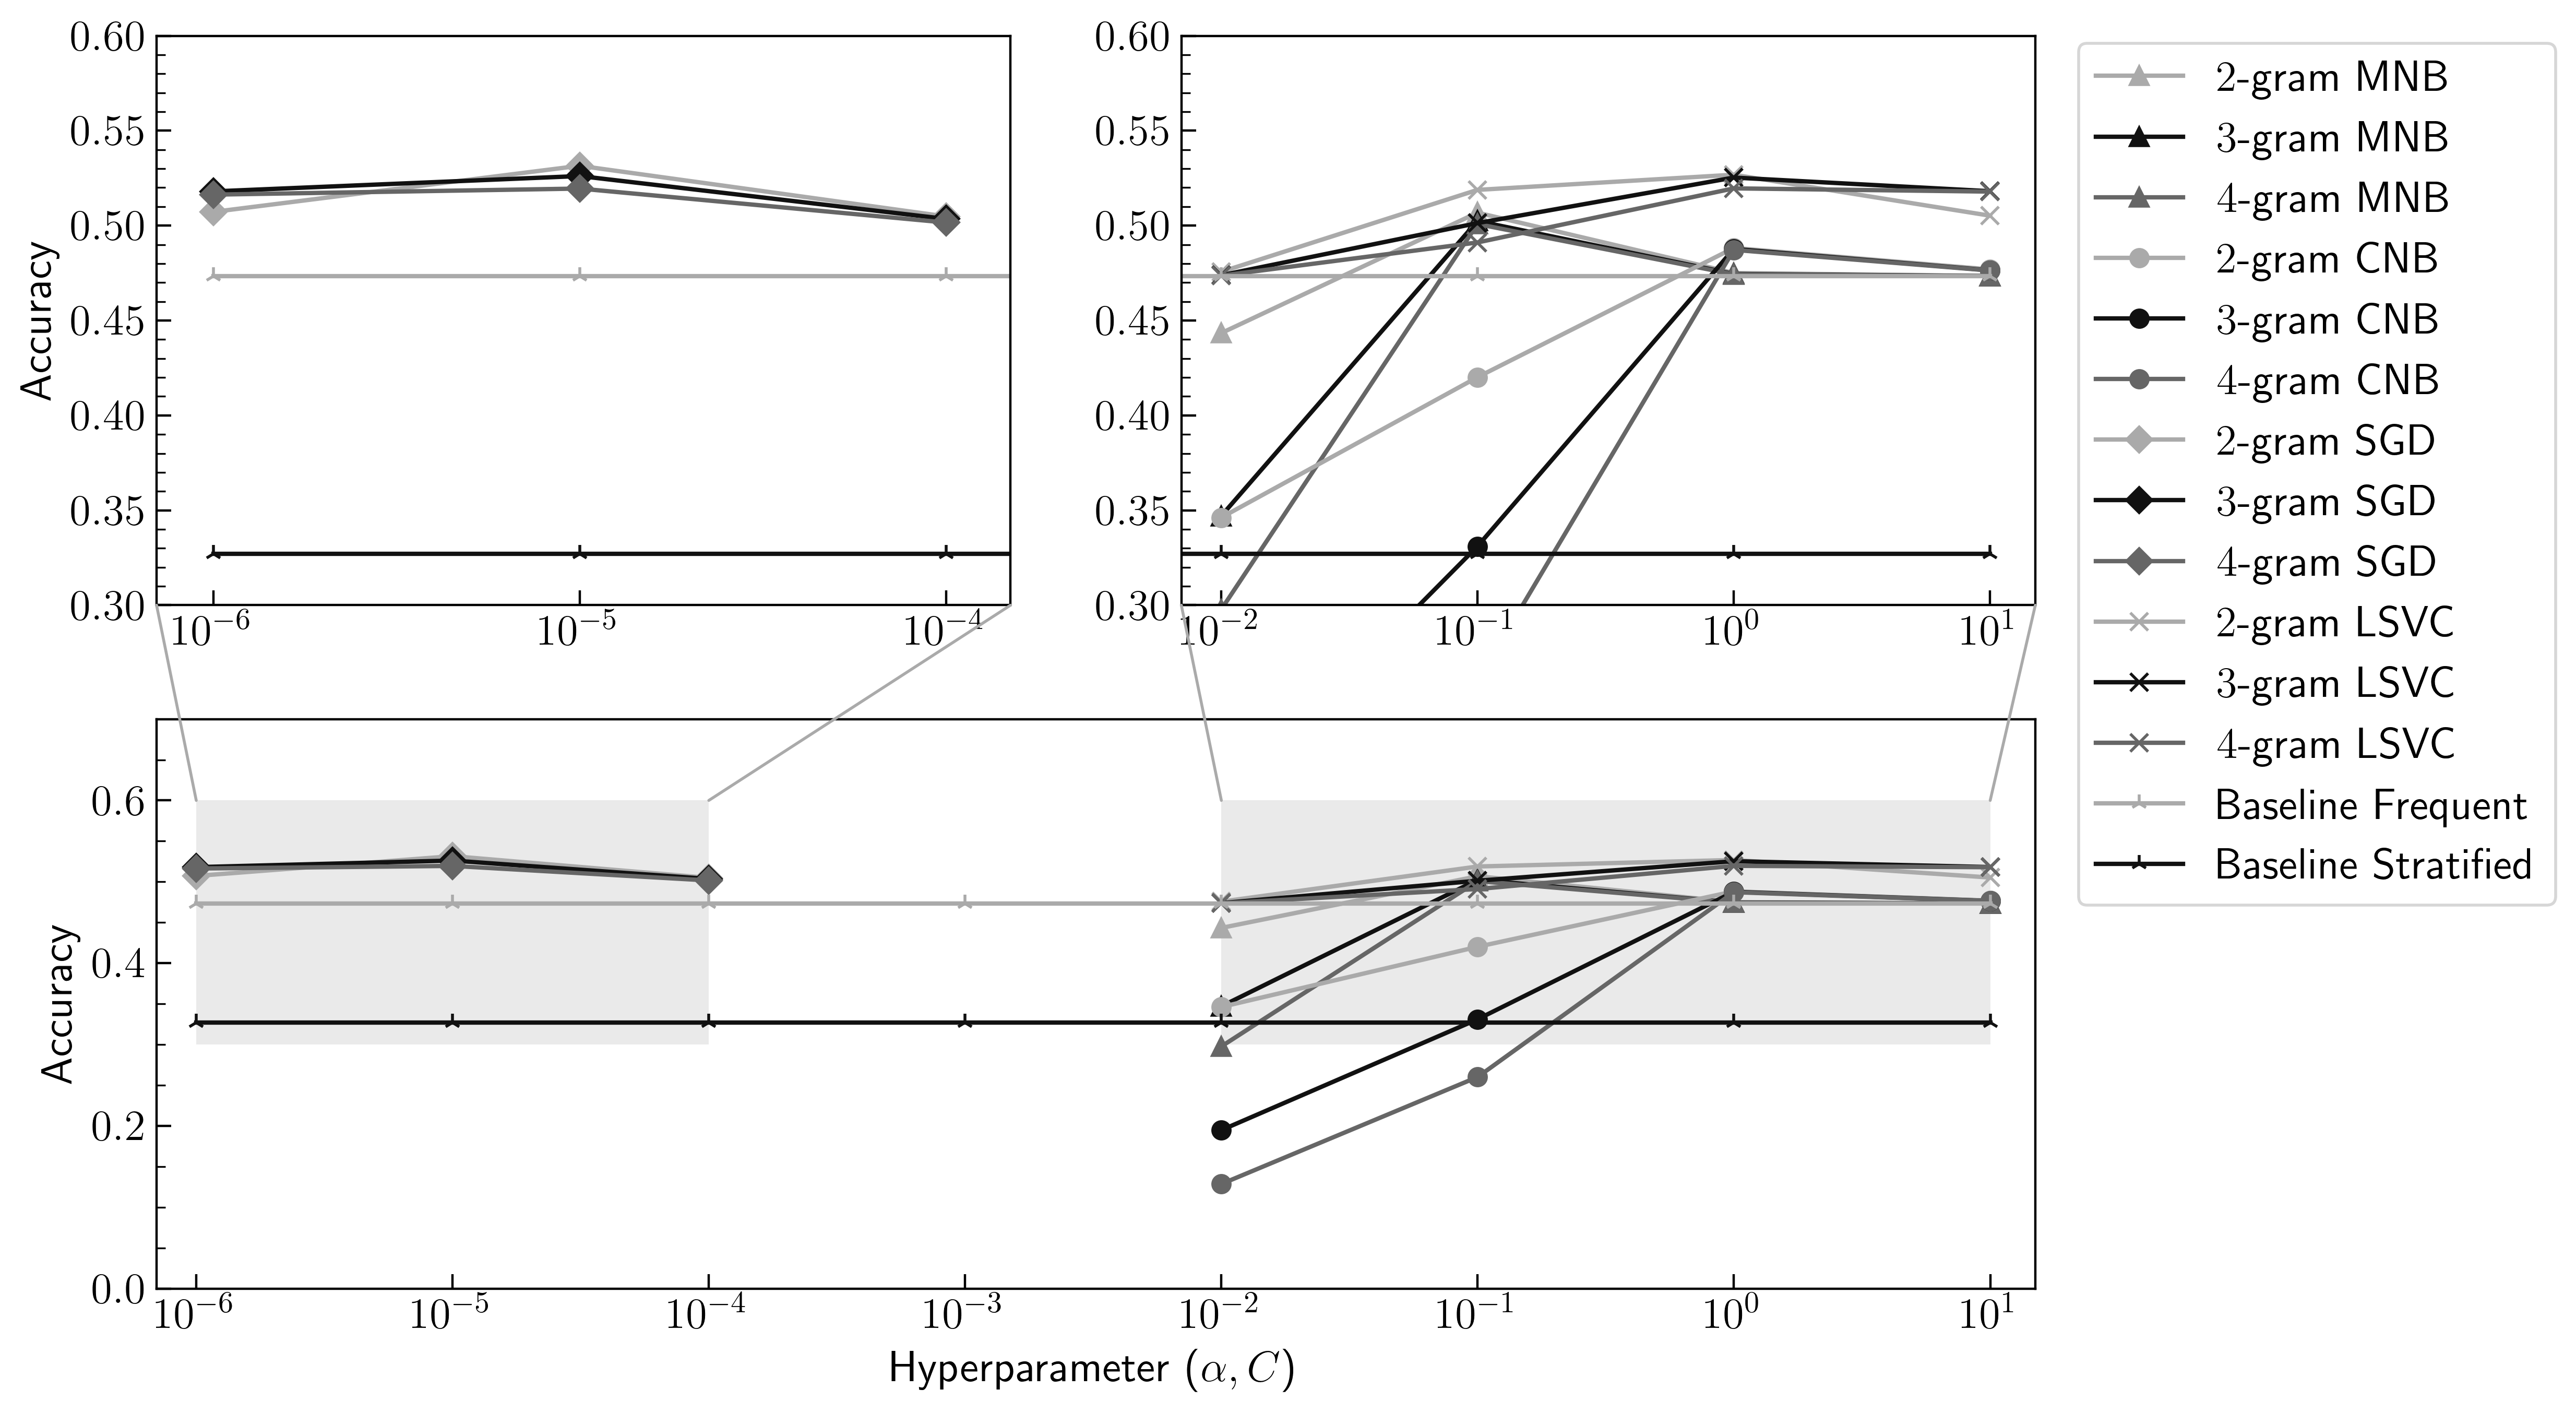
\includegraphics[scale=0.55]{figures/05_impl/02_pu/plot_hyperparams_base.png}
    \caption{Other model hyperparameter tuning results for representative users.}
    \label{fig:DI_PU_BaseHP}
\end{figure}

For the SGD classifier, it is quite clear that the optimal choice of hyperparameters is an $n$-gram range of $(1, 2)$ and a parameter value of $\alpha=10^{-5}$. For both NB classifiers, an $n$-gram range of $(1, 2)$ produced the best results. A parameter value of $\alpha=0.1$ produced the best results for the MNB classifier, while a value of $\alpha=1$ produced the best results for the CNB classifier. Finally, for the LSVC, the combination of hyperparameters that performed the best was an $n$-gram range of $(1, 2)$ with a parameter value of $C=1$. Interestingly, regardless of the classifier in question, an $n$-gram range $(1, 2)$ always produced better results than the other ranges.

\subsubsection{Training and Testing Procedure}

Models were trained and tested for all of the dataset samples using the optimal choices of hyperparameters. As was the case with the BERT model, the performance of the models was evaluated with regard to the entire test set as well as on a per-user basis. These results will be discussed in section \ref{sec:Res_RU}.

\chapter{Results} \label{sec:Res}

\section{Review Feature Prediction} \label{sec:Res_RF}

Text.

\subsection{Polarity} \label{sec:Res_RF_Pol}

Text.

\subsection{Votes} \label{sec:Res_RF_Votes}

Text.

\subsection{Playtime} \label{sec:Res_RF_PT}

Text.

\section{Representative Users} \label{sec:Res_RU}

Text.

\chapter{Conclusion} \label{sec:Conc}

In this report, state-of-the-art text representation models were trained to predict a selection of Steam review features using only the written text of the review. In the case of review polarities, the results showed that the trained models could predict this feature with a very high degree of accuracy. In additional experiments, certain factors, such as the length of the reviews and the languages they were written in, were controlled for, and the results were evaluated and compared. In each case, the trained models produced consistently strong results.

The results of the models trained to predict the number of votes that reviews received indicated that the employed approach did not produce predictions that were accurate. The models trained to predict how long each reviewer had spent playing the game they were reviewing did appear to be capable of making predictions that were partially accurate, at least when compared to a suitable baseline.

Influenced by the success of the models trained to predict review polarity, the same state-of-the-art text representation techniques were used to predict the average ratings of the games being reviewed using each individual sample of review text. Certain trained models, despite the abundance of bad or noisy data, were able to make predictions that were more accurate than their respective baselines to a significant enough degree that further investigation appeared to be warranted. These trained models were then used to determine which users could be considered the most representative of the total population based on their individual, average accuracies, relative to a baseline predictor. The apparent feasibility of this approach suggests that particularly representative users could be determined using only the raw review text, without any manual selection, filtering or preparation processes being applied to the training data.

The research objectives outlined in this report's introduction were carried out successfully, with intriguing results being provided in every case. The investigation into representative users appears to be the most compelling, for two reasons in particular. Firstly, there are many refinements and improvements that could be made to both the methodology underpinning the approach and the implementation of the technical solution. Secondly, the determination of representative users might potentially have real-world, commercial applications. For example, the approach could be used by media recommendation systems to estimate the quality of newly released products by initially recommending the product to particularly representative users and accurately extrapolating, based on their responses, how popular the product will be among the overall user base. This estimation of quality and potential popularity could then be incorporated into the recommendation system's behaviour to help it decide how frequently or aggressively it should suggest the product in question to average users.
 
\section{Future Work} \label{sec:Conc_FW}

Many of the alternatives or improvements to the approach taken when predicting review polarity have been discussed already, mainly involving the training of the BERT models on larger samples of data. Language-specific samples could also be created for some of the more prevalent languages in the dataset, such as Russian or Chinese, and these could be used to fine-tune BERT models which have already been trained for these particular languages. Additional features could be controlled for when selecting review texts to sample, such as the number of votes the review received or the playtime of the reviewer. The results from these more restrictive samples could provide insight into the factors which affect how accurately review polarity can be predicted. An interesting, though slightly tangential approach, would be to apply a simplified version of the `representative user' analysis method to this task and determine if there exist users whose reviews are particularly easy to classify, polarity-wise.

Much of the additional work that could be done regarding the prediction of review votes and review playtime has already been discussed. The suggested alternative approaches mainly involved transforming the problem from one of regression into one of classification. This would essentially involve the models predicting percentile-based classes rather than exact values, with regard to either the number of votes reviews received or the amount of playtime reviewers had logged. Data balancing techniques, such as excluding reviews without any votes, were also considered and discussed.

The amount of training data supplied to the models used to identify representative users could be hugely increased. In order to increase the quality of the training data, more restrictive sampling methods could be employed, such as only selecting reviews with a certain number of votes or containing a certain number of words. More balanced data samples could also be created in order to reduce the heavy bias towards games with a rating of `positive'.

One of the benefits of the implementation outlined in this report is that it does not require any manual intervention with regard to the labelling of review classes or the filtering of data; however, an obvious, drawback to this approach is the inclusion of bad data in the training set. A number of fully automated or partially automated processes could be used to reduce the prevalence of poor quality or unrepresentative reviews among the training data.

For example, reviews whose texts are not accurately classified by the polarity prediction models could be excluded. Certain text features, such as the readability or writing level, could be considered when sampling the data, while more complex methods, such as those discussed in sections ? and ?, could also be incorporated into the sampling process. Finally, suitable training data could be manually selected and, although it would be time-consuming, this approach would almost certainly lead to a far more accurate model. In summary, though only a small set of potential improvements to the approach utilised in this report have been listed above, it seems likely that this technique could be refined and developed to be considerably more successful.

The model used to determine representative users could be expanded to consider the communities or `clusters' that each user is a part of, thus allowing the model to determine not only how representative individual users are of the entire population, but also of certain subsets of the population.

The dataset also consists of millions of data points concerning the social relationships between reviewers, ie friendship and group membership. These portions of the dataset, though briefly discussed and examined in section ?, were not actually utilised in the design, implementation or training of any of the models used throughout this report. In future work, these data could be used to, for instance, determine potentially influential users, ie those whose reviews result in their friends or fellow group members being more likely to play the games being reviewed. The knowledge of which users are influential and which users are representative could be combined and used to improve the way in which games are recommended by Steam. For example, after initially recommending a new game to a pool of representative users, the recommendation system could then, if it has estimated that the game is of high quality, recommend it to particularly influential users in order to help spread it a wider audience.


\bibliographystyle{unsrtnat}
\bibliography{bibs/main}

\appendix
\renewcommand{\thechapter}{A\arabic{chapter}}
\chapter{Appendix 1}

Text.

\chapter{Code Repository} \label{sec:A2}

The code carry out the research in this dissertation can be found in the following GitHub repository: \url{https://github.com/conormccauley1999/MCSDissertation}.


\end{document}
